%\documentclass[12pt,a4paper]{article} % A4 paper and 11pt font size
\documentclass[12pt]{thesis}  % default square logo 


\usepackage[utf8x]{inputenc}
\usepackage{braket}
\usepackage{amsmath}
\usepackage{amssymb}
\usepackage{bm}
%\usepackage[utf8]{inputenc}
\usepackage{verbatim}
\usepackage{tikz}
%\usepackage{tikz-feynman}
%\usepackage{pgfornament}
\usepackage{pgfplots}
\usepackage{pgffor}
\usepackage[version-1-compatibility]{siunitx}
\usepackage{fancyhdr}
\usepackage{lipsum}
%\usepackage{gensymb}
\usepackage{framed}
\usepackage{cancel}
\usepackage{slashed}
\usepackage{hyperref}
\usepackage{pdflscape}
\usepackage{graphicx}
\usepackage{caption}
\usepackage{subcaption}
\usepackage{geometry}
\usepackage{yfonts}
\usepackage{calc}
\usepackage{cite}

\usepackage{caption}
\usepackage{subcaption}

% rotated tables (and figures if necessary)
%\usepackage{fullpage}
\usepackage{graphicx}
\usepackage{rotating}



%%%%%%%%%%%%%%%CATE'S PREAMBLE BIT (TikZ for Feynman diagrams)%%%%%%%%%%%%%%%%

\usepackage{tikz}
\usetikzlibrary{arrows,shapes}
\usetikzlibrary{trees}
\usetikzlibrary{patterns}
\usetikzlibrary{matrix,arrows} 				% For commutative diagram
											% http://www.felixl.de/commu.pdf
\usetikzlibrary{positioning}				% For "above of=" commands
\usetikzlibrary{calc,through}				% For coordinates
\usetikzlibrary{decorations.pathreplacing}  % For curly braces
% http://www.math.ucla.edu/~getreuer/tikz.html
\usepackage{pgffor}							% For repeating patterns

\usetikzlibrary{decorations.pathmorphing}	% For Feynman Diagrams
\usetikzlibrary{decorations.markings}
\tikzset{
	% >=stealth', %%  Uncomment for more conventional arrows
    vector/.style={decorate, decoration={snake}, draw},
	provector/.style={decorate, decoration={snake,amplitude=2.5pt}, draw},
	antivector/.style={decorate, decoration={snake,amplitude=-2.5pt}, draw},
    fermion/.style={draw=black, postaction={decorate},
        decoration={markings,mark=at position .55 with {\arrow[draw=black]{>}}}},
    fermionbar/.style={draw=black, postaction={decorate},
        decoration={markings,mark=at position .55 with {\arrow[draw=black]{<}}}},
    fermionnoarrow/.style={draw=black},
    gluon/.style={decorate, draw=black,
        decoration={coil,amplitude=4pt, segment length=5pt}},
    scalar/.style={dashed,draw=black, postaction={decorate},
        decoration={markings,mark=at position .55 with {\arrow[draw=black]{>}}}},
    neutrino/.style={dashed,draw=black},
    scalarbar/.style={dashed,draw=black, postaction={decorate},
        decoration={markings,mark=at position .55 with {\arrow[draw=black]{<}}}},
    scalarnoarrow/.style={dashed,draw=black},
    electron/.style={draw=black, postaction={decorate},
        decoration={markings,mark=at position .55 with {\arrow[draw=black]{>}}}},
    bigvector/.style={decorate, decoration={snake,amplitude=4pt}, draw},
    arrow/.style={draw=black, postaction={decorate},
        decoration={markings,mark=at position 1 with {\arrow[draw=black]{>}}}},
}

% TIKZ - for block diagrams, 
% from http://www.texample.net/tikz/examples/control-system-principles/
% \usetikzlibrary{shapes,arrows}
\tikzstyle{block} = [draw, rectangle, 
    minimum height=3em, minimum width=6earticlem]

%%%%%%%%%%%%%%END CATE'S PREAMBLE BIT%%%%%%%%%%%%%

\tikzset{>=latex}

\tikzset{cross/.style={cross out, draw, minimum size=2*(#1-\pgflinewidth),
			inner sep=0pt, outer sep=0pt}}
			
\tikzset{snake it/.style={decorate, decoration=snake}}


% Coloured rows in table
\usepackage{color, colortbl}


\setlength{\parindent}{2em}
\setlength{\parskip}{1em}
\newcommand{\goth}[1]{{\Huge\textfrak{#1}}}
\renewcommand{\baselinestretch}{1.1}

\newcommand{\br}{\mathcal{B}}
\newcommand{\tmg}{\tau\to\mu\gamma}
\newcommand{\tlg}{\tau\to\ell\gamma}
\newcommand{\htm}{h\to \tau \mu}

 \geometry{
 a4paper,
 total={210mm,297mm},
 left=28mm,
 right=28mm,
 top=30mm,
 bottom=30mm,
 }


%----------------------------------------------------------------------------------------
%	TITLE SECTION
%----------------------------------------------------------------------------------------

%\documentclass[12pt,beltcrest]{ociamthesis} % use old belt crest logo
%\documentclass[12pt,shieldcrest]{ociamthesis} % use older shield crest logo

%load any additional packages
\usepackage{amssymb}

%input macros (i.e. write your own macros file called mymacros.tex 
%and uncomment the next line)
%\include{mymacros}

\title{Codimension-Two\\[1ex]     %your thesis title,
        Free Boundary Problems}   %note \\[1ex] is a line break in the title

\author{Keith Gillow}             %your name
\college{St Catherine's College}  %your college

%\renewcommand{\submittedtext}{change the default text here if needed}
\degree{Doctor of Philosophy}     %the degree
\degreedate{Trinity 1998}         %the degree date

%end the preamble and start the document
\begin{document}

%this baselineskip gives sufficient line spacing for an examiner to easily
%markup the thesis with comments
\baselineskip=18pt plus1pt

%set the number of sectioning levels that get number and appear in the contents
\setcounter{secnumdepth}{3}
\setcounter{tocdepth}{3}


\maketitle                  % create a title page from the preamble info
\pagenumbering{arabic}
\pagestyle{empty}

\newcommand{\HRule}{\rule{\linewidth}{0.5mm}}

\begin{comment}
\begin{titlepage}

    \begin{center}
        %\textsc{\large SN: 587623}
        \vspace*{5cm}

        %\pgfornament[width = 0.9\textwidth, symmetry=v]{88}\\[0.75cm]
        \HRule \\[0.75cm]
		\Huge \textbf{$\bm{\tau\to\ell \gamma}$ at Belle II}\\[0.5cm]
        %\pgfornament[width = 0.9\linewidth]{88}\\[1.5cm]
        \HRule \\[1.5cm]
        \begin{minipage}{0.4\textwidth}
        \begin{center}

        \large By \\[0.75cm]
        \huge Braden \scshape Moore \\[0.5cm]
        \normalsize \normalfont Master of Science \\
        The University of Melbourne \\

        \end{center}
        \end{minipage}

        \vfill

        \large \today
    \end{center}


\newpage
\end{titlepage}
\end{comment}
%----------------------------------------------------------------------------------------
\pagestyle{empty}
\tableofcontents

\pagestyle{fancy}
\pagenumbering{arabic}
\rhead{\textsc{Thesis: $\tlg$}}
\setcounter{page}{1}

\section*{Acknowledgements}

See ya, folks.

I acknowledge Basement Steve, the traditional custodian of our lands (the basement).

\pagebreak

\chapter{Lepton Flavour Violation and the Standard Model}

\section{Introduction}

Lepton flavour violation (LFV) is an exciting field of research at the frontier of particle physics. Searches for LFV can probe a wide variety of new physics (NP) scenarios. We will not be looking at all LFV; in this literature review we specifically cover charged LFV of the form $\tlg$. Of the tau processes, these modes are predicted to be the most sensitive to NP. We choose to investigate tau LFV rather than, say, muon LFV, for two main reasons. Firstly, the tau processes have predicted branching fractions of $\sim 5 - 6$ orders of magnitude greater than the analogous muon processes, due to the differences in mass \cite{Paradisi:2016}. The decay $\tmg$ has a predicted branching fraction $\sim 6$ orders of magnitude greater than the analogous $\mu\to e \gamma$! Secondly, if this NP introduces Higgs-like particles, we would observe the NP more strongly in the tau sector, since taus couple more strongly to Higgs than do muons.


\begin{figure}[h]
\centering
%\includegraphics[width=0.6\textwidth]{images/taumugamma.png}
\caption{Diagram of $\tmg$ in the Standard Model}
\label{}
\end{figure}

\section{LFV and the Standard Model}

LFV necessarily requires generation mixing between leptons to occur. Though this is prohibited in the Standard Model, the discovery of neutrino oscillations proves that flavour mixing does occur in our universe; that is, flavour is not conserved. We seek to discover whether this LFV can be observed in other areas of flavour physics.

In the Standard Model + massive neutrinos, the only source of LFV is from the operators responsible for neutrino mass. However, the relevant Feynman diagrams (see Figure) are ``loop suppressed'' and proportional to the GIM factor, given as $\left(\frac{m_\nu}{M_W}\right)^4$; as neutrino mass is very small ($\mathcal{O}(\SI{0.3}{eV})$) we expect the LFV effects to be negligible! With these operators the branching ratio for, say, $\tmg$ is $\sim 10^{-40}$ \cite{Passemar:2015}. With such little SM background, observation of an LFV process of the type $\tlg$ would be an unambiguous signature of NP.

\begin{equation}
\mathcal{B}(\tau\to\ell\gamma)=\frac{3\alpha}{32\pi}\lvert U^{\star}_{\tau i} U_{\mu i}\frac{\Delta^2_{3i}}{m_W^2}\rvert^2
\leq 10^{-53}\sim 10^{-49}
\end{equation}


\section{Other LFV}

In many NP models, LFV is not limited to just $\tlg$ decays. There have been searches for other LFV modes, such as $\mu\to e \gamma$, and $\tau\to 3\ell$. Current limits on the branching fractions are given in Figure \ref{tab:current lfv bounds} below \cite{Paradisi:2016}.

\begin{table}[h]
\centering
\label{my-label}
\begin{tabular}{lll}
\textbf{LFV process} & \textbf{Present bound} & \textbf{Future sensitivity} \\ \hline
$\mu\to e\gamma$ & \num{5.7e-13} & $\approx\num{6e-14}$ \\
$\mu\to 3e$ & \num{1.0e-12} & $\approx\num{e-16}$ \\
$\tau\to e\gamma$ & \num{3.3e-9} & $\sim\num{e-8} - \num{e-9}$ \\
$\tau\to\mu\gamma$ & \num{4.4e-9} & $\sim\num{e-8} - \num{e-9}$ \\
$\tau\to 3e$ & \num{2.7e-8} & $\sim\num{e-9} - \num{e-10}$ \\
$\tau\to 3\mu$ & \num{2.1e-8} & $\sim\num{e-9} - \num{e-10}$
\end{tabular}
\caption{Current experimental limits on various LFV processes}
\label{tab:current lfv bounds}
\end{table}

Moving into future sensitivities accessible from experiments such as Belle II, we see that the upper limits of branching fractions for $\tlg$ decays could be improved by $1-2$ orders of magnitude!

\section{Hints of LFV beyond the Standard Model}

Motivations behind the search for LFV come from both theoretical and experimental results. The primary experimental motivations is the existence of neutrino mixing, though anomalous results such as the $\htm$ excess observed at CMS in 2015 also hint at LFV beyond the Standard Model. On the theoretical side, LFV is predicted in a variety of NP models. In fact, many models which introduce mechanisms to generate neutrino mass also inadvertantly allow LFV in other sectors of non-negligible order! We shall discuss these motivations below.


\subsection{Neutrino mixing}

The discovery that flavour mixing can occur in the neutrino sector \cite{SuperK:1998}\cite{SNO:2002} proves that neutrinos have mass. Both the concept of massive neutrinos, and by extension the mechanisms which generate neutrino mass, are not predicted or explained by the SM. This tells us that the lepton sector is not fully understood.

There are many NP models which introduce mechanisms to give neutrinos mass. These include SUSY, seesaw models, and many others. In introducing these mechanisms, many of these models inadvertently introduce LFV! As a particle example, a Type-II seesaw model posits a scalar triplet of Higgs-like particles \cite{Passemar:2015}. This triplet comprises a doubly-charged Higgs, a singly-charged Higgs, and a neutral Higgs. As show in Figure X below, lepton-flavour violating processes could proceed via leptons coupling to these scalars!


\begin{figure}[h]
\centering
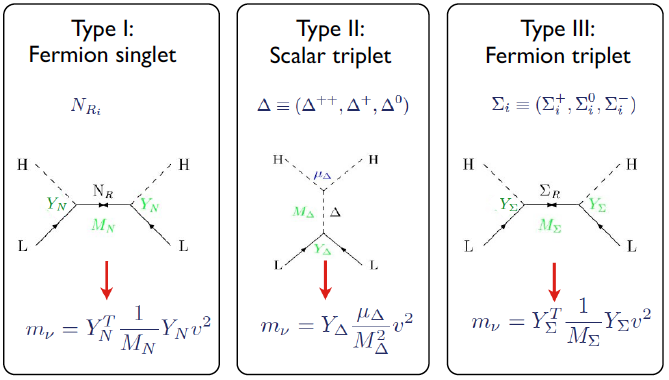
\includegraphics[width=0.7\textwidth]{images/seesaw.png}
\caption{New particles introduced in seesaw models (Passemar, 2015)}
\label{}
\end{figure}

\begin{figure}[h]
\centering
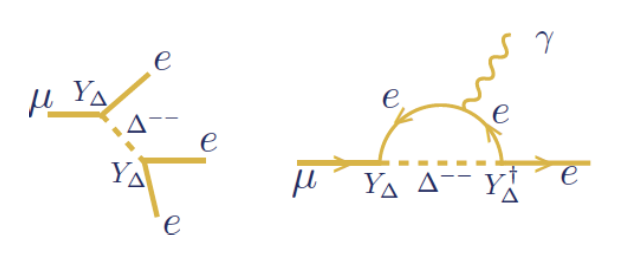
\includegraphics[width=0.5\textwidth]{images/seesaw-lfv-modes.png}
\caption{Scalars introduced in Type-II seesaw models mediating LFV decays (Passemar, 2015)}
\label{}
\end{figure}




\subsection{$\htm$ excess}

Hints of LFV can come in the form of experimental results which are not consistent with the SM. One such ``anomaly’’ is the $\htm$ excess. In 2015, CMS found a $2.4\sigma$ excess in the branching fraction of $\htm$ \cite{CMS:2015a}. This process is lepton flavour violating, so in the SM its branching fraction is expected to be consistent with zero. However it was determined

\begin{equation}
\br(h\to \tau \mu) = (0.84^{+0.39}_{-0.37})\%
\end{equation}


Also in 2015 was a similar search performed by ATLAS \cite{ATLAS:2015}, in which an excess of $1.2\sigma$ was found in the $\htm$ decay. 

\begin{equation}
B(\htm) = (0.77 \pm 0.66)\%
\end{equation}

Though this $1.2\sigma$ result is less indicative of NP, it still provides hints as to where NP could occur. These results indicate possible new physics in the Higgs sector! Several models, including Two-Higgs Doublet Models (2HDM), introduce new Higgs-like particles; these particles can couple with leptons to allow lepton flavour violating processes \cite{Harnik:2012}. In fact, LFV can occur naturally in any model with more than one Higgs doublet.


\begin{figure}[h]
\centering
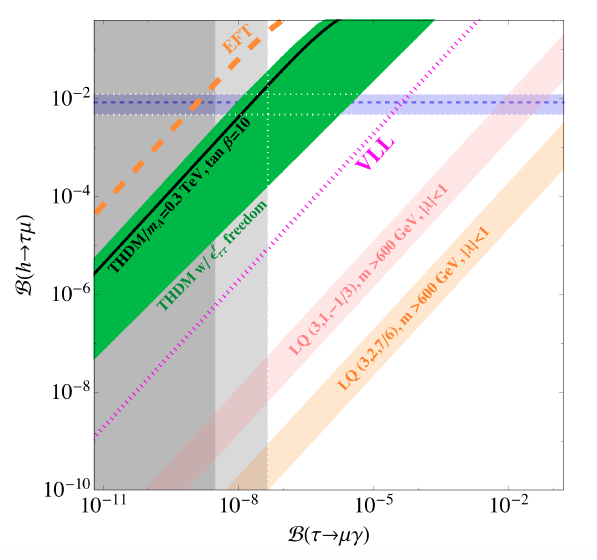
\includegraphics[width=0.7\textwidth]{images/h-vs-tau.png}
\caption{Correlation between $\br(\htm)$ and $\br(\tmg)$ in various NP scenarios (Dorsner et al., 2015)}
\label{}
\end{figure}


The present experimental result for $\br(\htm)$ is shown in horizontal blue band; current and future projections for $\br(\tmg)$ experimental sensitivity are represented with vertical light and dark gray bands. We note that certain 2HDM models predict a branching fraction for $\br(\tmg)$, consistent with the CMS results, at sensitivities which could be observed by Belle II. It is important to note that the Higgs sector could contribute to LFV in NP scenarios, and that both theory and experimental limits on other LFV processes such as $\htm$ all interweave with limits on $\tlg$ branching fractions to provide information on NP, even just through reducing the available phase space for certain models \cite{Dorsner:2015}.

\begin{figure}[h]
\centering
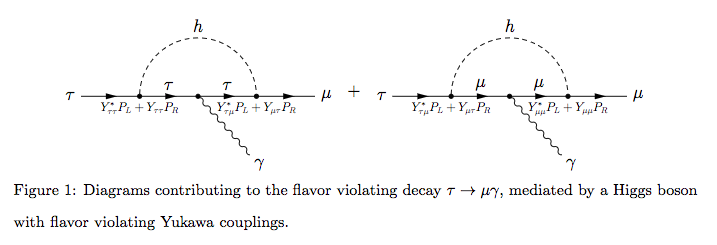
\includegraphics[width=0.9\textwidth]{images/higgs-lfv-modes.png}
\caption{Diagrams contributing to $\tmg$ decay, mediated by a Higgs boson with flavour violating Yukawa coupling (Harnick et al., 2012)}
\label{}
\end{figure}

As seen in Figure above, new Higgs particles can mediate LFV processes and allow for measurable amounts of LFV beyond the Standard Model \cite{Dorsner:2015}.


\subsection{Models predicting $\tlg$}

As mentioned previously, LFV in the $\tau$ sector is introduced in many NP scenarios as a consequence of generating neutrino mass (and hence facilitating neutrino mixing). Branching fractions of the modes $\tlg$ are highly calculable - there is little theoretical uncertainty.

\begin{figure}[h]
\centering
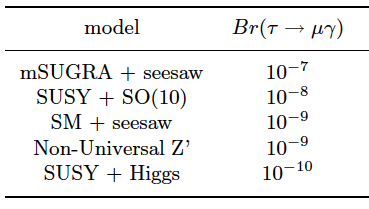
\includegraphics[width=0.5\textwidth]{images/np-models-bounds.png}
\caption{Upper limits of branching fractions from $\tmg$, predicted by models of new physics beyond the SM (various sources)\cite{Ohshima:2007zz}}
\label{}
\end{figure}

Figure above lists a few NP models with their predictions of $\br(\tmg)$. We see that the phase space of some of these models has already been ruled out with our current experimental limits on LFV branching fractions.



\section{Searches for $\tlg$}

The most recent searches for $\tlg$ were undertaken at Belle (2007) and Babar (2010), for both $\ell=\mu,e$ modes. These detectors are $e^+ e^-$ colliders; a signal of the form $e^+ e^-\to \tau^+ \tau^-$, with one tau (signal-side) decaying $\tau\to \ell \gamma$ and the other tau (tag-side) decaying generically, with the requirement that the tag-side track is not $\ell$.

The dominant backgrounds for the process $\tmg$ are $\tau\to \mu \nu \nu$, $\tau\to \pi \nu$ and $e^+ e^- \to \mu^+ \mu^- \gamma$ (with similar backgrounds for $\tau\to e \gamma$) \cite{Hayasaka:2007}. The first two backgrounds have branching fractions
\begin{align}
\br(\tau\to \mu \nu \nu)&=17.41\%\\
\br(\tau\to\pi\nu)&=10.83\%
\end{align}
which are non-negligible contributions to the dataset. The cross-section for we can compare the cross section of $e^+ e^- \to \mu^+ \mu^- \gamma$ to that of $e^+ e^- \to \tau^+ \tau^- \gamma$;
\begin{align}
\sigma(e^+ e^- \to \mu^+ \mu^- \gamma)&=\SI{0.242}{nb}\\
\sigma(e^+ e^- \to \tau^+ \tau^- \gamma)&=\SI{0.919}{nb}\\
\end{align}
so we note a significant contribution from this background also.

\begin{figure}[h]
\centering
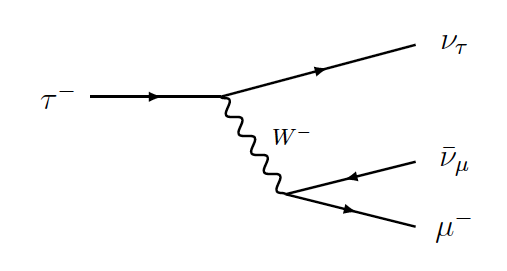
\includegraphics[width=0.3\textwidth]{images/taumununu.png}
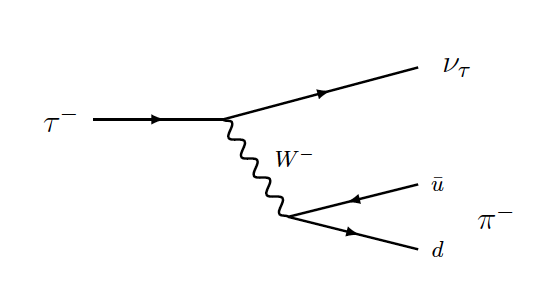
\includegraphics[width=0.3\textwidth]{images/taupinu.png}
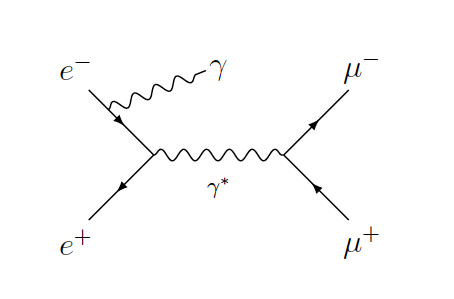
\includegraphics[width=0.3\textwidth]{images/eemumugamma.png}
\caption{Dominant backgrounds to $\tmg$. From left-to-right: $\tau\to \mu \nu \nu$, $\tau\to \pi \nu$ and $e^+ e^- \to \mu^+ \mu^- \gamma$}
\end{figure}


\subsection{Belle searches}


The Belle detector records events from an asymmetric $e^+ e^-$ collider with electron (positron) energy of $\SI{8}{GeV}$ ($\SI{3.5}{GeV}$). A detailed discussion of the detector can be found at Ref. \cite{Belle:2002}. In 2007, the Belle Collaboration performed a search over $\SI{535}{fb^{-1}}$ of $e^+ e^-$ data and set constraints \cite{Hayasaka:2007} on $\tlg$ branching fractions as

\begin{align}
\br(\tmg)&<\num{4.5d-8},\\
\br(\tau\to e \gamma)&<\num{1.2d-7}.
\end{align}


\subsection{Babar searches}

Similar to Belle, the Babar detector records events from an asymmetric $e^+e^-$ collider, with electron (positron) energy of $\SI{9}{GeV}$ ($\SI{3.1}{GeV}$). A detailed discussion of the detector can be found at Ref. \cite{Babar:2002}. The most recent search for $\tlg$ was performed in 2010 by the Babar Collaboration \cite{Babar:2010}, over a $\SI{515.5}{fb^{-1}}$ dataset, setting constraints on $\tlg$ branching fractions as

\begin{align}
\br(\tmg)&<\num{4.4d-8},\\
\br(\tau\to e \gamma)&<\num{3.3d-8}.
\end{align}



\section{Future searches}

\subsection{Belle II}

To probe smaller branching fractions for signals of new physics, we are required to build particle detectors with greater total integrated luminosity. The Belle II experiment, the successor to the Belle experiment, has a predicted total integrated luminosity of $\SI{50}{ab^{-1}}$. As a point of comparison, the Belle experiment collected $\SI{1000}{fb^{-1}}$ of data over its lifetime. A detailed discussion on the Belle II detector can be found at Ref \cite{Belle:2010}.

\begin{figure}[h]
\centering
%\includegraphics[width=0.9\textwidth]{images/tauLFV.png}
\caption{Current and future sensitivities on $\tau$ LFV branching fractions (Urquijo, 2016)}
\end{figure}

Increased luminosity will allow the branching fractions of various LFV processes to be probed with greater sensitivity. Figure above gives an indication of how future searches at Belle II will improve upper limits on the branching fractions for decays such as, importantly, $\tlg$.

\pagebreak

%-------------------------------------------------------------------

\chapter{The Belle and Belle II detectors}

The Belle experiment ...

Located in Tsukuba, Japan, the KEKB particle accelerator was used for the Belle experiment from 1999 to 2010 and collided high energy electrons and positrons of $\SI{8}{GeV}$ and $\SI{3.5}{GeV}$ respectively. Over its lifetime, the Belle detector collected a total time-integrated luminosity of $\SI{1000}{fb^{-1}}$, corresponding to ???? tau-pair events (from which our signal mode could occur).

The key components of the detector are the silicon vertex detector (SVD), the central drift chamber (CDC), the electromagnetic calorimeter (ECL), the time-of-flight/Cerenkov aerogel chamber (TOP), and the K-long/muon detector (KLM).

\begin{figure}[h]
\centering
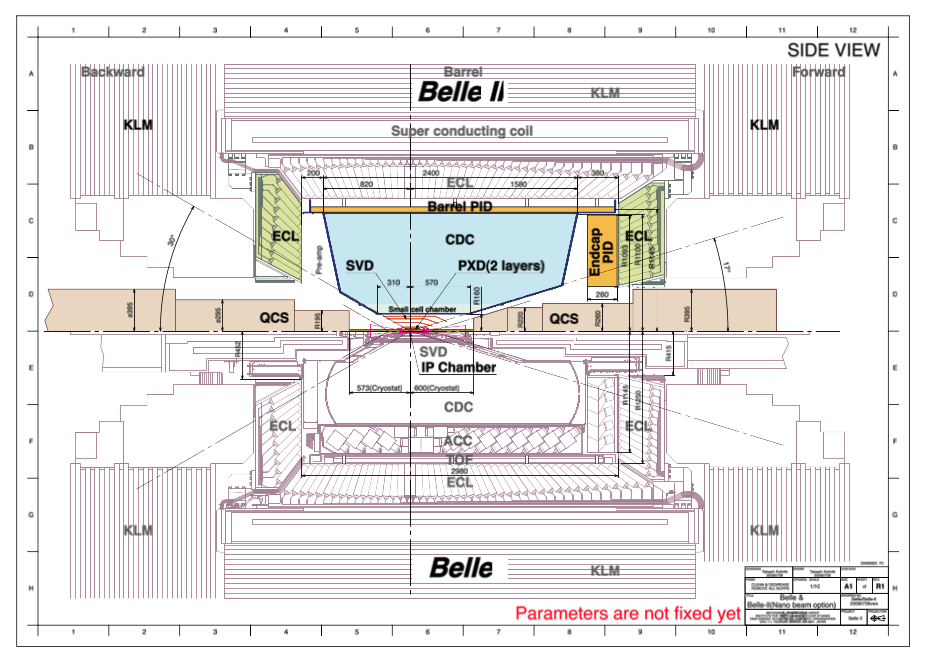
\includegraphics[width=0.8\linewidth]{images/super-kekb-side-view.png}
\caption{Super-KEKB detector design, side-view}
\label{}
\end{figure}

%-------------------------------------------------------------------


\section{Silicon Vertex Detector}


%-------------------------------------------------------------------


\section{Central Drift Chamber}

%-------------------------------------------------------------------


\section{Electromagnetic Calorimeter}

I can talk about the importance of cluster timing

\url{https://docs.belle2.org/record/344/files/BELLE2-NOTE-TE-2016-006.pdf}

%-------------------------------------------------------------------


\section{Time-of-flight/Cerenkov aerogel chamber}

%-------------------------------------------------------------------


\section{K-long/muon detector}


%-------------------------------------------------------------------


\section{Particle identification (PID)}


These PID values are generated through combination of many components of the detector, and provide the probability of a track being a particular particle. Due to how reconstruction is handled by the \texttt{reconstructDecay} module, some tracks may be double counted or misreconstructed. To account for this, several tighter PID cuts are implemented later.

%-------------------------------------------------------------------




\section{Super-KEKB}

The KEKB detector is currently undergoing upgrades to facilitate the running of the sequel to the Belle experiment, inventively labelled Belle II. The upgraded detector is known as Super-KEKB, and has a range of improvements over its predecessor. The SVD is being upgraded to include 6 layers (up from ???) which will allow for SOMETHING. Additionally, a Pixel Detector (PXD) is being installed around the interaction point, prior to the SVD, which will allow for even greater tracking of particle trajectories.

Over the course of the experiment, it is projected that Belle II will generate a total time-integrated luminosity of $\SI{50}{ab^{-1}}$, or $\SI{50000}{fb^{-1}}$; that is, 50 times more available data than with Belle.

The electron and positron beam energies differ from those used at Belle, with electron beam energy of $\SI{7.5}{GeV}$ (HER?) and positron beam energy (LER?) of $\SI{4}{GeV}$. This produces a center-of-mass energy of $\SI{11}{GeV}$.


\pagebreak


\section{Beam backgrounds}

SEE TECHNICAL DESIGN REPORT

Beam background is an important issue in B factories, and especially so for the upgraded energies of Super-KEKB. Key sources of this beam background are synchrotron radiation (SR), beam-gas scattering, and Touschek radiation.

Scattered particles and radiation photons, generated by these processes, collide with the beam pipe and generate showers of photons, leptons and hadronic particles. Additionally, other particles can be generated at the interaction point in the collision between opposite beams; these are mostly electron-positron pairs. These particles then interact with the detector, and are called beam background. This background can make searches for actual physics events difficult, due to the large number of clusters and tracks introduced.

\subsection{Synchrotron radiation}

As beam particles are bent by magnets while travelling through the accelerator, they emit synchrotron radiation.

\subsection{Beam-gas scattering}	

Inside the beam pipes is not a perfect vacuum; the designed gas pressure for Super-KEKB is $\SI{e-7}{Pa}$. Most of this gas is composed of neutral H$_2$ and CO$_2$. Beam particles can collide with the gas molecules, resulting in elastic scattering where energy is maintained by direction is changed (Coulomb scattering), or inelastic scattering whereby a photon is emitted from the scattered particle (bremsstrahlung).

\begin{figure}[h]
\centering
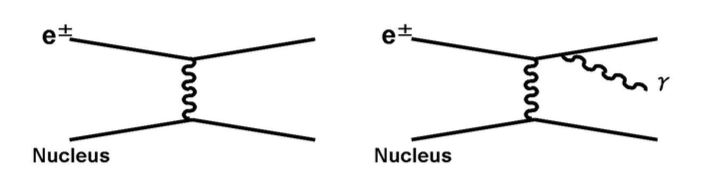
\includegraphics[width=\linewidth]{images/beam-gas-scattering.png}
\caption{Beam-gas scattering}
\label{fig:test2}
\end{figure}


\subsubsection{Coulomb scattering}

Beam electrons (or positrons) can elastically scatter off beam gas particles, changing direction such that the scattered particle does not reach the interaction point.

\subsubsection{Bremsstrahlung}

Beam-gas scattering can also occur as bremsstrahlung, where electrons (or positrons) recoil off gas nuclei and emit photons (see figure XXXX b) above). The photon carries away for fraction of the scattered particle's energy.


\subsection{Touschek scattering}

Particle beams do not exist as continuous ``lines'' of electrons and positrons marching through the accelerator in single file. Instead, we have tightly packed beam bunches, containing $10^{10} - 10^{11}$ particles each. In Super-KEKB the bunches have a designed cross-section perpendicular to the beam trajectory of XXXXX, up from XXXXX in KEKB (LENGTH??). These bunches are aligned almost perfectly parallel so that beam particles do not collide with the beam pipe during their many cycles around the accelerator.

Within these bunches the particles oscillate in a direction perpendicular to the beam trajectory, so that in addition to interacting with beam-gas, particles within a beam bunch collide with each other resulting in an transfer of energy and momentum. Trajectories of these particles may be changed by this interaction, so that they do not reach the interaction point. 

\begin{figure}[h]
\centering
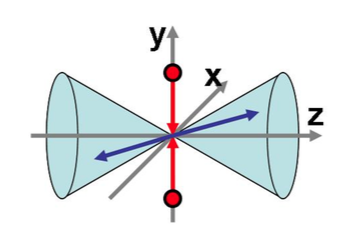
\includegraphics[width=0.5\linewidth]{images/touschek-beam-frame.png}
\caption{An illustration of Touschek scattering in the bunch frame}
\label{fig:test2}
\end{figure}



\pagebreak
%-------------------------------------------------------------------

\chapter{Monte Carlo production and background types}

Electron-positron collisions at Belle II will produce a wide range of different physics events. Within these, we hope to find the signal modes $\tau\to\mu\gamma$ and $\tau\to e\gamma$. Many other events, known as ``background'' events, will.....

In this analysis, we investigate all generically decaying tau-pair processes, mu-pair events ($e^+ e^- \to \mu^+ \mu^- (\gamma)$), bhabha scattering ($e^+ e^- \to e^+ e^- \gamma$), qqbar continuum (where $q = u, d, c, s$), and generic B$\bar{\text{B}}$ continuum ($e^+ e^- \to B^+ B^-$ and $e^+ e^- \to B^0 \bar{B}^0$). Of the tau-pair processes, we specifically investigate the modes $\tau^{\pm} \to \mu^{\pm} \nu \nu$, $\tau^{\pm} \to e^{\pm} \nu \nu$, and $\tau^{\pm} \to \pi^{\pm} \nu$, as these are expected to be dominant backgrounds.

We investigate the characteristic signals of observables such as momentum, energy, and polar angles (object trajectory relative to collision axis ???) as well as other constructed variables, in simulated data known as Monte Carlo (MC). By looking at signal and background signals separately in MC, we are able discriminate between signal and background events in data (NO I don't actually do this.... feasibility test? Not sure how to describe why I do what I do and what it accomplishes).

\section{Event generation}

All MC was generated in the Belle II Analysis Framework (\texttt{basf2}) with Belle II (Super-KEKB) geometry and energies. HOW DOES GENERATION HAPPEN? 

The geometry of the detector is accurately known by the generators, which includes very specific location, thickness and material information; magnetic field strength through the detector is also known. The detector components are simulated by the generator, so that timing information and energy deposition is recorded for these components as MC particles interact with them. Following the simulation of a physics event, information from the sub-detectors is used to reconstruct ``tracks'' (correponding to charged particles) and ``clusters'' (referring to cells of the ECL with which a particle has interacted with, corresponding to photons).

Signal MC was produced using the \texttt{KKMC} generator (REF PHILL'S GENERATOR PAPER). Decays proceeded as $e^+ e^- \to \tau^+ \tau^-$, with one tau decaying to the signal mode $\tau \to \ell \gamma$ (the ``signal'' side), and the other (the ``tag'' side) decaying to all experimentally measured SM decay modes of the tau, scaled by their branching ratio; decaying according to the SM is referred to ``generic'' decay. The modes $\tau^+ \to \ell^+ \gamma$, $\tau^-$ decaying generically, and $\tau^- \to \ell^- \gamma$, $\tau^+$ decaying generically were both generated so that differences were not overlooked. To investigate both the electron and muon modes, two distinct final states were produced. The number of produced events was 3,100,000 for the muon final state, and 3,550,000 for the electron final state.

Samples for a range of background events were produced by the Belle II Collaboration. 


\section{Event scaling}

The full Belle II dataset is expected to have a time-integrated luminosity of $\SI{50}{ab^{-1}}$ (UM HMM what do I do here). Instead of running over the equivalent amount of background events expected in such a sample size, we can run over a smaller number of events then scale our results. This is done for computing reasons, as the number of background events recorded for these luminosities quickly becomes prohibitively large.

We choose to scale up to a luminosity of $\SI{1000}{fb^-1}$; this is the total time-integrated luminosity of the complete Belle dataset, and so is useful as a point of comparison to previous searches. The scale factor for each event type is calculated by

\begin{equation}
n_{\SI{1000}{fb^{-1}}} = n_{\text{generated}} \times \text{scale factor},
\end{equation}

where $n_{\SI{1000}{fb^{-1}}}$ = $\mathcal{L} \sigma$, and $n_{\text{generated}}$ is the number of events generated. Scaled event numbers are presented in Table XXXX below.

\begin{table}[h]
\centering
\begin{tabular}{lllll}
\textbf{Event type} & $\mathbf{n_{\text{generated}}}$ & $\mathbf{n_{\SI{1000}{fb^{-1}}}}$ & 
\textbf{scale factor}\\\hline
\rowcolor[HTML]{EFEFEF} 
$\tau \to \mu\gamma$ & \num{3.1d6} & 82.71 & \num{2.66806d-5}\\
\rowcolor[HTML]{EFEFEF} 
$\tau \to e\gamma$ & \num{3.55d6} & 220.56 & \num{6.21296d-5} \\       
$\tau \to \mu\nu\nu$ & ?? & \num{3.19996d8} & 9.99987\\
$\tau \to \pi\nu$ & \num{38d6} & \num{1.99055d8} & 5.2383 \\
$\tau \to e\nu\nu$ & ?? & \num{3.27715d8} & 68.274 \\
$\tau \to \text{generic}$ & ?? & ?? & 15.7339  \\
$e^+e^- \to \mu^+\mu^-(\gamma)$ & \num{681d6} & \num{1.148d9} & 1.68576 \\
$e^+e^- \to e^+e^-\gamma$ & \num{71.52d6} & \num{3d11} & 4194.63 \\
$e^+e^- \to u\bar{u}$ & \num{d6} & \num{1.61d9} & 1610 \\
$e^+e^- \to d\bar{d}$ & \num{d6} & \num{4d8} & 400 \\
$e^+e^- \to c\bar{c}$ & \num{d6} & \num{1.3d9} & 1300 \\
$e^+e^- \to s\bar{s}$ & \num{d6} & \num{3.8d8} & 380 \\
$e^+e^- \to B^+B^-$ & \num{d6} & \num{1.2d9} & 1200 \\
$e^+e^- \to B^0\bar{B}^0$ & \num{d6} & \num{1.2d9} & 1200
\end{tabular}
\caption{Scaled event numbers}
\label{my-label}
\end{table}

Unless explicitly stated, scaled event numbers will be used throughout this report (??? paper/thesis/document/analysis??) as to provide accurate points of comparison between events.


\section{Version differences}

The software framework on which event generation was performed is undergoing continuous development; a majority of signal and background MC was produced on the same release version to ensure accuracy between MC types. This version was made available on XXXXX, and was one of the most up-to-date releases at the time of analysis. However, the backgrounds $\mu^+\mu^-(\gamma)$ and $e^+ e^-(\gamma)$ (mu-pair and bhabha, respectively) did not have any events generated using this release, and instead used an older release dated XXXXX.

A full investigation into the differences in generated MC between releases has not been performed in this analysis, as it is assumed they are negligible in most relevant cases. Changes relate mostly to generation of beam backgrounds (??); however one major change is in the reporting of timing data from the ECL. From the release dated XXXX onwards, these associated times will be reported in nanoseconds, rather than uncalibrated clock ticks (REF). In comparing samples of signal MC generated in both the older and newer releases, figures XXXX a) and b) below, as well as private correspondance with the developer responsible for these changes, it was found that conversion to the newer scale could be made by adding 80 units to the cluster timing values.

   \begin{figure}[h]
        \centering
        \begin{subfigure}[b]{0.475\textwidth}
            \centering
            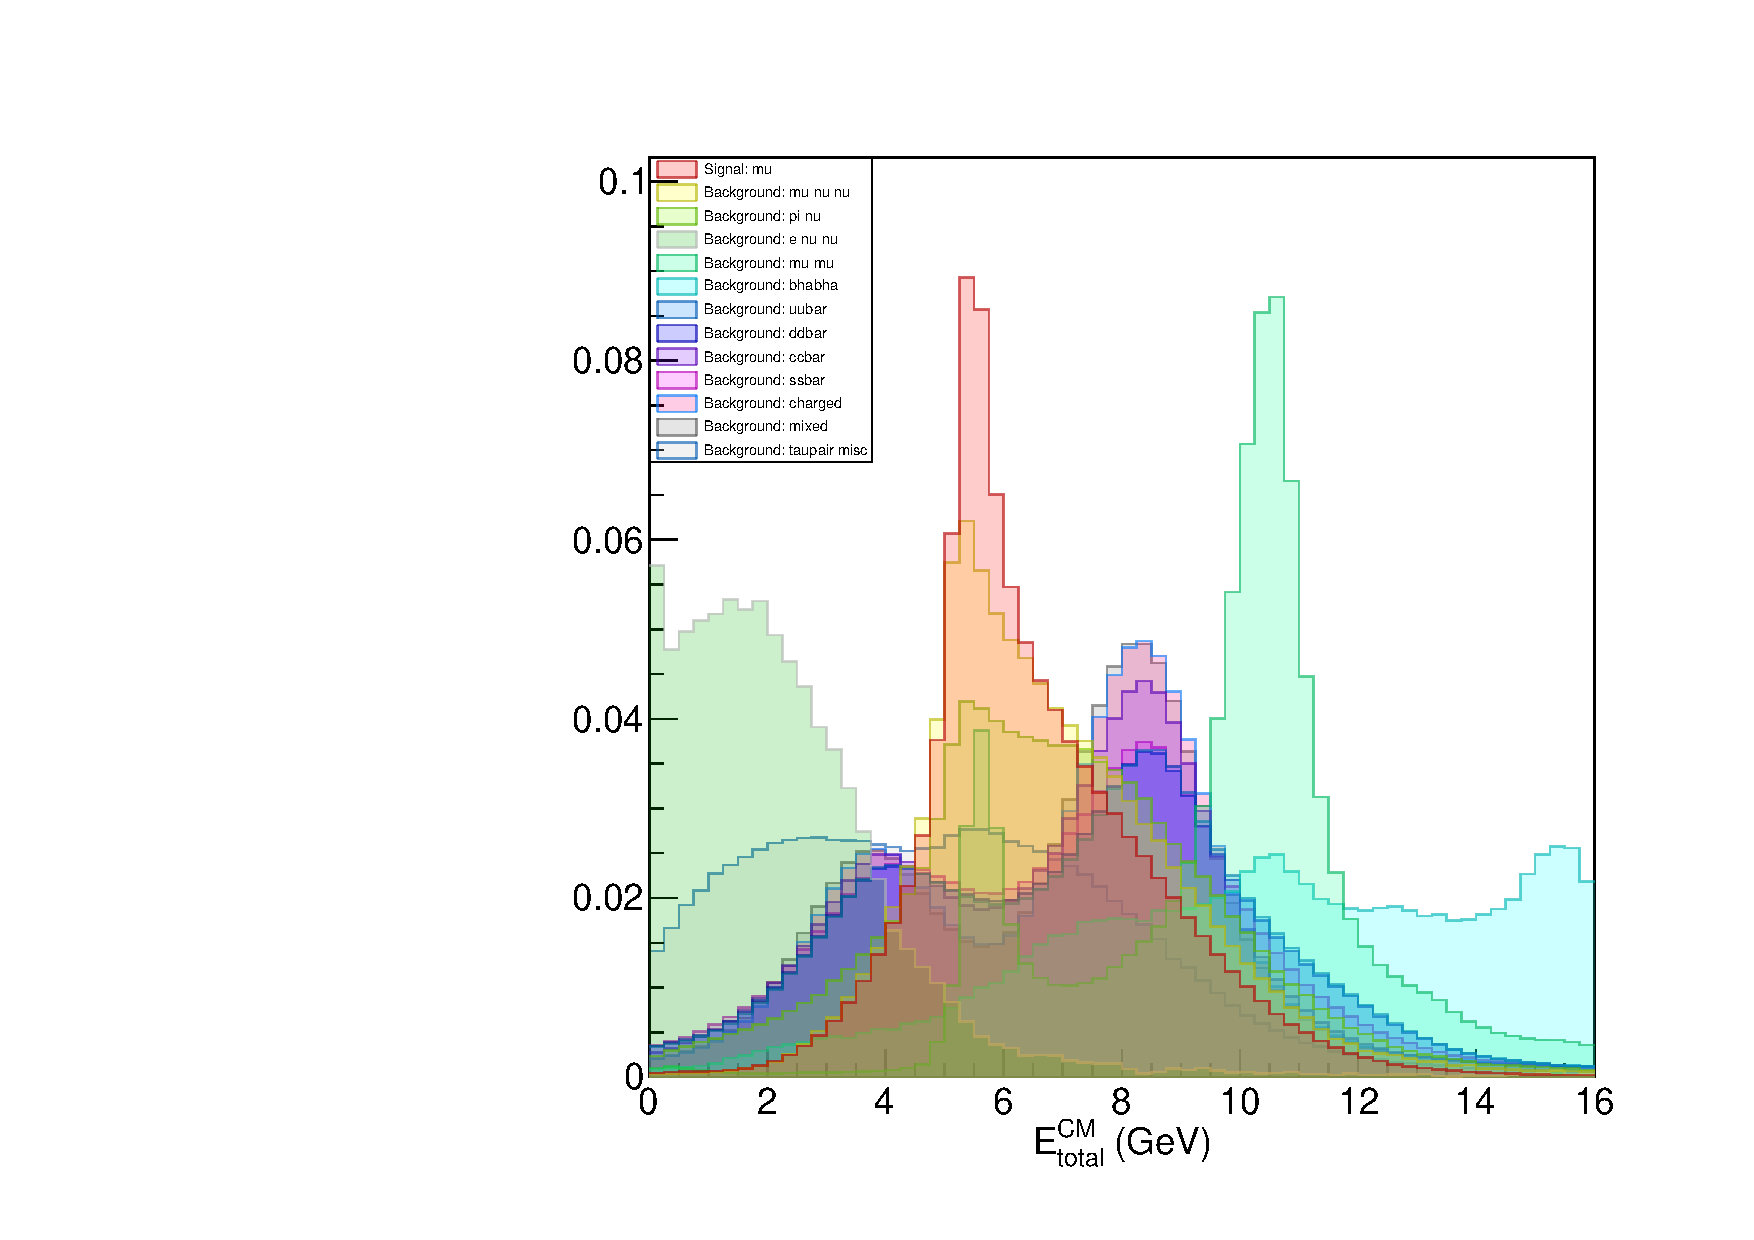
\includegraphics[width=\textwidth]{images/test.pdf}
            \caption[Network2]%
            {{\small Network 1}}    
            \label{fig:mean and std of net14}
        \end{subfigure}
        \hfill
        \begin{subfigure}[b]{0.475\textwidth}  
            \centering 
            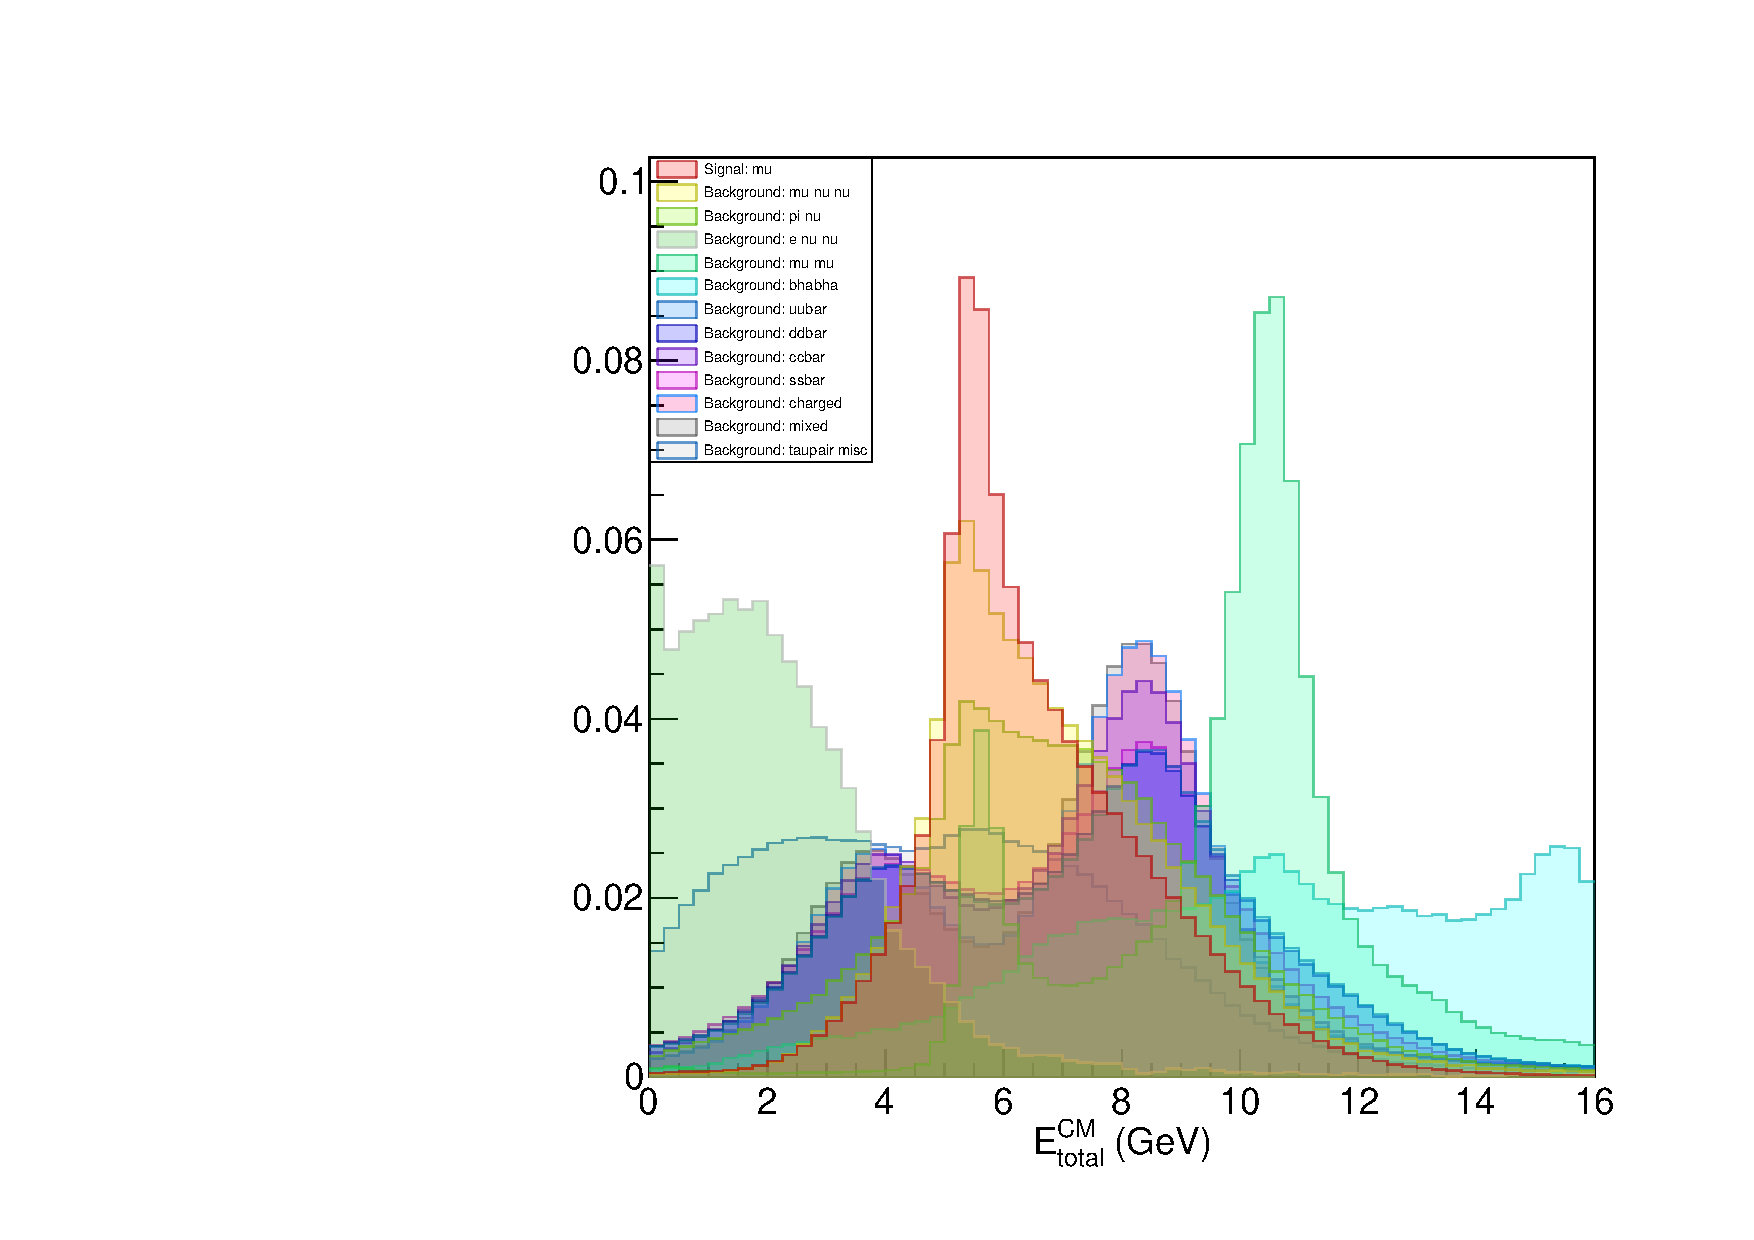
\includegraphics[width=\textwidth]{images/test.pdf}
            \caption[]%
            {{\small Network 2}}    
            \label{fig:mean and std of net24}
        \end{subfigure}
    \end{figure}



\section{Implementation of beam backgrounds}

Signal and background MC was generated with simulated beam background. To implement this beam background, several background components have been separately generated by the Belle II Collaboration. These are generated separately for the electron and positron beams and comprise four  types of beam backgrounds - large angle bhabha events, Coulomb scattering, Touschek scattering, and radiative bhabha.

For comparison, some samples of MC were generated without beam background. Comparisons between some measureables are shown in figures XXX, XXX, XXX below.

   \begin{figure}[h]
        \centering
        \begin{subfigure}[b]{0.475\textwidth}
            \centering
            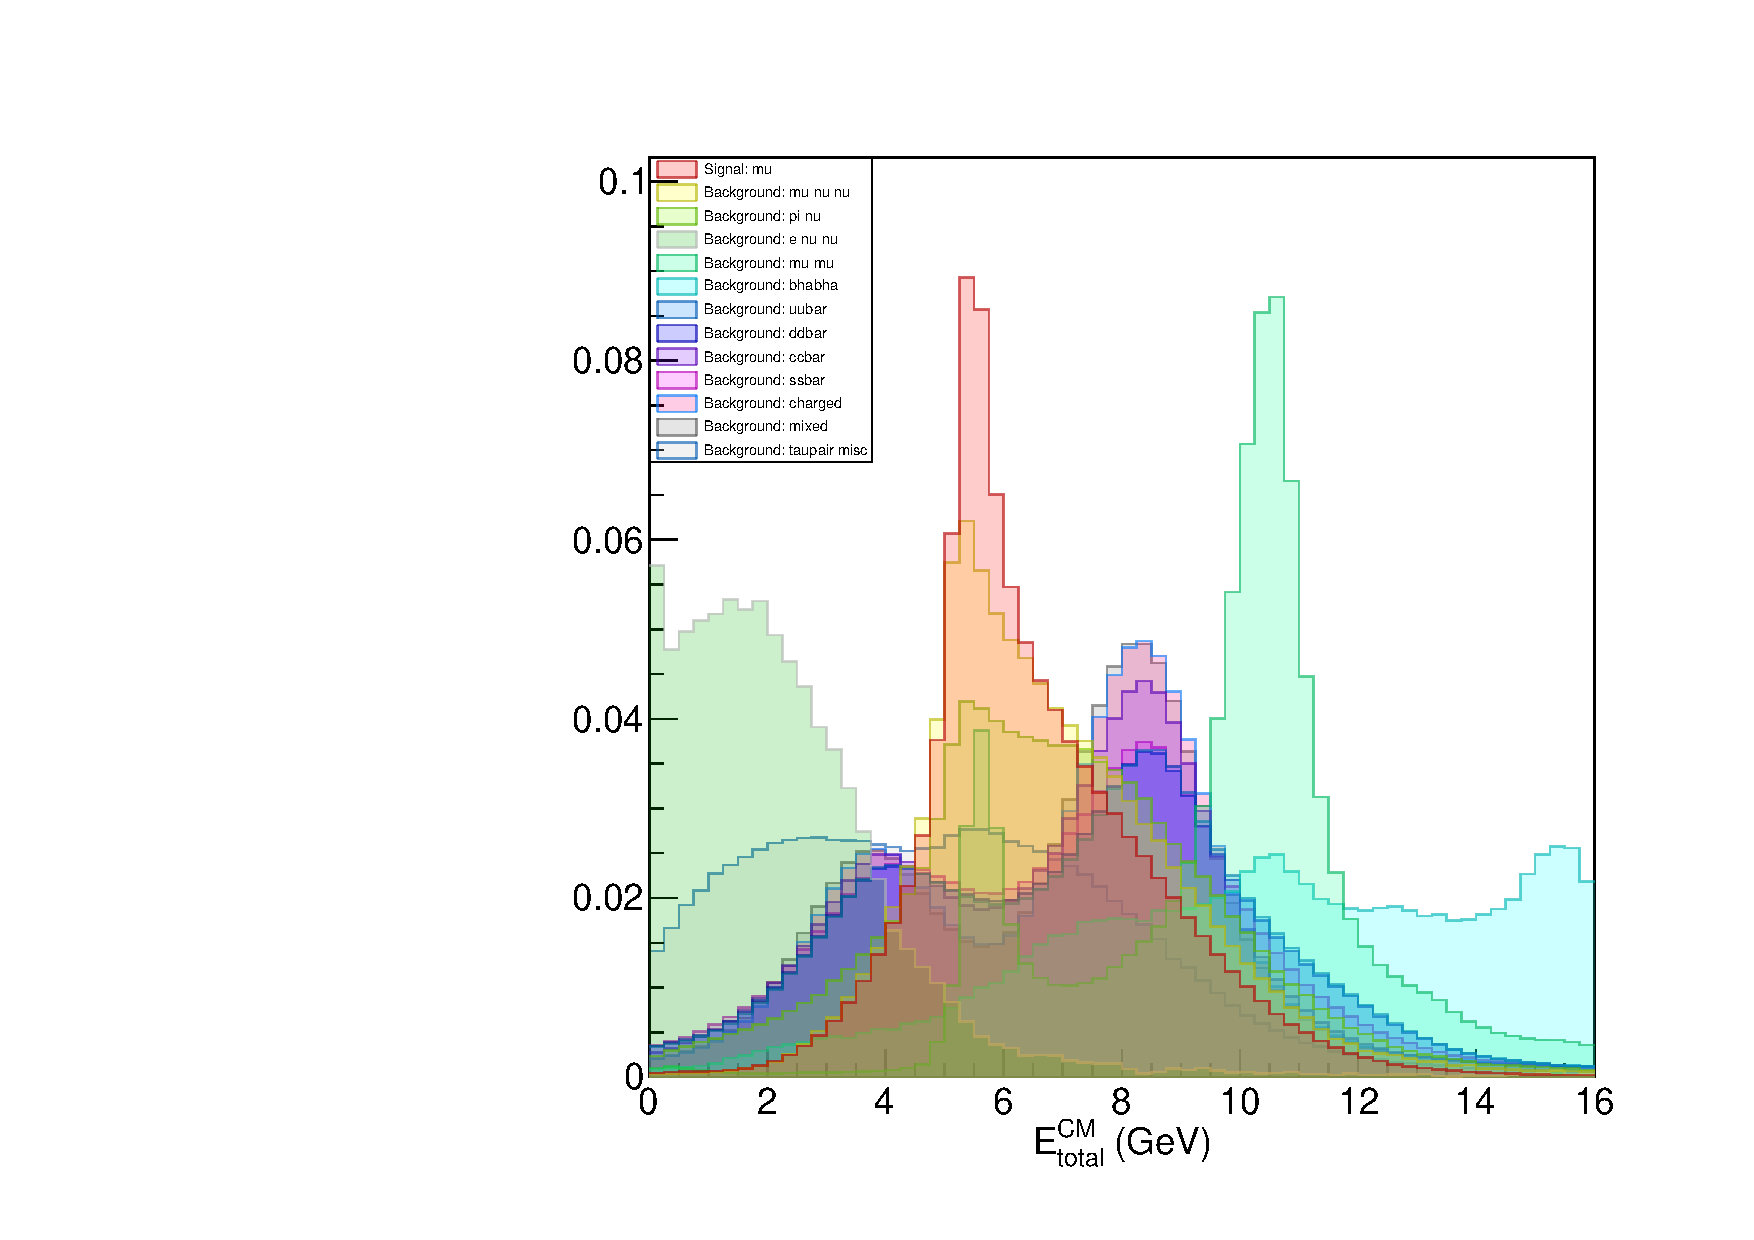
\includegraphics[width=\textwidth]{images/test.pdf}
            \caption[Network2]%
            {{\small Total center-of-mass energies w/o beam background}}    
            \label{fig:mean and std of net14}
        \end{subfigure}
        \hfill
        \begin{subfigure}[b]{0.475\textwidth}  
            \centering 
            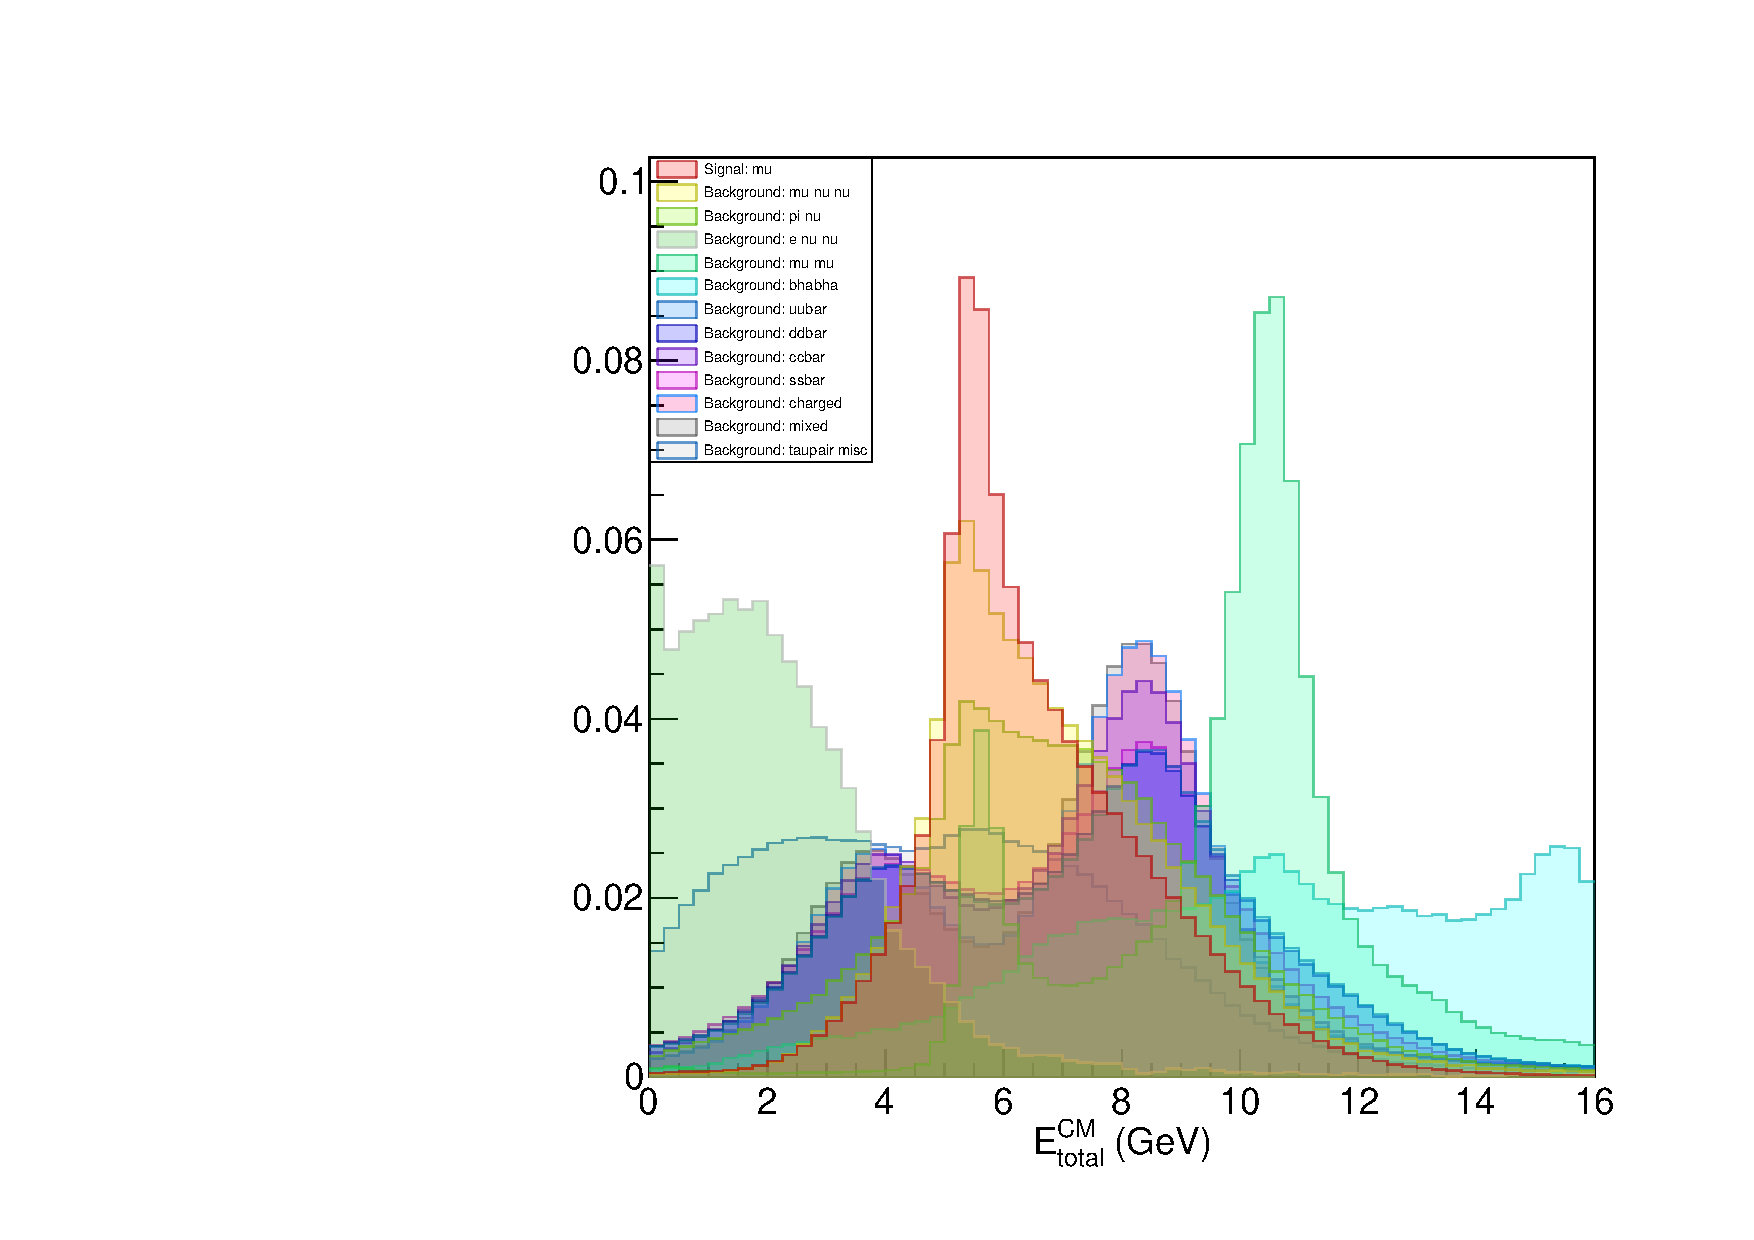
\includegraphics[width=\textwidth]{images/test.pdf}
            \caption[]%
            {{\small Total center-of-mass energies w/ beam background}}    
            \label{fig:mean and std of net24}
        \end{subfigure}
    \end{figure}
    
    
   \begin{figure}[h]
        \centering
        \begin{subfigure}[b]{0.475\textwidth}
            \centering
            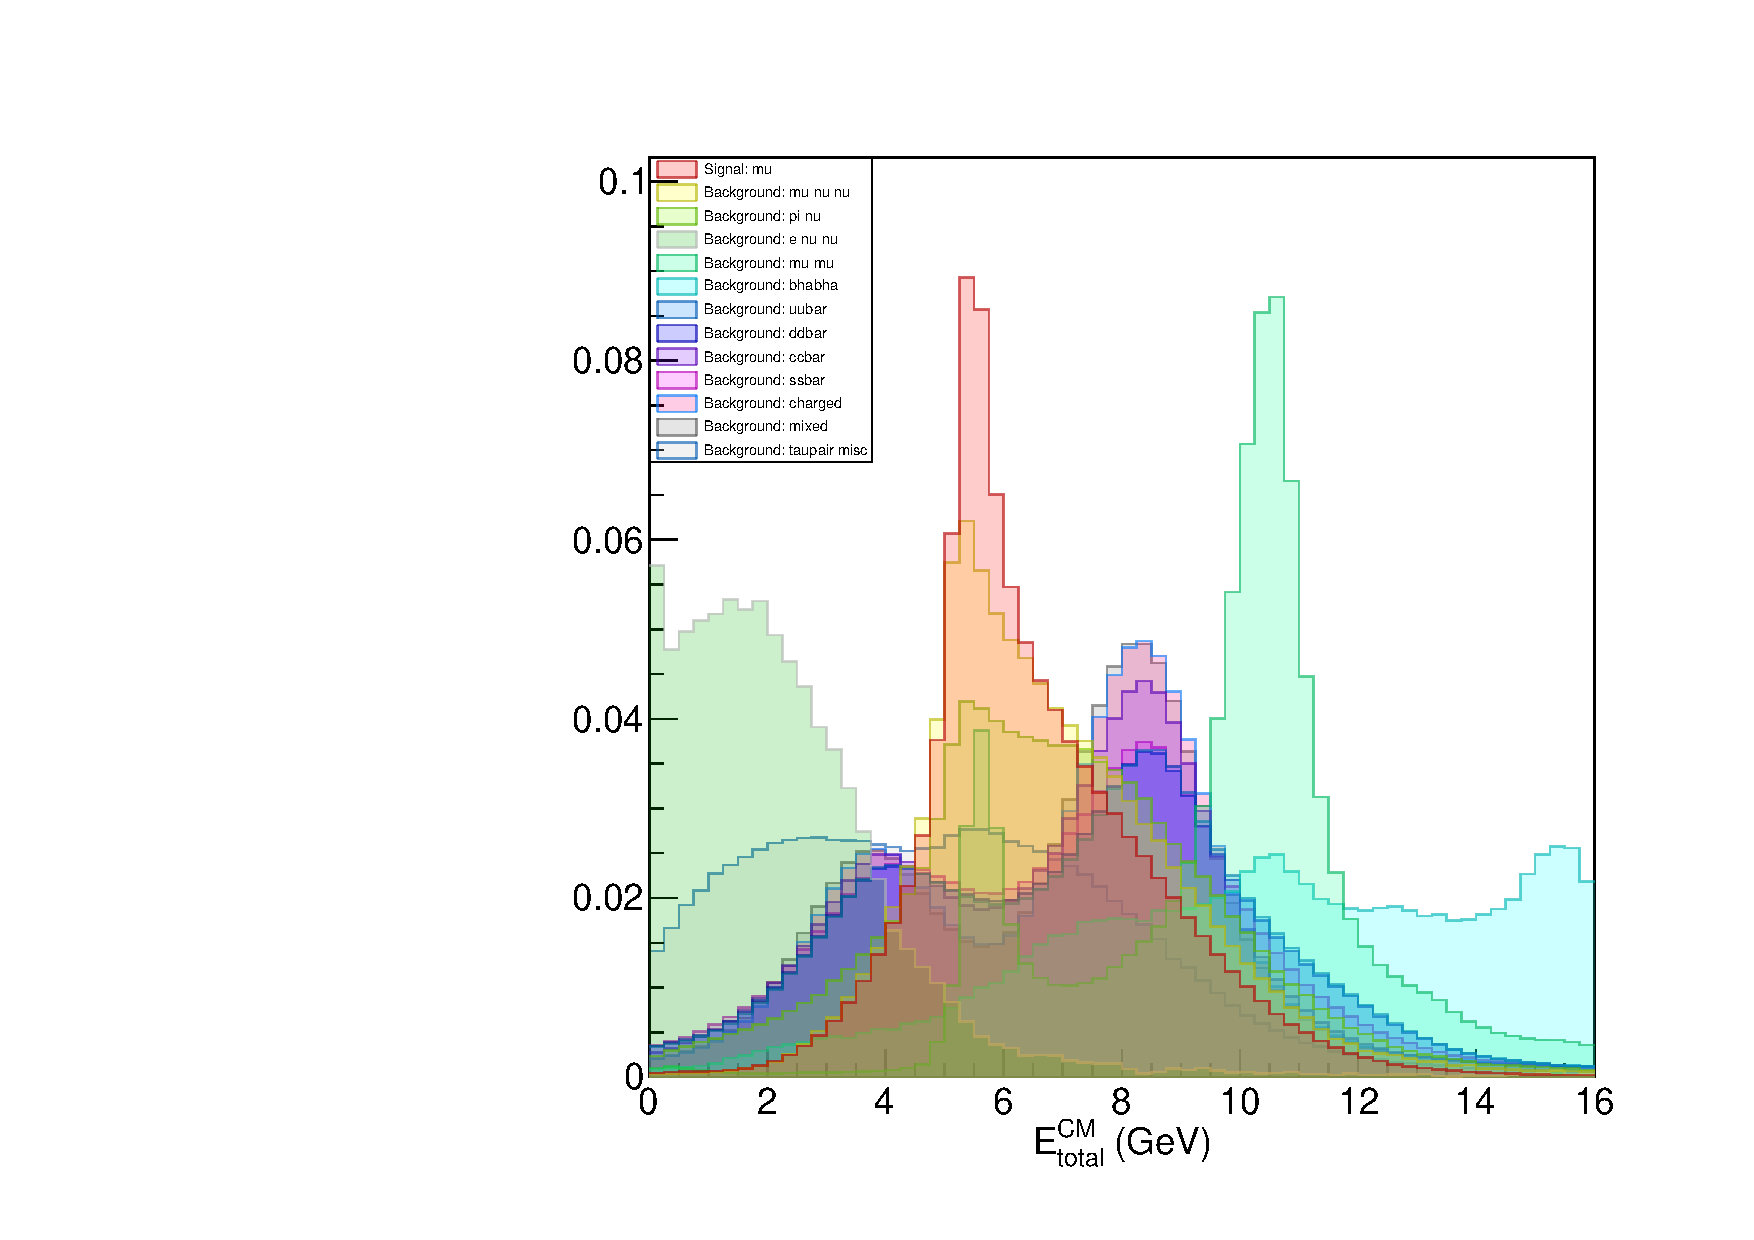
\includegraphics[width=\textwidth]{images/test.pdf}
            \caption[Network2]%
            {{\small Total center-of-mass energies w/o beam background}}    
            \label{fig:mean and std of net14}
        \end{subfigure}
        \hfill
        \begin{subfigure}[b]{0.475\textwidth}  
            \centering 
            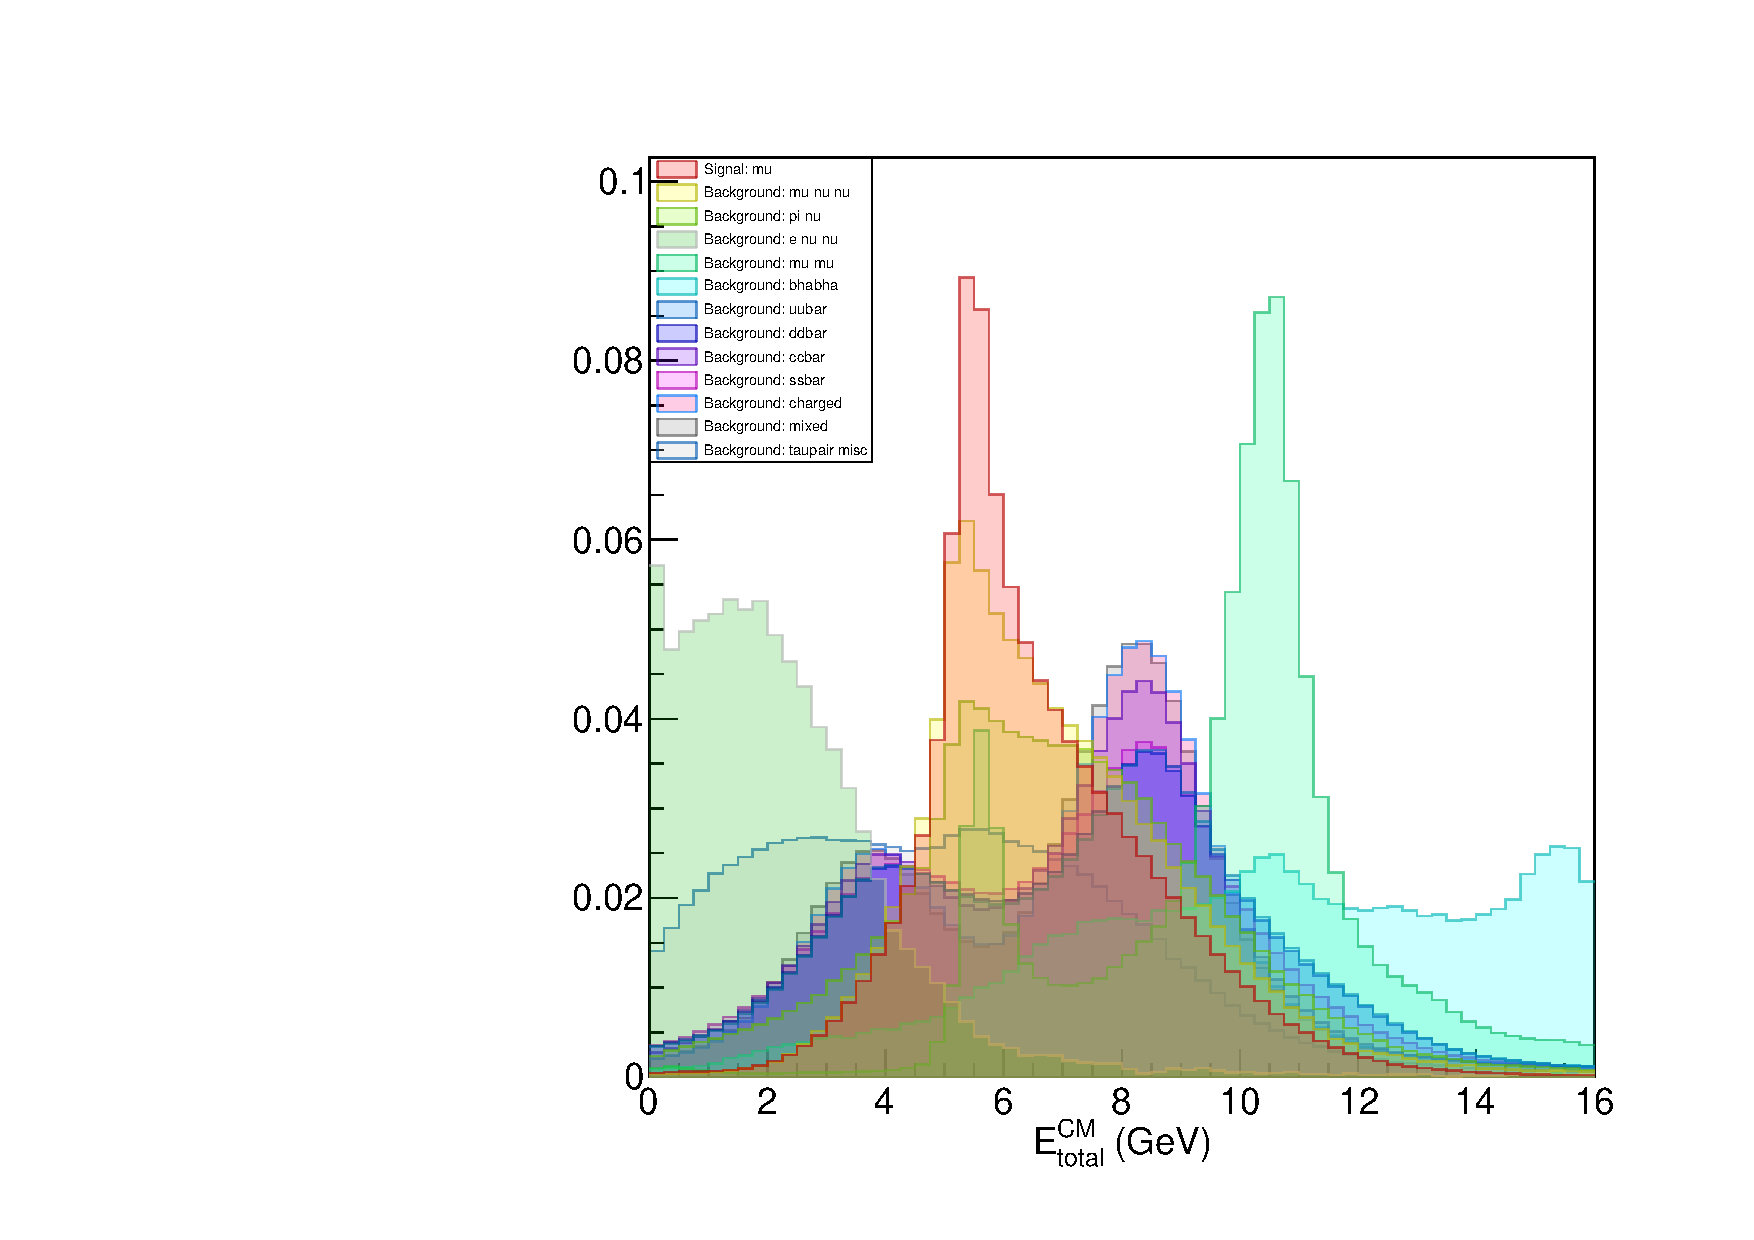
\includegraphics[width=\textwidth]{images/test.pdf}
            \caption[]%
            {{\small Total center-of-mass energies w/ beam background}}    
            \label{fig:mean and std of net24}
        \end{subfigure}
    \end{figure}
    
    
   \begin{figure}[h]
        \centering
        \begin{subfigure}[b]{0.475\textwidth}
            \centering
            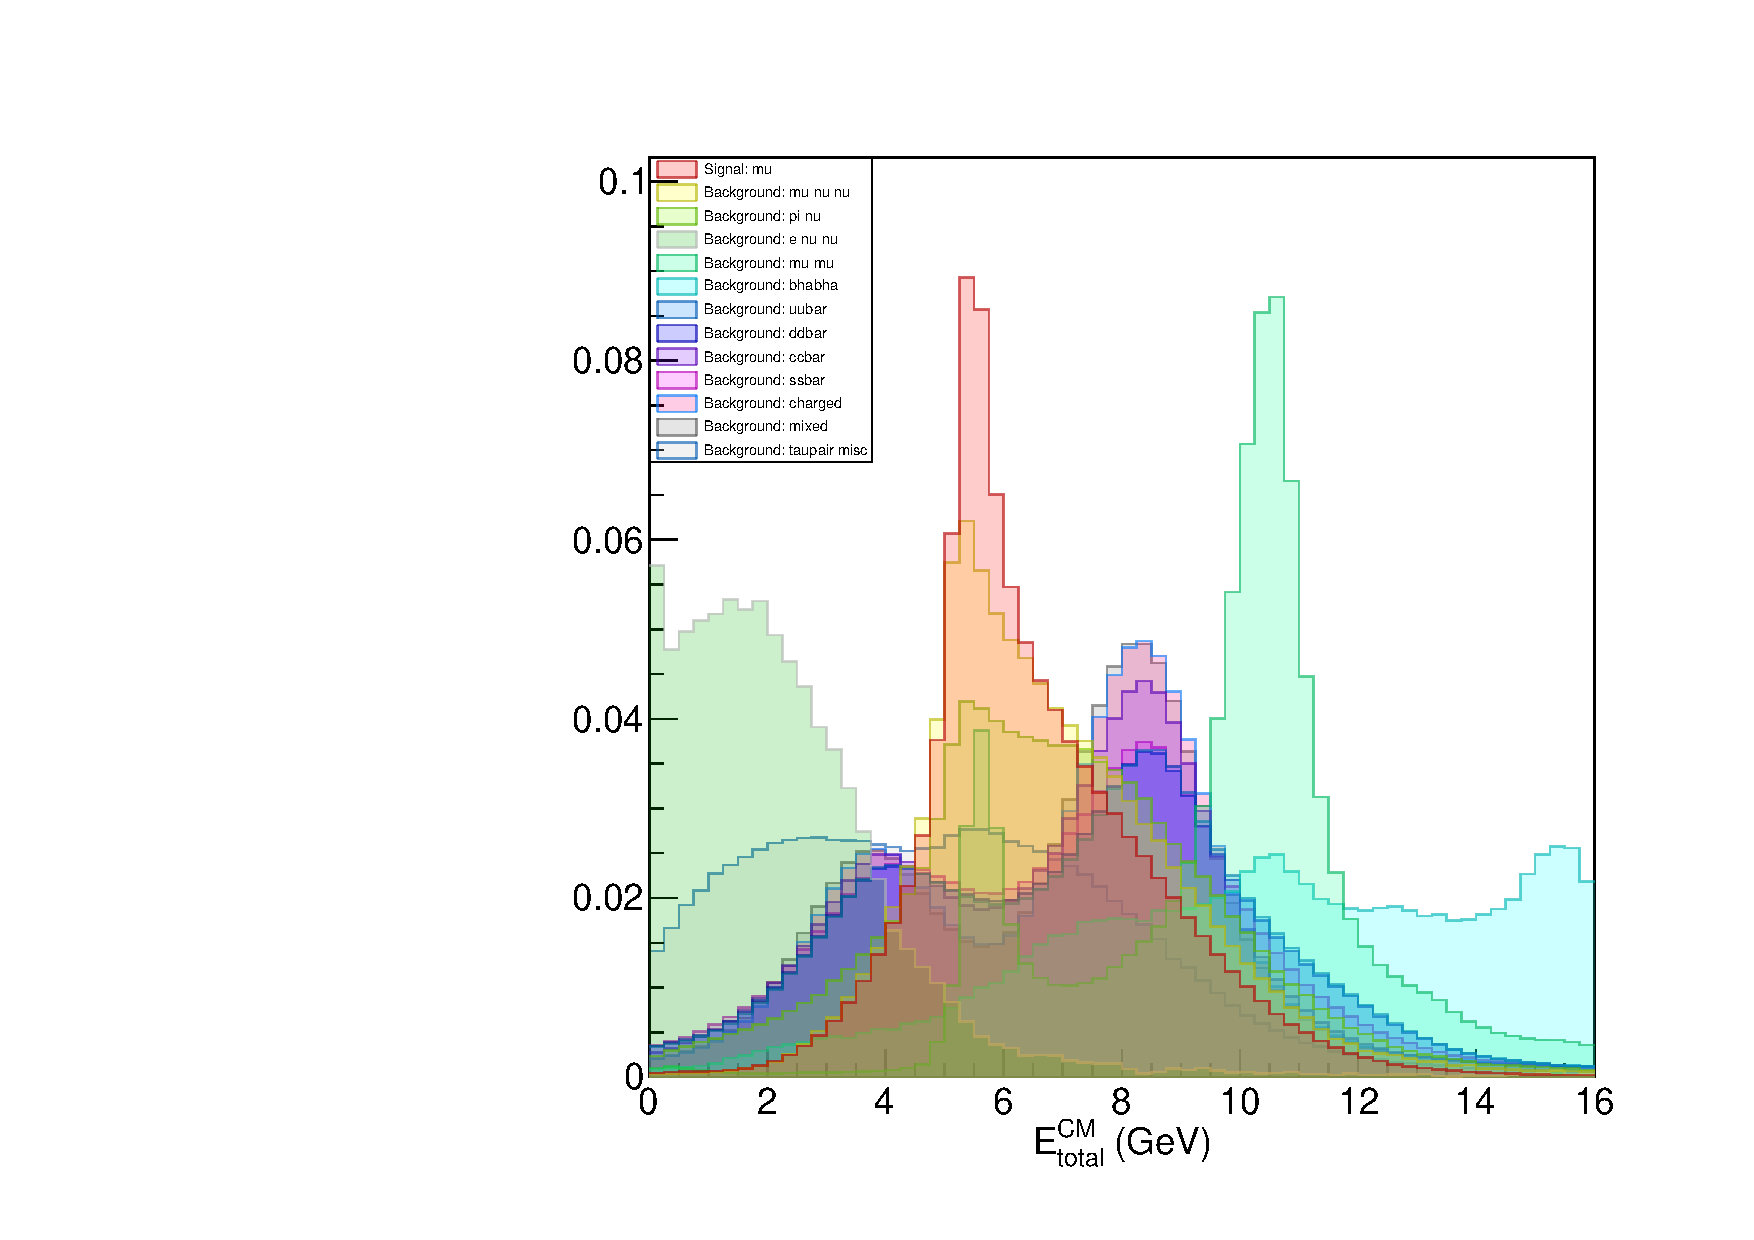
\includegraphics[width=\textwidth]{images/test.pdf}
            \caption[Network2]%
            {{\small Total center-of-mass energies w/o beam background}}    
            \label{fig:mean and std of net14}
        \end{subfigure}
        \hfill
        \begin{subfigure}[b]{0.475\textwidth}  
            \centering 
            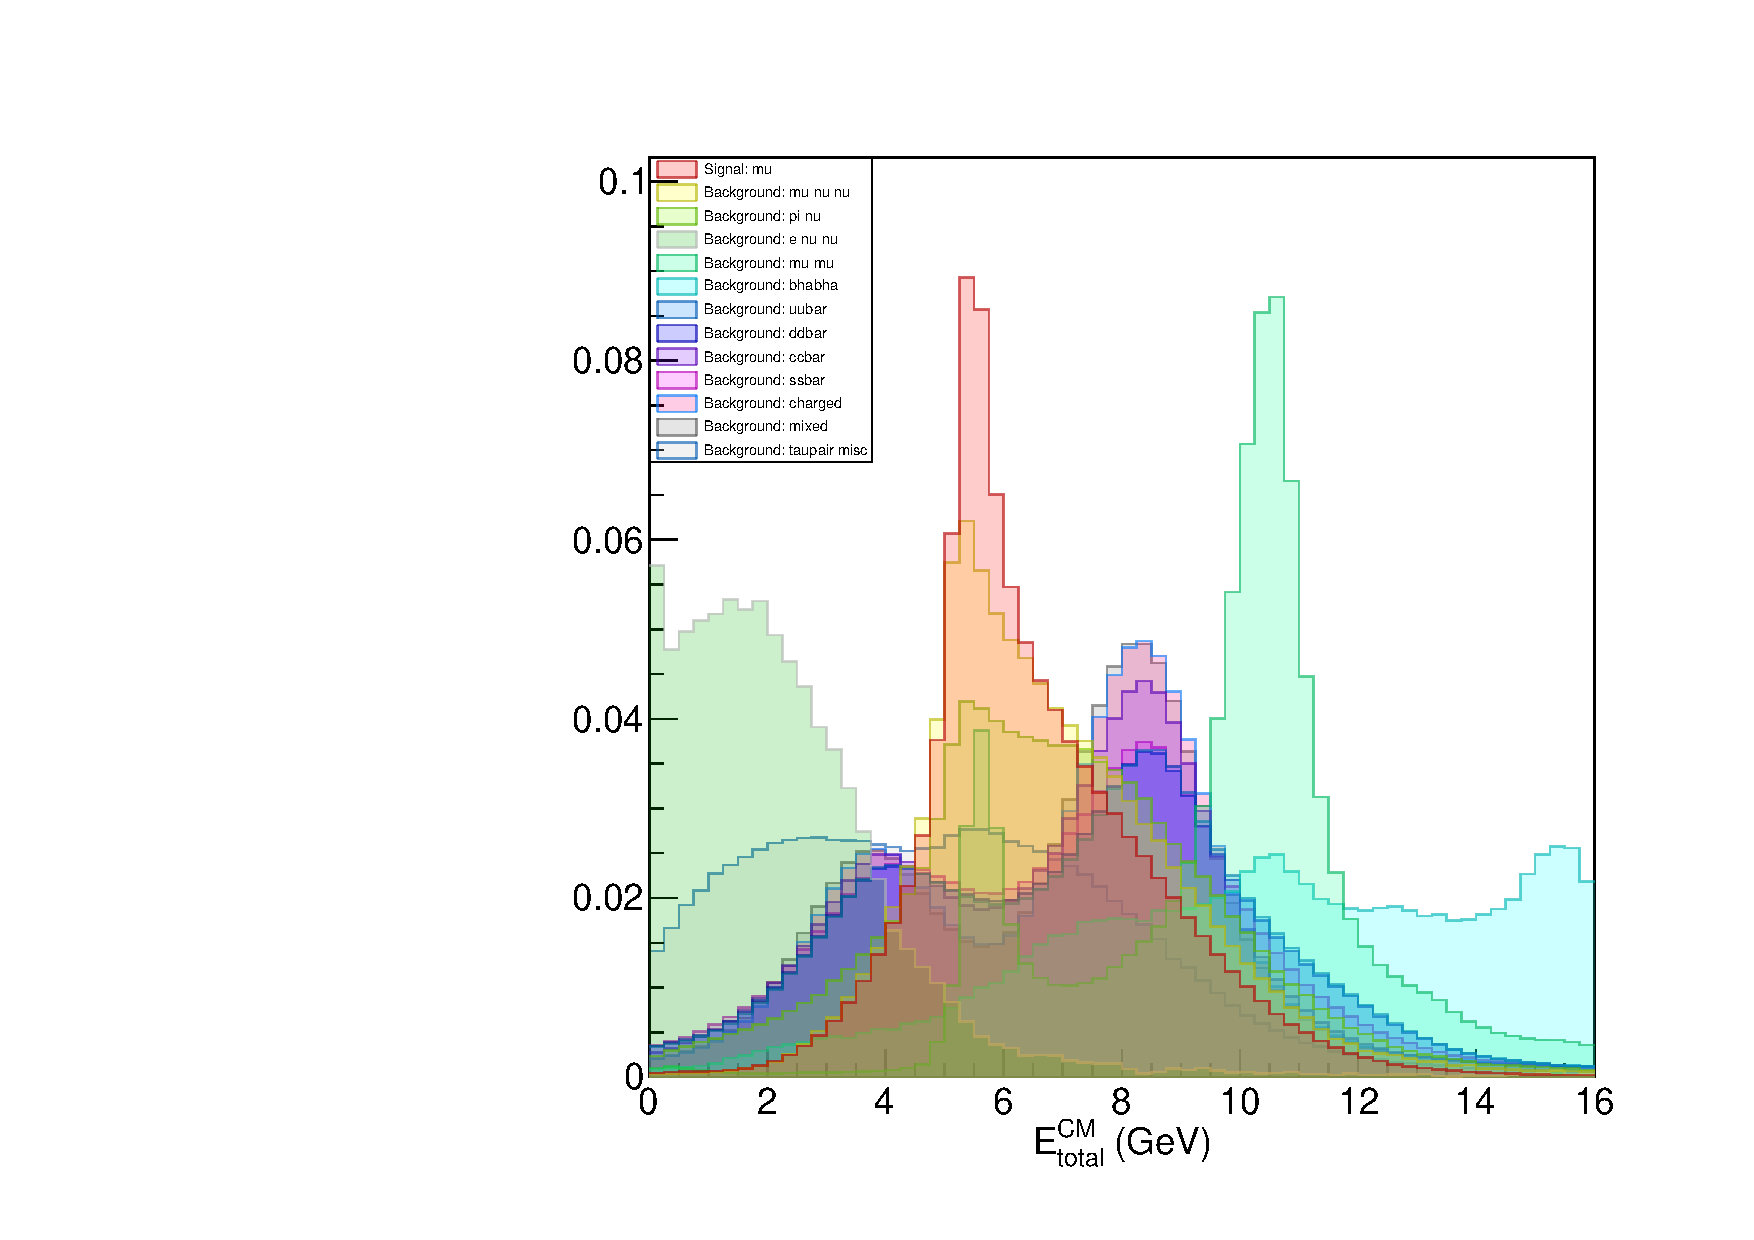
\includegraphics[width=\textwidth]{images/test.pdf}
            \caption[]%
            {{\small Total center-of-mass energies w/ beam background}}    
            \label{fig:mean and std of net24}
        \end{subfigure}
    \end{figure}
    
    
There are many differences between MC with and without beam background; only a few key points will be discussed here. Most obvious is the number of tracks recorded. Taking, for instance, our signal mode, we would expect for most events 2 or 4 tracks - one signal-side track corresponding to $\mu/e$, and one or three tracks on the tag-side (one- or three-pronged) coming from standard model $\tau$ decays, which are dominantly one- or three-pronged. Beam background particles in the detector produce a number of new tracks (as well as clusters) which are tracked by sub-detector components, then later reconstructed.

Kinematic variables such as energy and momentum are also obviously affected by beam background. We observe an increase in low energy and low momentum tracks; in these cases low energy beam background particles have been misidentified as signal- or tag-side particles originating from tau-pair processes.





\pagebreak
%------------------------------------------------------------------

\chapter{Reconstruction}

Reconstruction of events was performed through \texttt{basf2}. The generated MC consists of information about charged tracks travelling through the detector geometry and interacting with sub-detectors, as well as cluster information relating 
to photons from the ECL, among other information. 

To reconstruct events, we fill lists of particles by categorising tracks as specific charged particles - muons, electrons or pions, and by associating clusters with photons. These categorisations are performed with loose criteria to remove obvious background events. Tracks with PID values greater than 0.1 (or 0.5?) are considered muons, and similar for electrons and pions; the photon list is populated by clusters passing a ``goodness'' test. 



DISCUSS SIGNAL SIDE/TAG SIDE (+signal track, signal photon).


In the following, the \emph{signal track} describes the reconstructed track associated with the final state electron or muon from $\tau\to\ell\gamma$; similarly the \emph{signal photon} describes the cluster associated with the final state photon. These terms do not necessarily refer to the physical charged track or photon from the signal modes under analysis - 

The signal-side particles do not necessarily refer to the physical charged particle or photon coming from the signal modes under analysis; misidentified particles (such as a pion being identified as a muon during reconstruction) or particles from different decay processes (such as a muon from the tau process $\tau\to\mu\nu\nu$).


We reconstruct the signal side tau as $\tau \to \mu \gamma$ for the muon mode, or $\tau \to e \gamma$ for the electron mode. The tag side tau is reconstructed by requiring at least one muon, electron or charged pion. In addition to PID cuts, we also apply loose cuts to our $\Delta E$ and $M_{\text{inv}}$. We define our signal region variables as
\begin{align}
\Delta E &= E^{\text{CM}}_{\text{signal }\tau} - E_{\text{beam}}/2,\\
M_{\text{inv}} &= \text{invariant mass of reconstructed signal side tau},
\end{align}
where $E^{\text{CM}}_{\text{signal }\tau}$ is the center-of-mass energy of the reconstructed signal-side tau, and $E_{\text{beam}}$ is the total center-of-mass energy of the electron-positron beam system. Nominally we expect signal events to have $\Delta E\sim 0$ and $M_{\text{inv}}\sim m_{\tau}$; signal region selection is further discussed in Section XXXX.

Once background has been sufficiently reduced through use of selection criteria, signal candidates will be chosen from events in the $\Delta E$ vs. $M_{\text{inv}}$ phase space. As such we cut (???) only very loosely on these criteria wherever possible; in reconstruction we require $\SI{-0.4}{GeV} < \Delta E < \SI{0.2}{GeV}$ and $\SI{1.6}{GeV} < M_{\text{inv}} < \SI{1.9}{GeV}$ for the signal side tau. 

The number of events over which reconstruction was performed, as well as the percentage of events after reconstruction/events before reconstruction (which we shall call \emph{reconstruction efficiency} $\epsilon_{\text{recon}}$), is shown in TABLE XXXX below (I WANT TO REWORD THIS).

\begin{table}[h]
\centering
\begin{tabular}{llll}
\textbf{MC type}         & \textbf{events in (generated)} & \textbf{events out (reconstructed)} & $\mathbf{\epsilon_{\text{recon}}}$ \\ \hline 
\rowcolor[HTML]{EFEFEF} 
$\tau\to\mu\gamma$       & \num{3.1d6}        & 2914095             & 94.00\%                            \\
\rowcolor[HTML]{EFEFEF} 
$\tau\to e \gamma$      & \num{3.55d6}       & 3111190             & 87.64\%                            \\
$\tau\to\mu\nu\nu$      & ??                 & \num{32d6}          & ??                                 \\
$\tau\to\pi\nu$         & ??                 & \num{38d6}          & ??                                 \\
$\tau\to e\nu\nu$       & ??                 & \num{4.8d6}         & ??                                 \\
$\tau\to\text{generic}$  & ??                 & \num{63d6}          & ??                                 \\
$e^+ e^- \to \mu^+ \mu^- (\gamma)$       & \num{681d6}        & \num{16.9332d6}     & 2.487\%             \\
$e^+ e^- \to e^+ e^- \gamma$      & \num{71.52d6}      & \num{1.403d6}       & 1.455\%                            \\
$e^+ e^- \to u \bar{u}$       & \num{d6}           & 20794               & 0.2079\%                           \\
$e^+ e^- \to d \bar{d}$        & \num{d6}           & 20199               & 0.2020\%                           \\
$e^+ e^- \to c \bar{c}$        & \num{d6}           & 13688               & 0.1369\%                           \\
$e^+ e^- \to s \bar{s}$       & \num{d6}           & 15979               & 0.1598\%                           \\
$e^+ e^- \to B^+ B^-$     & \num{d6}           & 24907               & 0.2491\%                           \\
$e^+ e^- \to B^0 \bar{B}^0$       & \num{d6}           & 26058               & 0.2606\%                          
\end{tabular}
\caption{Reconstruction efficiency}
\label{my-label}
\end{table}


% A landscape table
\begin{sidewaystable}
\bigskip
\centering  
  \begin{tabular}{|l|l|l|l|l|l|p{2.5in}|}  
  \hline  
  \multicolumn{6}{|c|}{Text in columns 1 through 6}   
        & A paragraph 2.5 inches wide \\  
  \hline  
  Column 1 & Column 2 & Column 3 & Column 4 & Column 5 & Column 6
                      & This text is a paragraph.  It will wrap  
                      around to the next line if necessary. \\  
  Column 1 & Column 2 & Column 3 & Column 4 & Column 5 & Column 6
                      & The paragraph column \\  
  \hline  
  \end{tabular}  
  \caption{A Very Wide Table}  	
\end{sidewaystable}


\pagebreak


\chapter{Event topologies}

We discuss expected energies, kinematics and signal-side event topologies with comparison to MC data. Knowledge of event topologies is important in selecting regions in phase space to remove when optimising the ratio of signal-to-background. 

\section{Signal}

This also serves also validation of the signal MC - since it was generated and used by an individual rather than by multiple people within the Belle II Collaboration, the possibility of errors in generation and reconstruction are higher than for background MC. 


\subsection{Muon mode}

The mode $\tau\to\mu\gamma$ has a simple signal side, with only one track and one photon, and no missing energy (in the form of neutrinos). If we assume that on average both $\tau$ particles generated in the $e^+ e^-$ collision share equally the energy generated in the interaction, we expect the mean signal-side center-of-mass frame energy to be $\SI{5.5}{GeV}$. No physical preference is given to the energy distribution between the signal muon and signal photon, so their center-of-mass energies should be normally distributed around $\SI{2.75}{GeV}$. Recalling the relation between energy, momentum and mass,

\begin{equation}
E^2 = p^2 + m^2,
\end{equation}
since the muon energy is much greater than its mass of $\SI{105.66}{MeV/c^2}$ this can simplify to
\begin{equation}
E^2 \approx p^2.
\end{equation}

Note that $p$ is the magnitude of the particle's 3-momentum.

We can predict and compare with MC several topological measureables, such as polar angle (i.e. angle from an axis parallel to the beam trajectory) as well as opening angles between particles; this is done for several key measureables. The average opening angle between the signal muon and signal photon in the center-of-mass frame can be calculated by boosting the expected back-to-back pair from the signal $tau$ frame into the lab frame.

CALCULATIONS.

Similarly for SOME OTHER PAIRING,

CALCULATIONS.

As shown in figures XXXX below, the MC matches the predicted kinematics and topologies for the muon mode.


\begin{figure}[h]
\centering
\begin{minipage}{.5\textwidth}
  \centering
  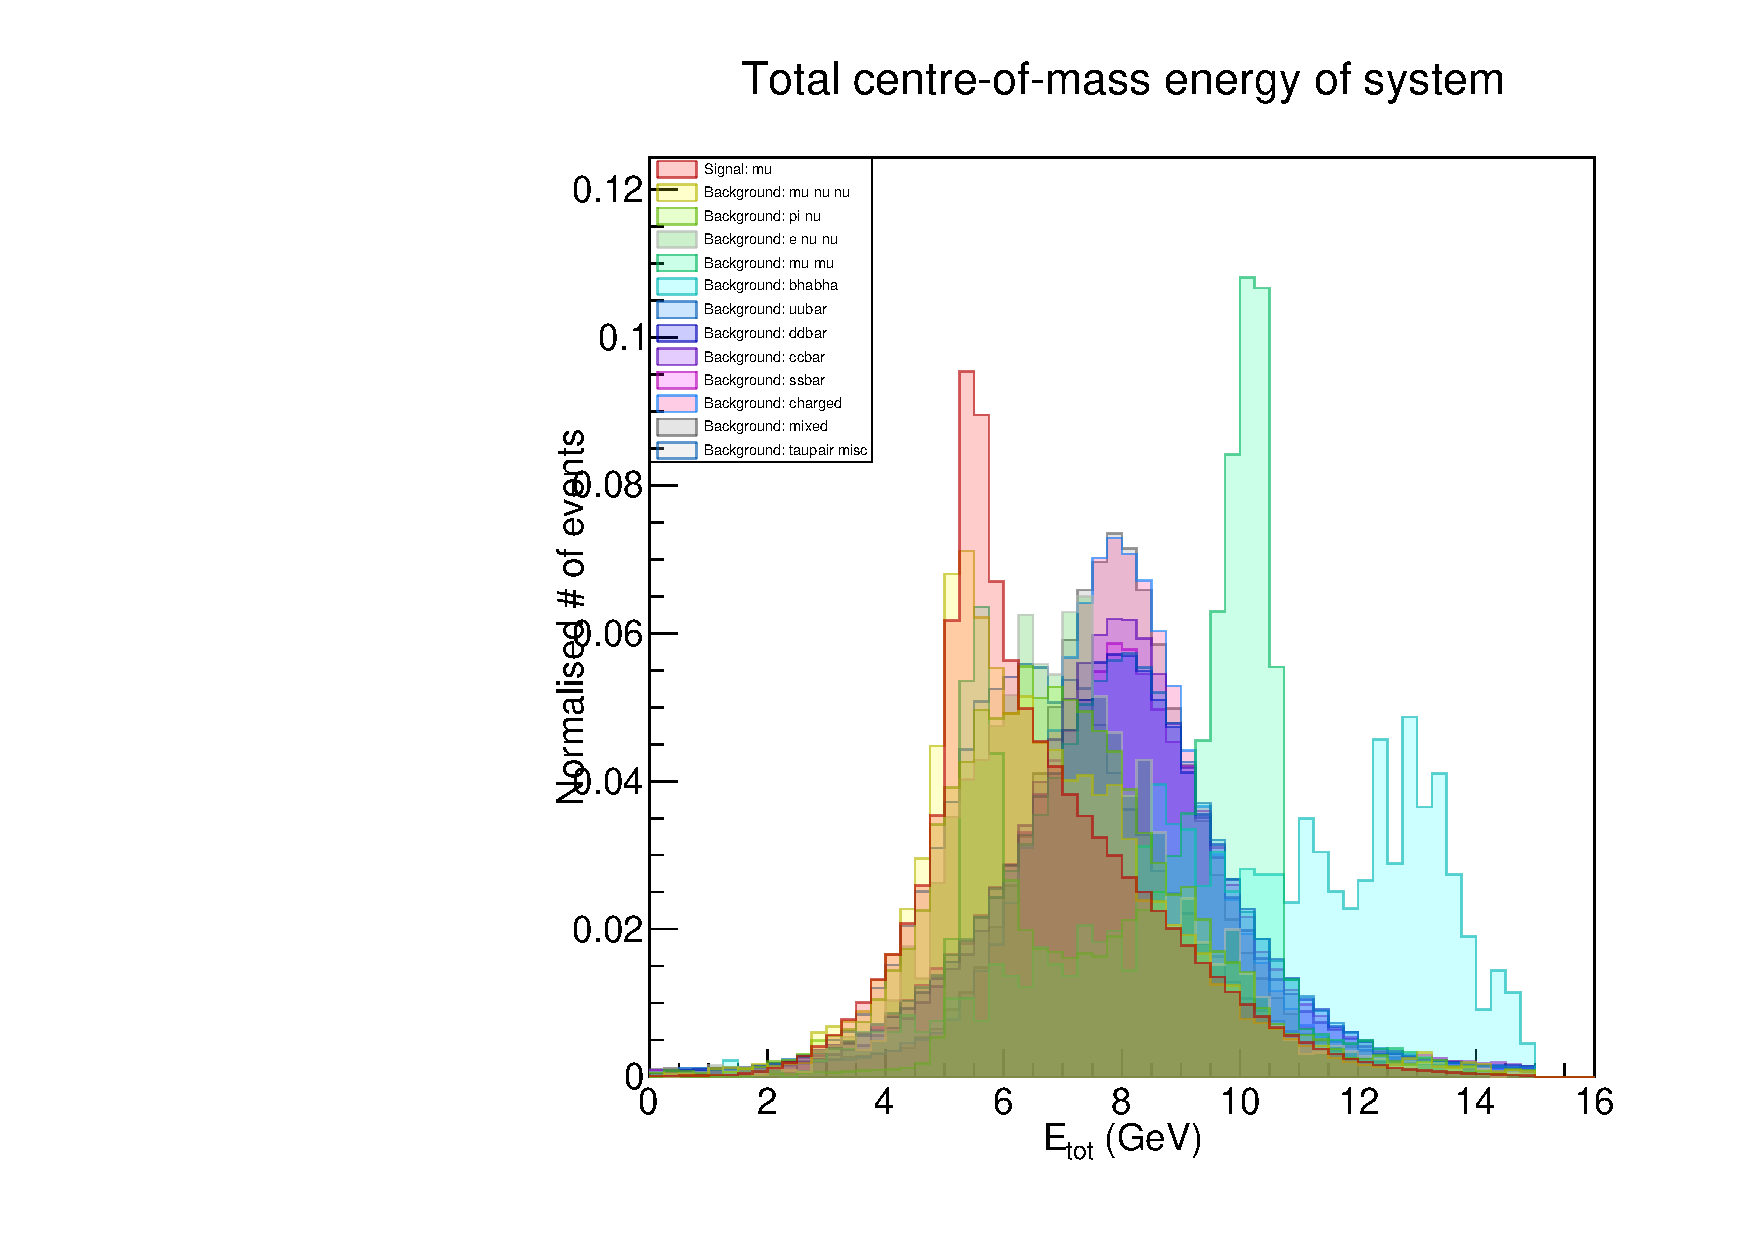
\includegraphics[width=\linewidth]{images/stack/stack_cut6_totalCM_E.pdf}
  \captionof{figure}{A figure}
  \label{fig:test1}
\end{minipage}%
\begin{minipage}{.5\textwidth}
  \centering
  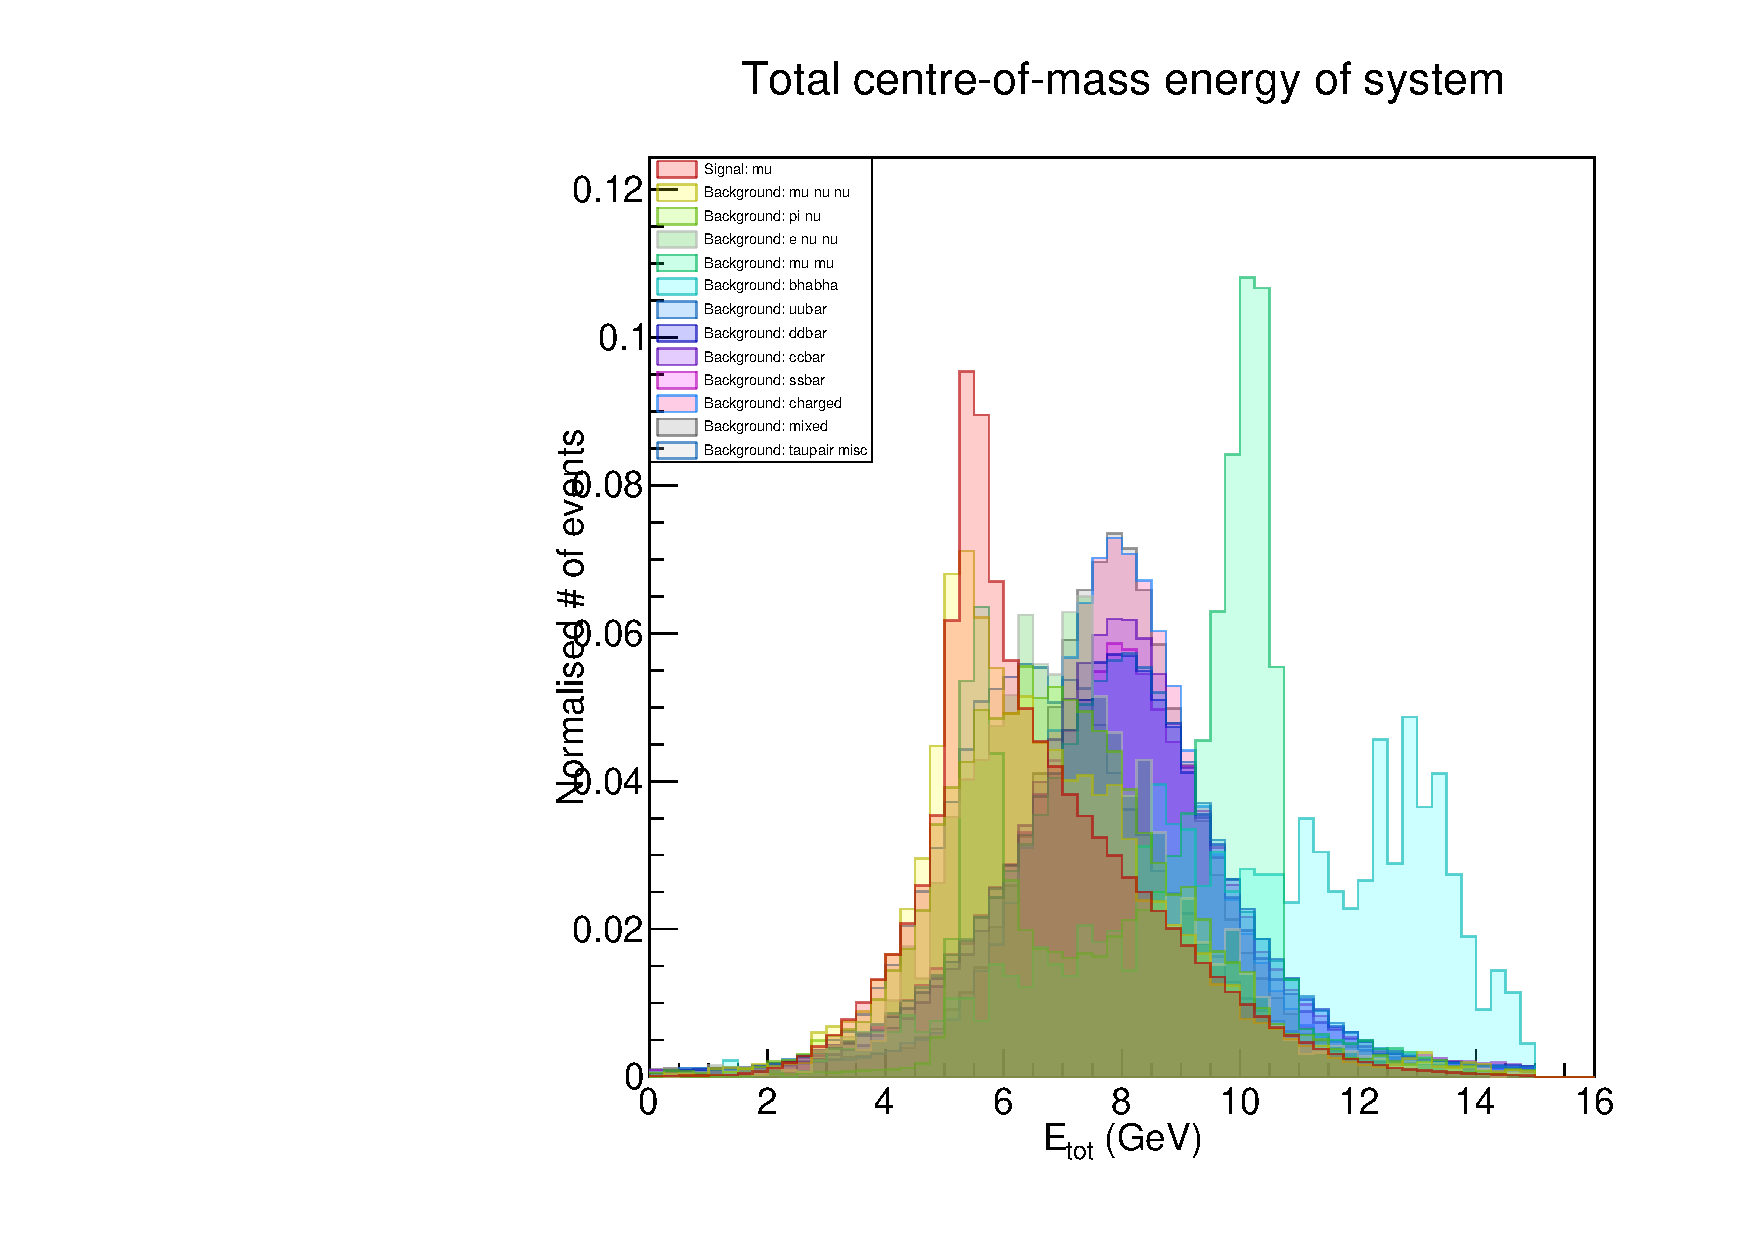
\includegraphics[width=\linewidth]{images/stack/stack_cut6_totalCM_E.pdf}
  \captionof{figure}{Another figure}
  \label{fig:test2}
\end{minipage}
\end{figure}

\begin{figure}[h]
\centering
\begin{minipage}{.5\textwidth}
  \centering
  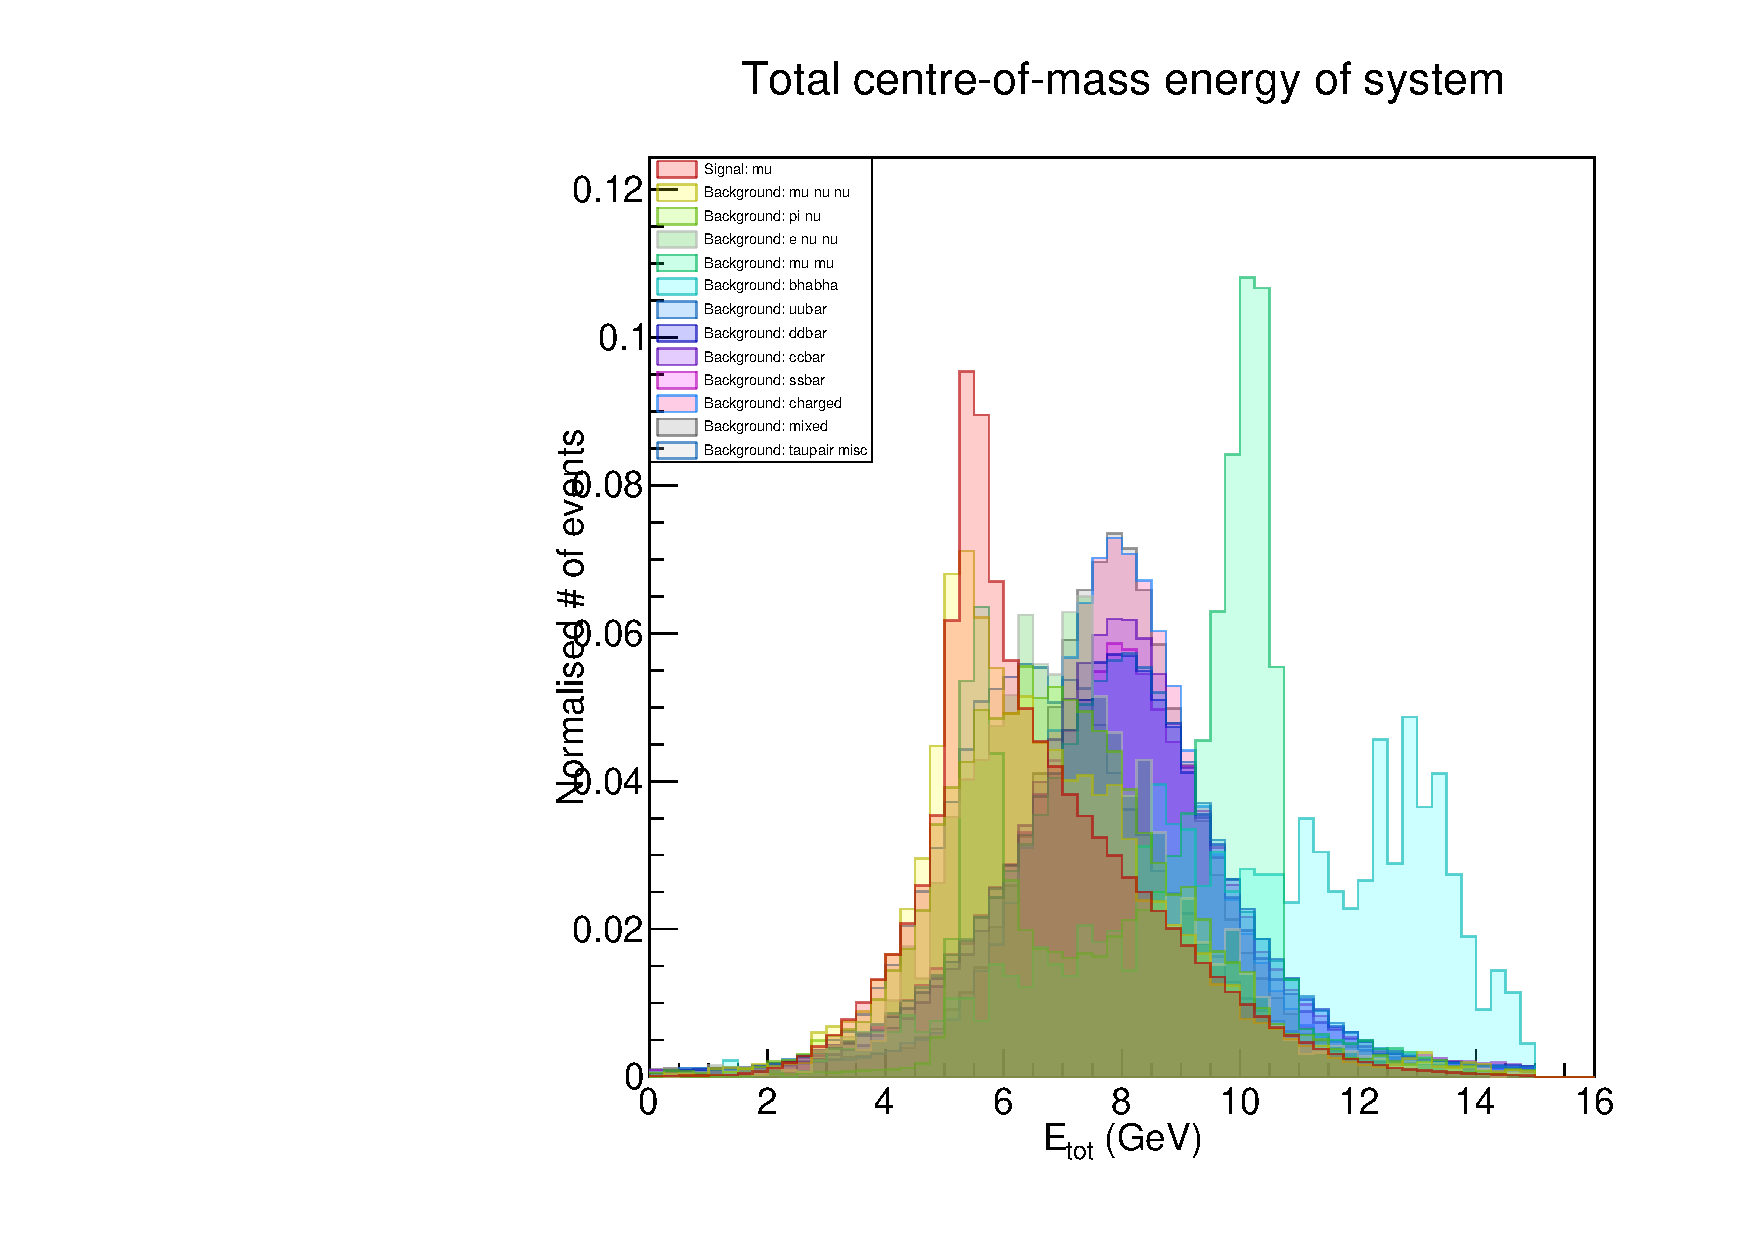
\includegraphics[width=\linewidth]{images/stack/stack_cut6_totalCM_E.pdf}
  \captionof{figure}{A figure}
  \label{fig:test1}
\end{minipage}%
\begin{minipage}{.5\textwidth}
  \centering
  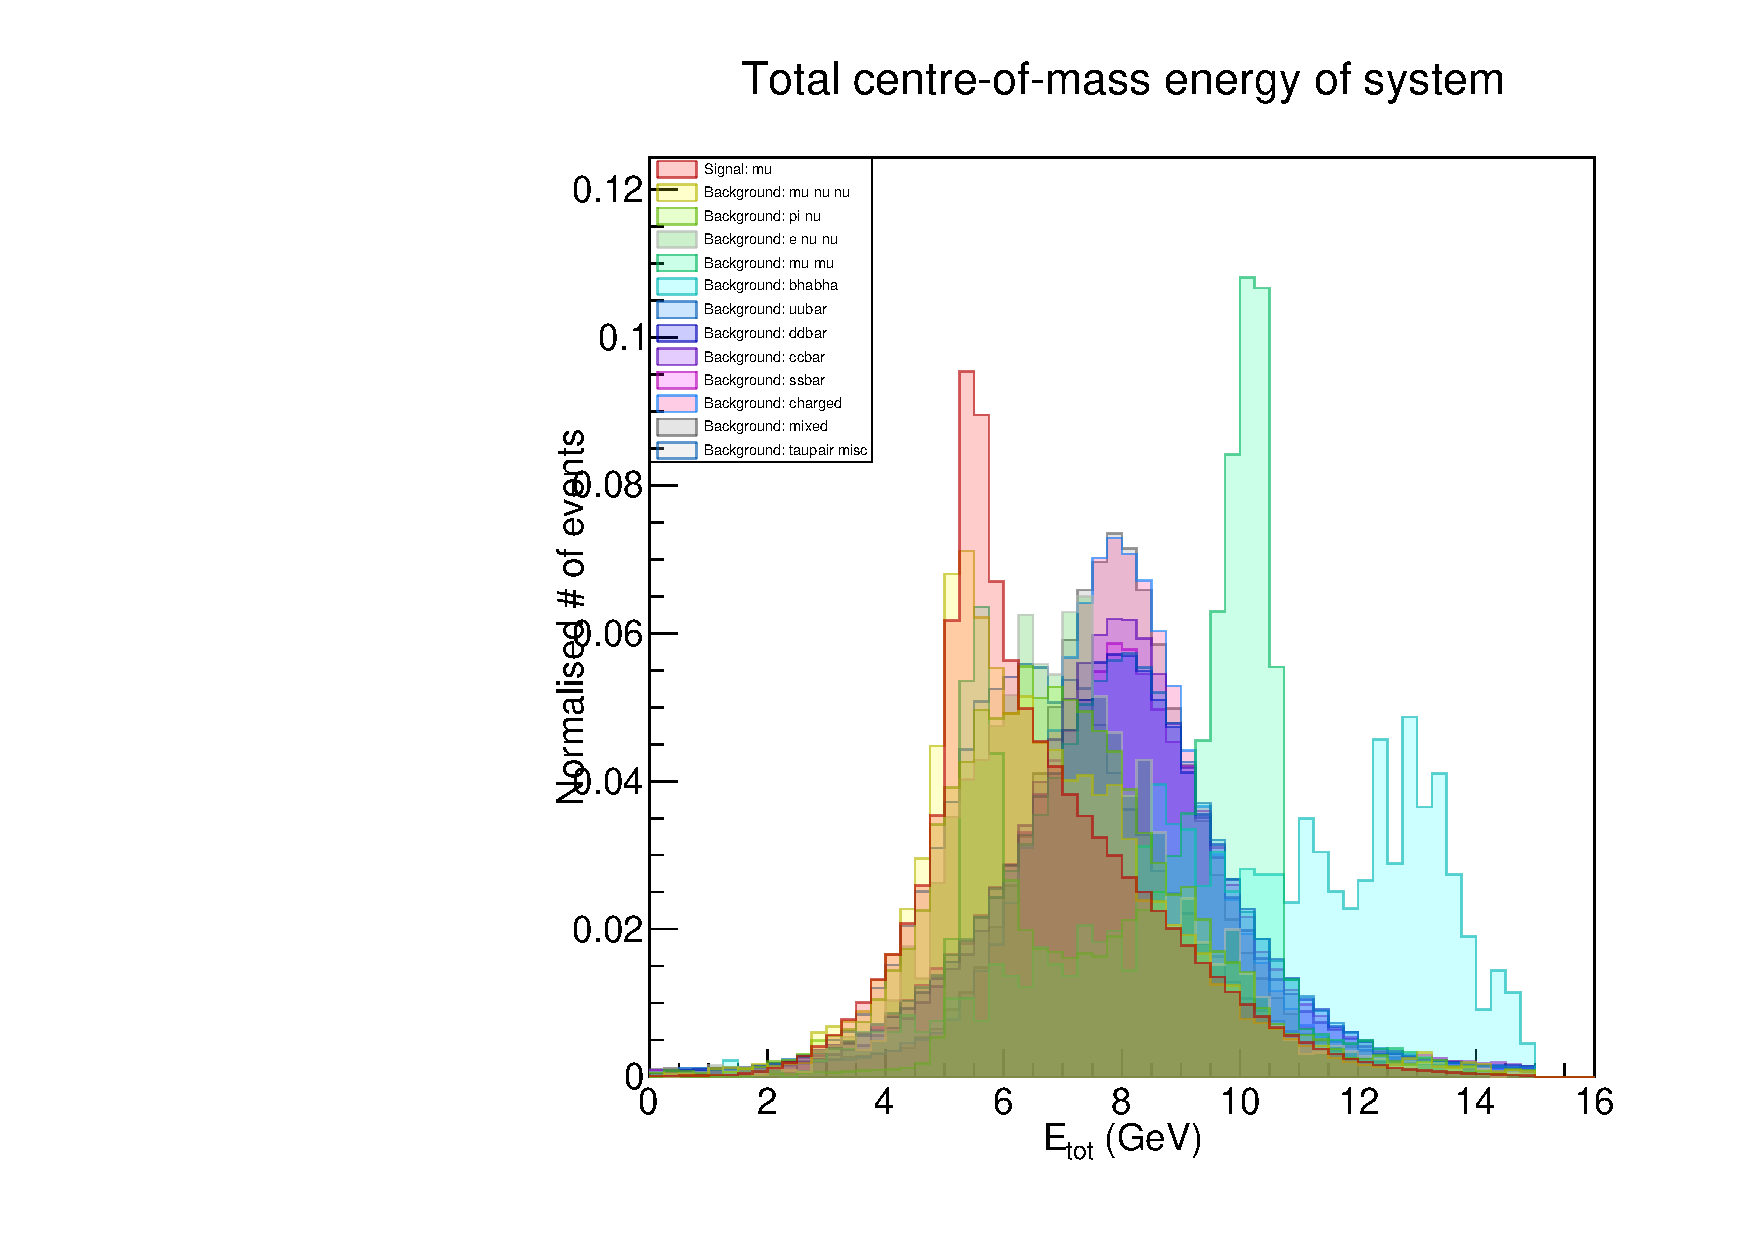
\includegraphics[width=\linewidth]{images/stack/stack_cut6_totalCM_E.pdf}
  \captionof{figure}{Another figure}
  \label{fig:test2}
\end{minipage}
\end{figure}

\subsection{Electron mode}

Much of the kinematics and topologies as described for the signal muon mode also applies to the signal electron mode. However, it is prudent to note the major difference between the two final state charged particles - specifically the difference in mass. Muons have mass $\SI{105.66}{MeV/c^2}$, over 200 times heavier than electrons, with mass of $\SI{0.511}{MeV/c^2}$. Due to their lighter mass, electrons lose far more energy due to bremsstrahlung (braking radiation), as given by

\begin{align}
P &= \text{radiated power} = \frac{e^2a^2 \gamma^4}{6},
\intertext{where}
e &= \text{electron charge},\\
a&= \text{particle acceleration},\\
\lambda &= \text{relativistic factor},\\
\end{align}
and we have of course taken particle physics units $c=\pi=\epsilon_0 = 1$. Since $E=\gamma mc^2$, radiated power from bremsstrahlung goes as $m^{-4}$; electrons lose more energy via bremsstrahlung than muons by factor $\left(m_{\mu}/m_{e}\right)^{4} \sim 200^4$.

This energy in the form of photons is deposited in the ECL clusters; a non-negligible amount of radiation from beam background is also deposited in these clusters, making accurate energy reconstruction of the signal electron difficult (??? is this right, or is it just that the electron has less energy? What is the ``energy/momentum'' variable.... E/P at creation?). Due to this energy loss we see a different energy and momentum 	signature for the signal track compared to the muon mode; peaks for both are located around XXXX GeV, but a large fraction of events have energies much lower.

Accurate reconstruction via \texttt{basf2} is more difficult for these lighter particles, with only a fraction of $\tau\to e\gamma$ events having a reconstructed $\tau$ invariant mass peak anywhere near the $\tau$ mass.


\begin{figure}[h]
\centering
\begin{minipage}{.5\textwidth}
  \centering
  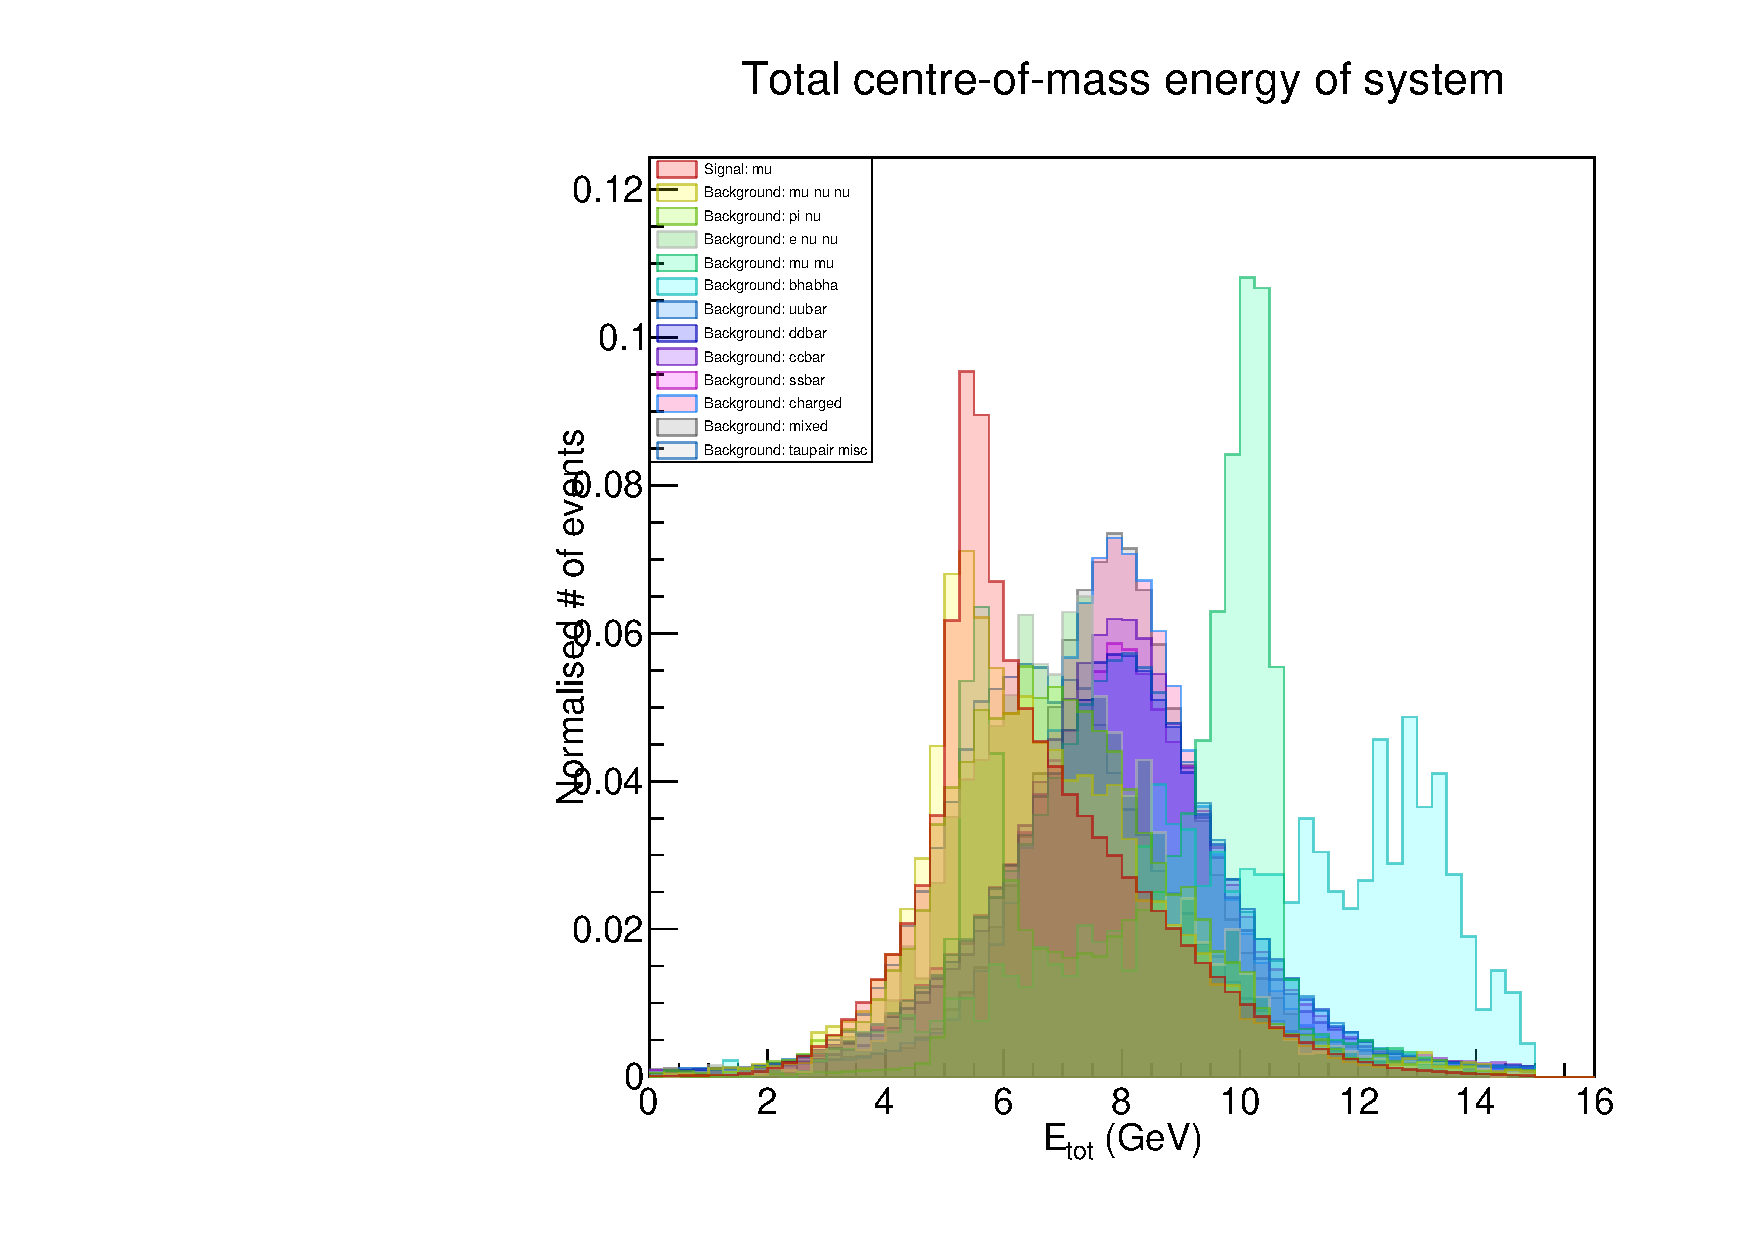
\includegraphics[width=\linewidth]{images/stack/stack_cut6_totalCM_E.pdf}
  \captionof{figure}{A figure}
  \label{fig:test1}
\end{minipage}%
\begin{minipage}{.5\textwidth}
  \centering
  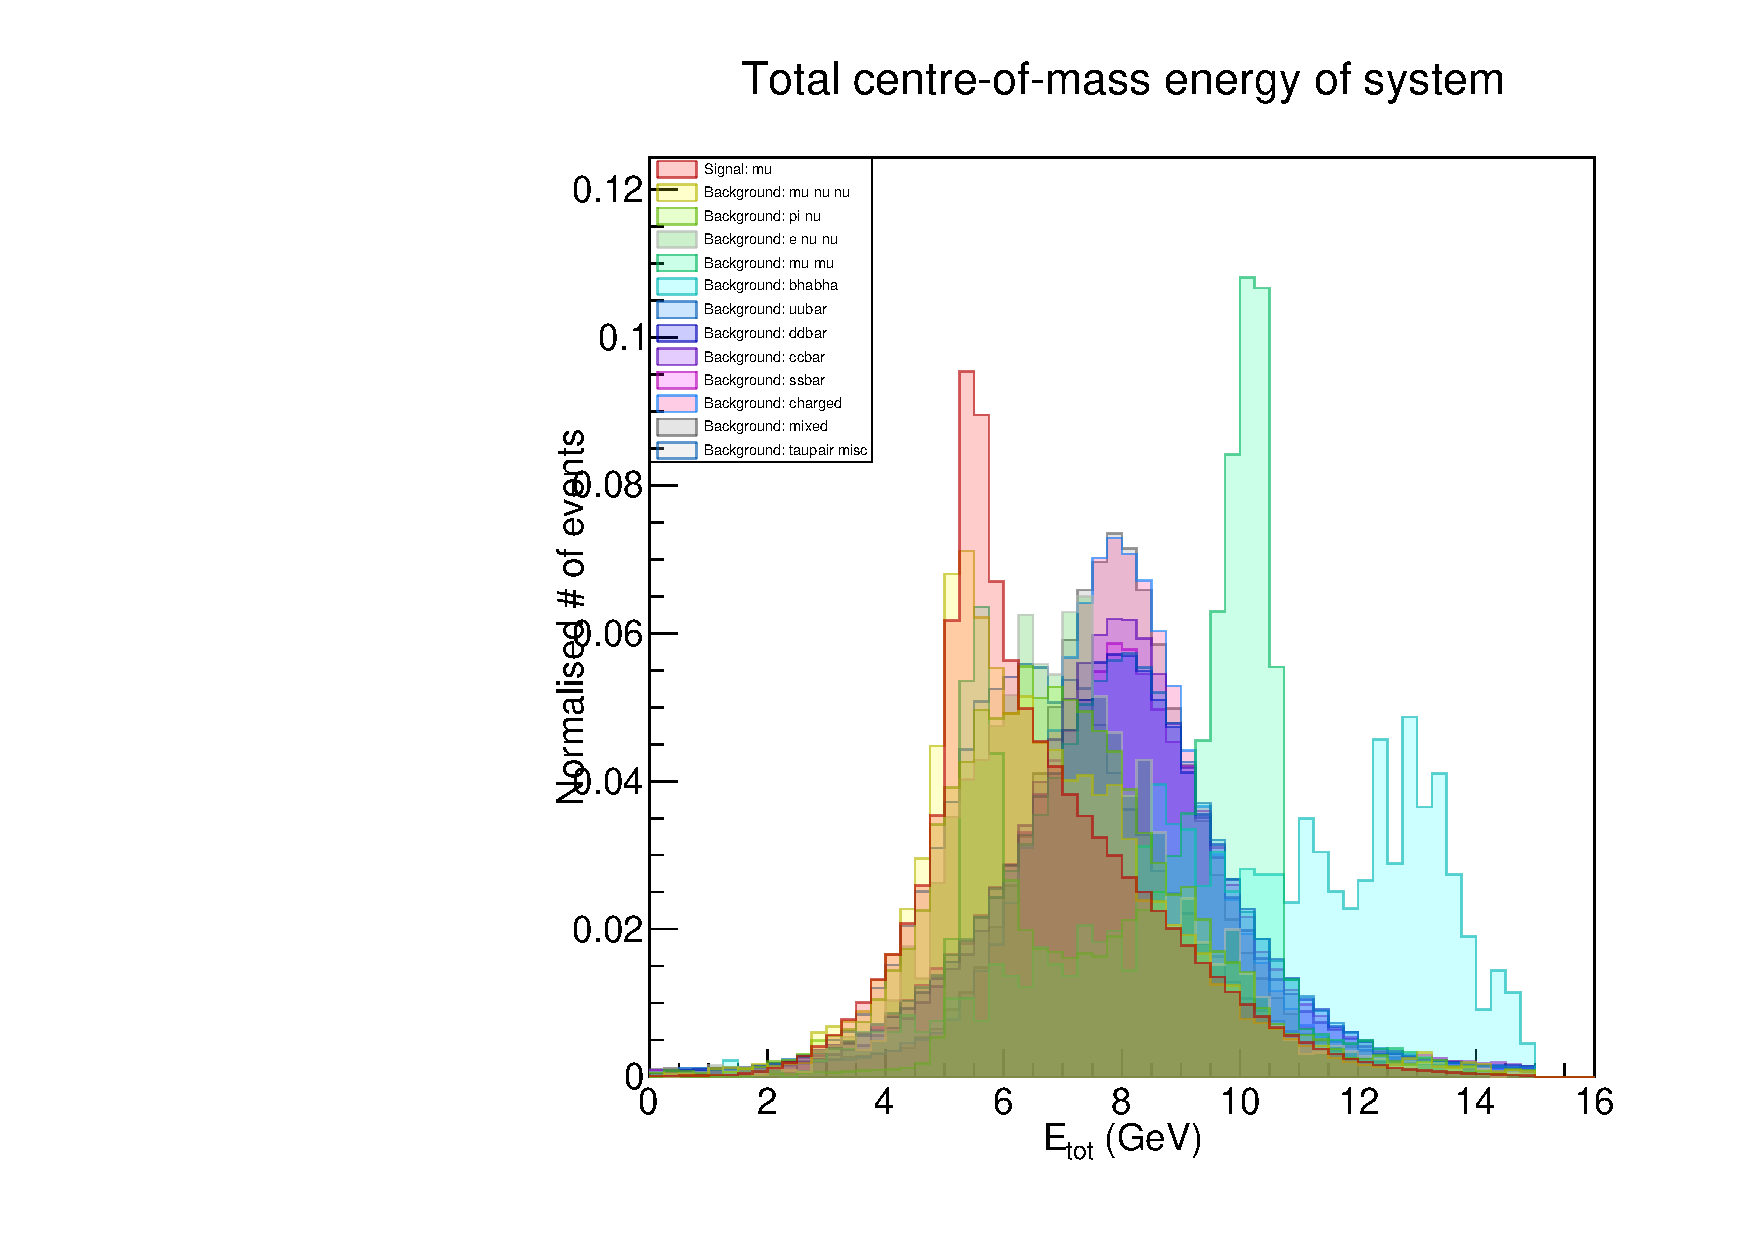
\includegraphics[width=\linewidth]{images/stack/stack_cut6_totalCM_E.pdf}
  \captionof{figure}{Another figure}
  \label{fig:test2}
\end{minipage}
\end{figure}

\begin{figure}[h]
\centering
\begin{minipage}{.5\textwidth}
  \centering
  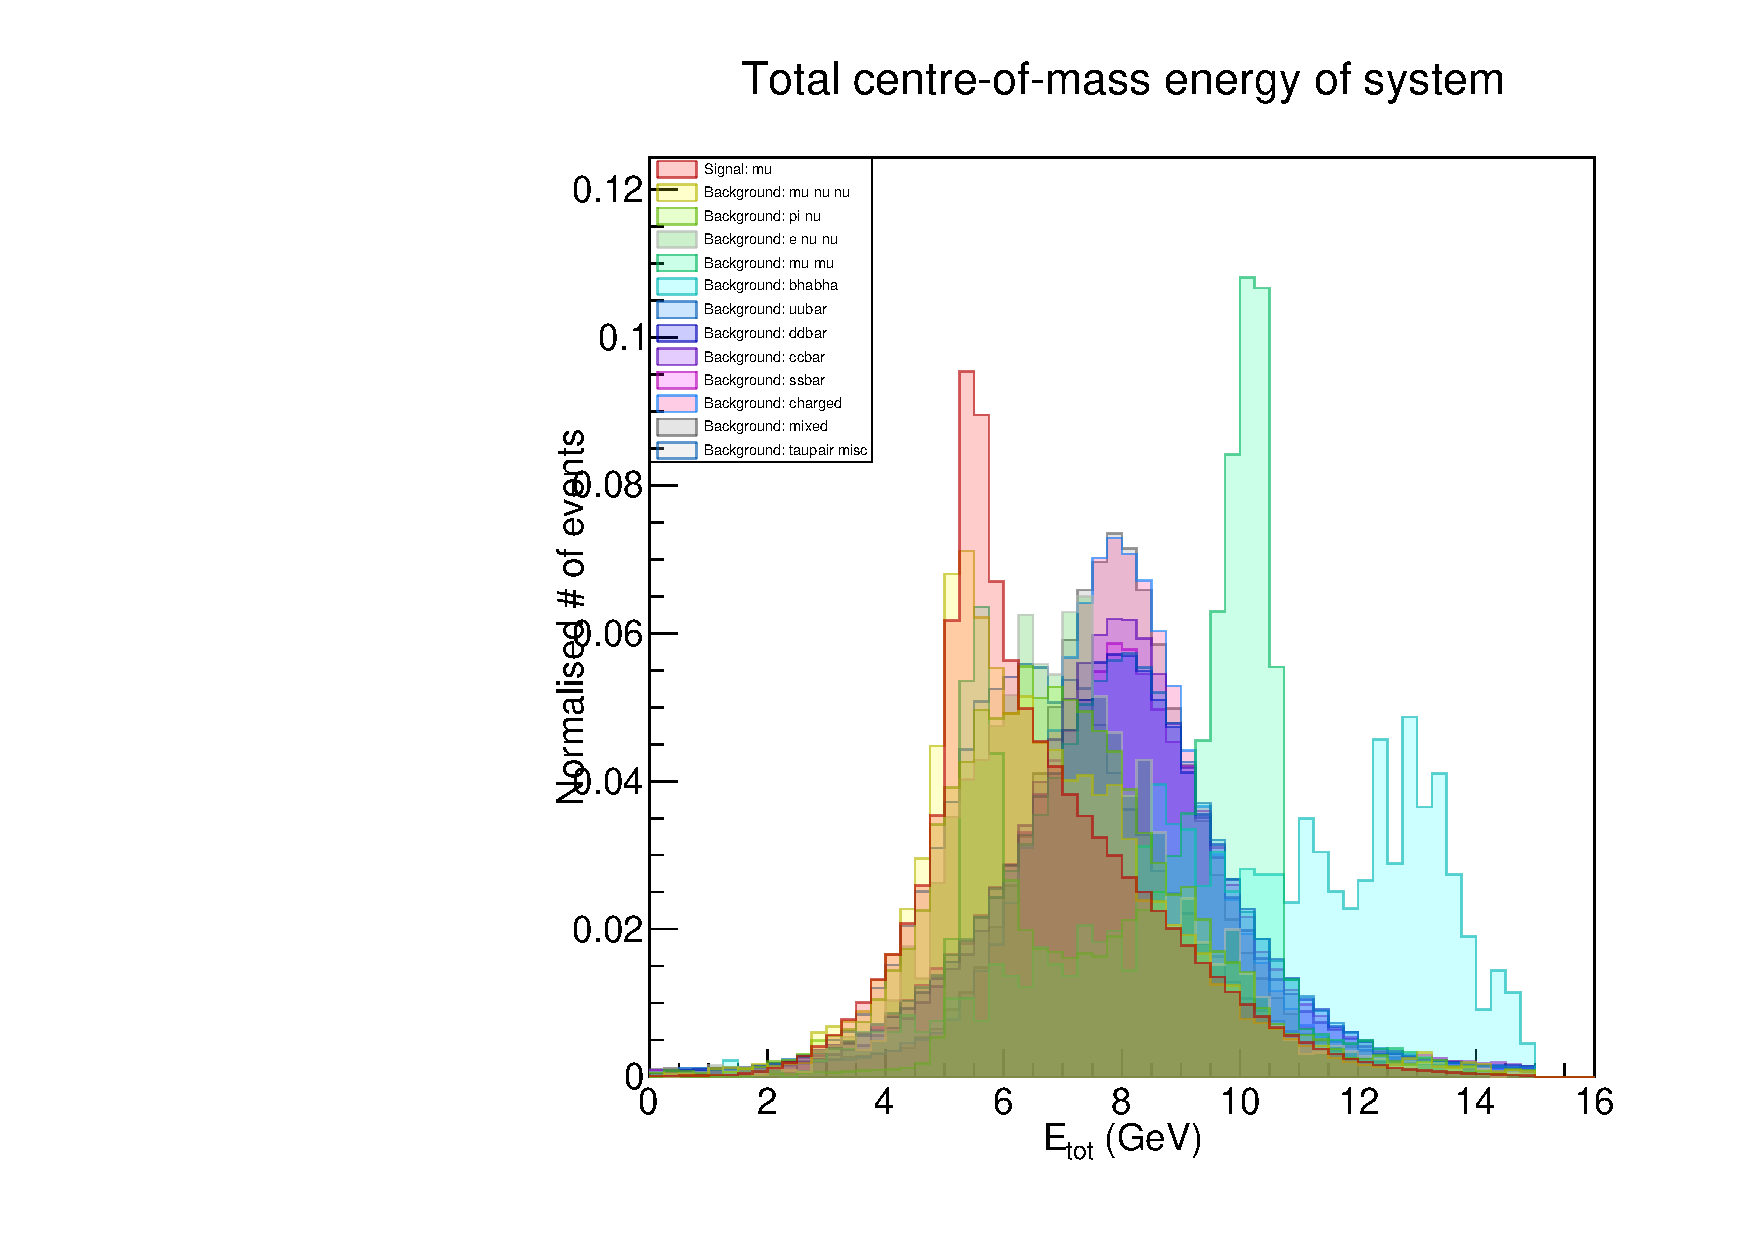
\includegraphics[width=\linewidth]{images/stack/stack_cut6_totalCM_E.pdf}
  \captionof{figure}{A figure}
  \label{fig:test1}
\end{minipage}%
\begin{minipage}{.5\textwidth}
  \centering
  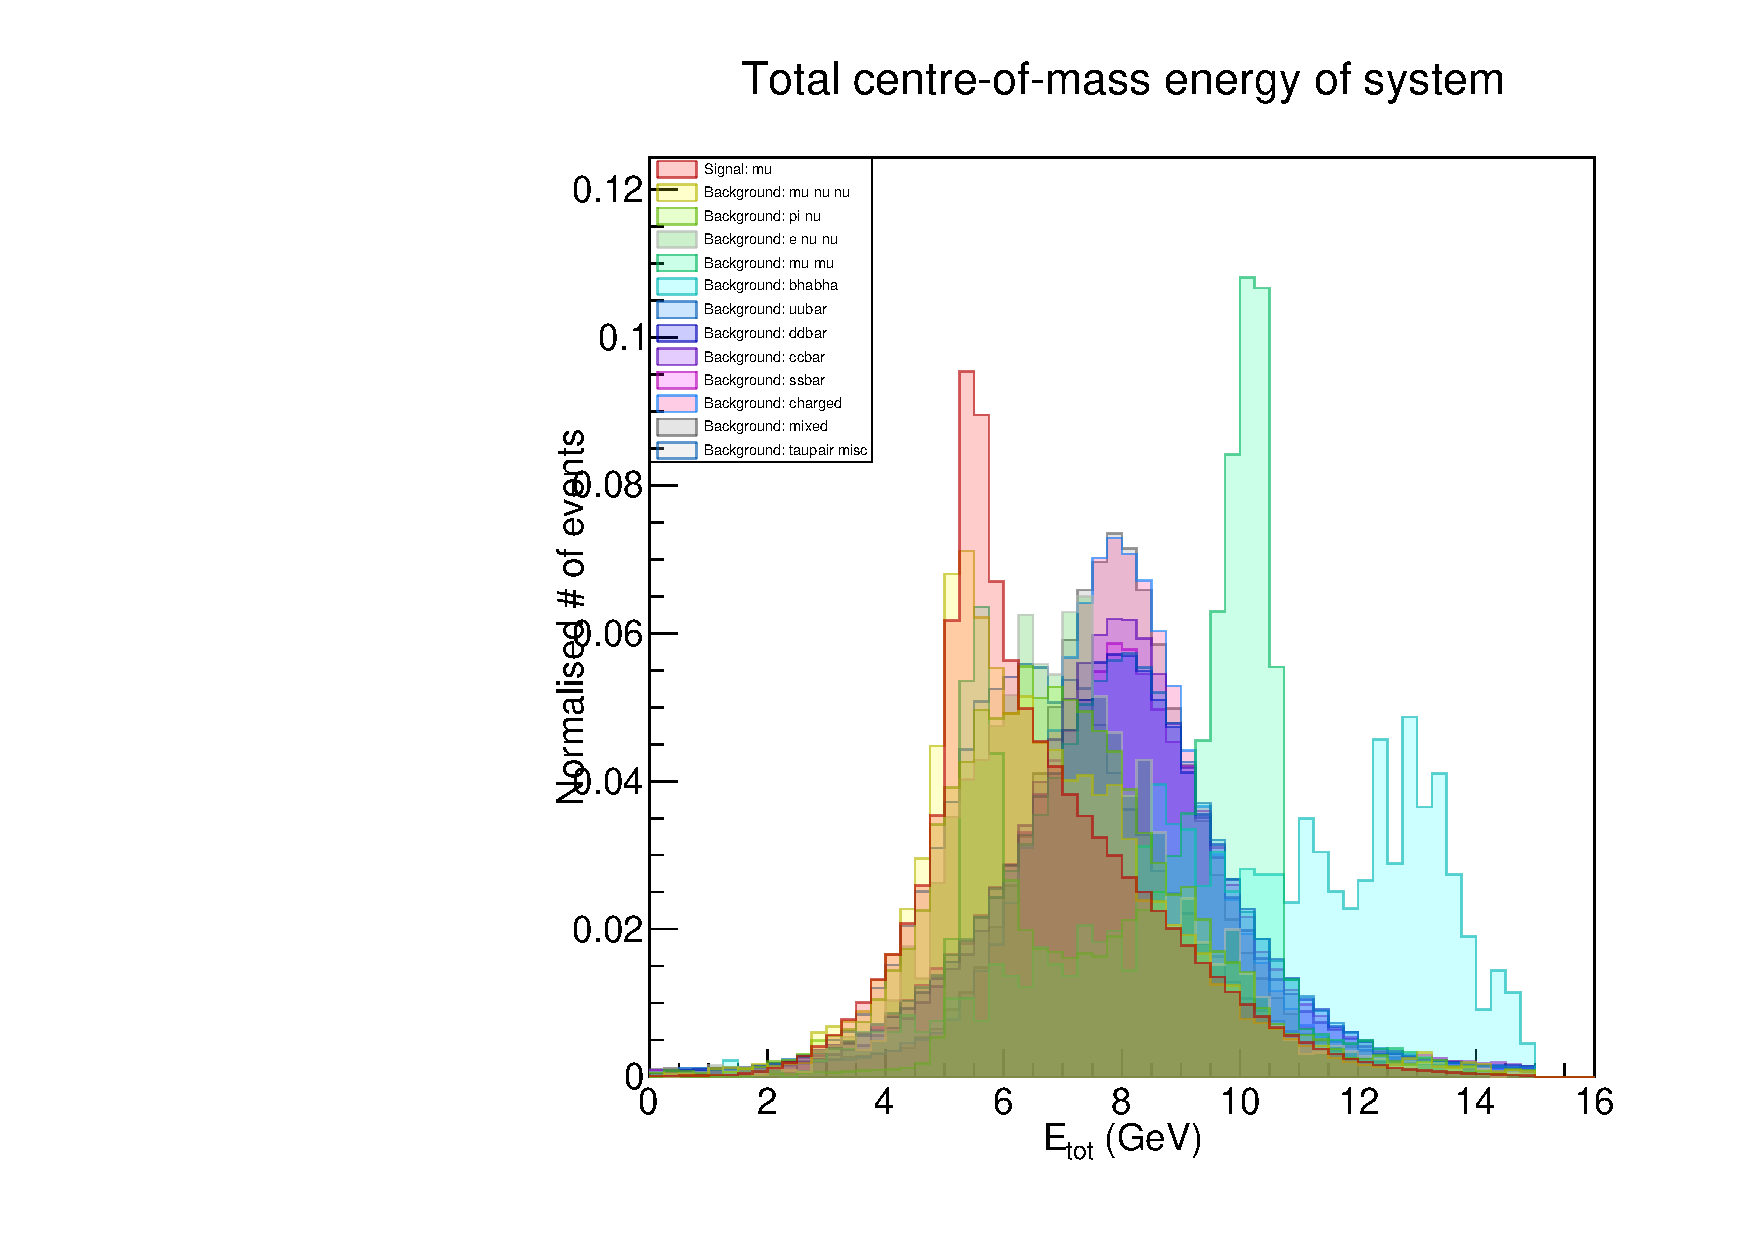
\includegraphics[width=\linewidth]{images/stack/stack_cut6_totalCM_E.pdf}
  \captionof{figure}{Another figure}
  \label{fig:test2}
\end{minipage}
\end{figure}


\pagebreak

\section{Backgrounds}

\subsection{Tau-pair processes}

A key difference between tau-pair backgrounds and the signal modes investigated is the lack of signal-side photon, and the existence of signal-side neutrinos.

We discuss the dominant tau-pair backgrounds $\tau\to e\nu\nu$, $\tau\to\mu\nu\nu$ and $\tau\to\pi\nu$ (where the pion is, of course, charged), with some minor discussion of the remaining modes. In tau-pair processes, the signal-side $\tau$ of energy $\SI{5.5}{GeV}$ decays dominantly into a single charged track and a neutrino (or neutrinos, in the pion modes). Light neutrinos carry away only a fraction of the energy from its mother particle; we expect the signal track to have a peak in energy of $\approx\SI{5.5}{GeV}$. However, the electron will lose a significant fraction of its energy due to bremsstrahlung as it passes through the detector and hence have a lower average energy. Signal track center-of-mass momentum is shown in Figure XXXXX below.

None of the dominant tau decay processes proceed with the final state photon; in most cases the reconstructed signal photon comes from initial state radiation (???? discuss this) or beam backgrounds. Photons produced as beam background are often low energy, especially compared to the average photon energy from signal processes of $\sim \SI{2.25}{GeV}$. Signal photon energy for tau-pair processes is shown in Figure XXXX; we note the peak energy of of $<\SI{1}{GeV}$. 

Since the signal photon does not originate from the signal-side $\tau$, the signal tracks appears ``boosted'' by comparison. This ``boost'' leads to the signal track and signal photon travelling almost back-to-back in the center-of-mass frame, in contrast to the signal mode where these final state particles have only a small opening angle between them.  


Since the signal track originates from the signal-side $\tau$ and is hence boosted in the center-of-mass frame by its mother particle,

Since this signal photon does not originate from the signal-side $\tau$, but instead from beam background or occasionally the tag-side $\tau$.

SOMETHING ABOUT E9E25.


\begin{figure}[h]
\centering
\begin{minipage}{.5\textwidth}
  \centering
  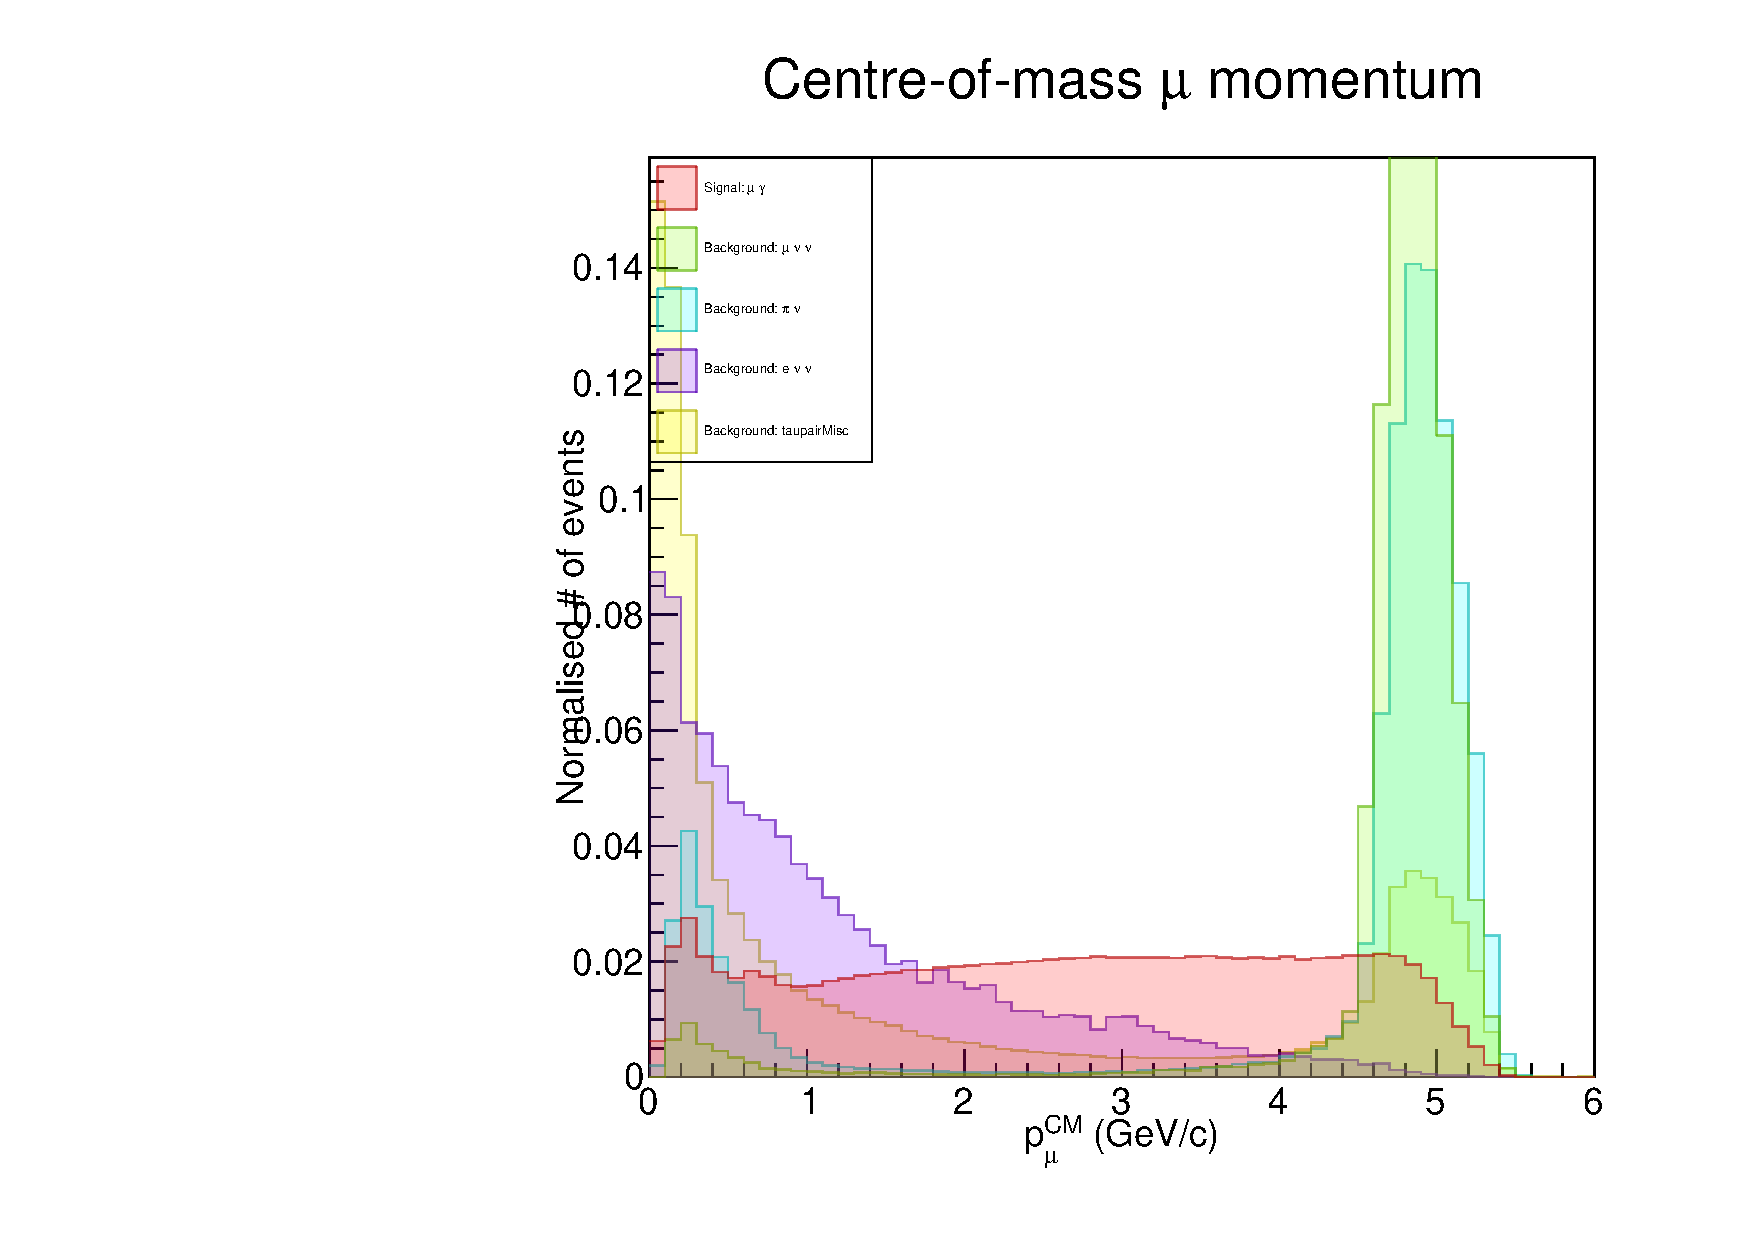
\includegraphics[width=\linewidth]{images/taupair-muCM_P.pdf}
  \captionof{figure}{Taupair - muCM P}
  \label{fig:test1}
\end{minipage}%
\begin{minipage}{.5\textwidth}
  \centering
  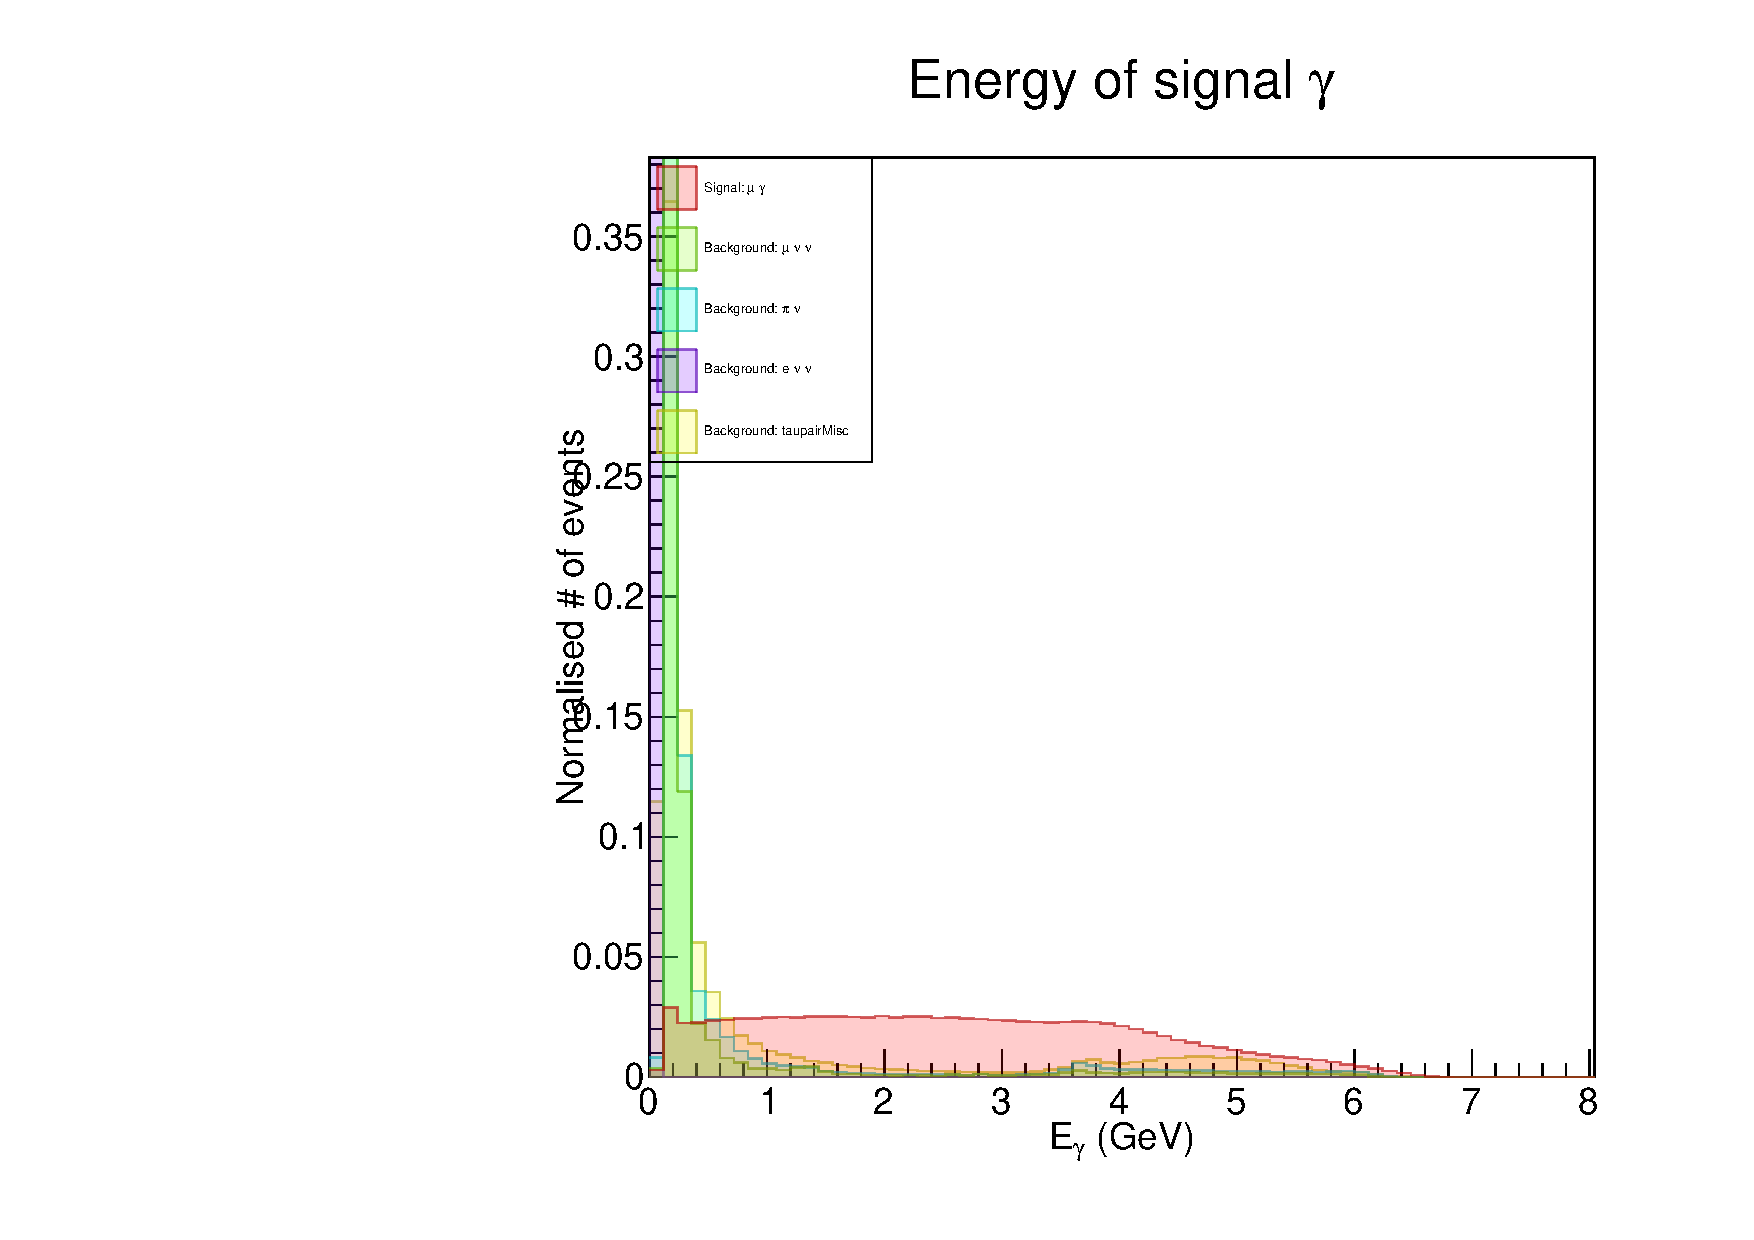
\includegraphics[width=\linewidth]{images/taupair-gamma_E.pdf}
  \captionof{figure}{Taupair - gamma E}
  \label{fig:test2}
\end{minipage}
\end{figure}

\begin{figure}[h]
\centering
\begin{minipage}{.5\textwidth}
  \centering
  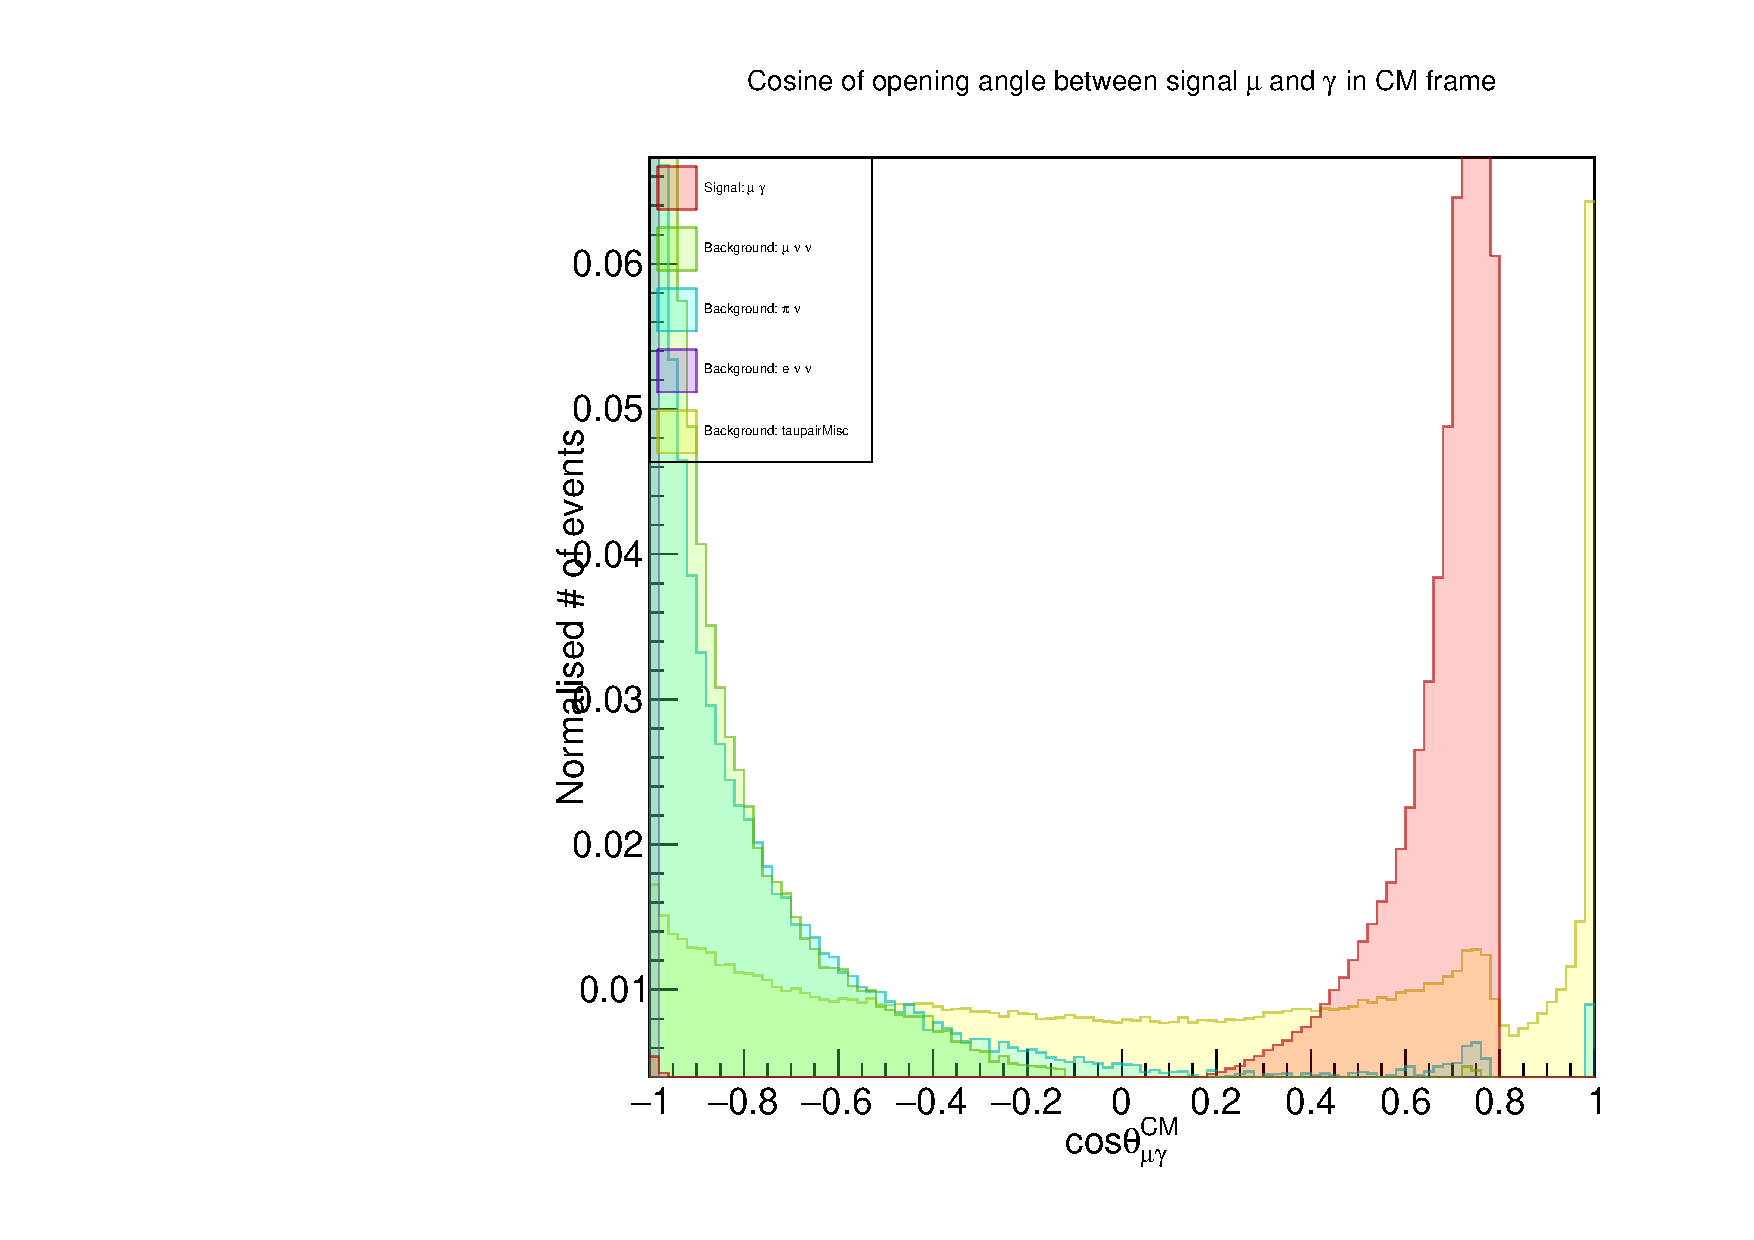
\includegraphics[width=\linewidth]{images/taupair-muGammaOpeningCM.pdf}
  \captionof{figure}{Taupair - muGammaOpeningCosThetaCM}
  \label{fig:test1}
\end{minipage}%
\begin{minipage}{.5\textwidth}
  \centering
  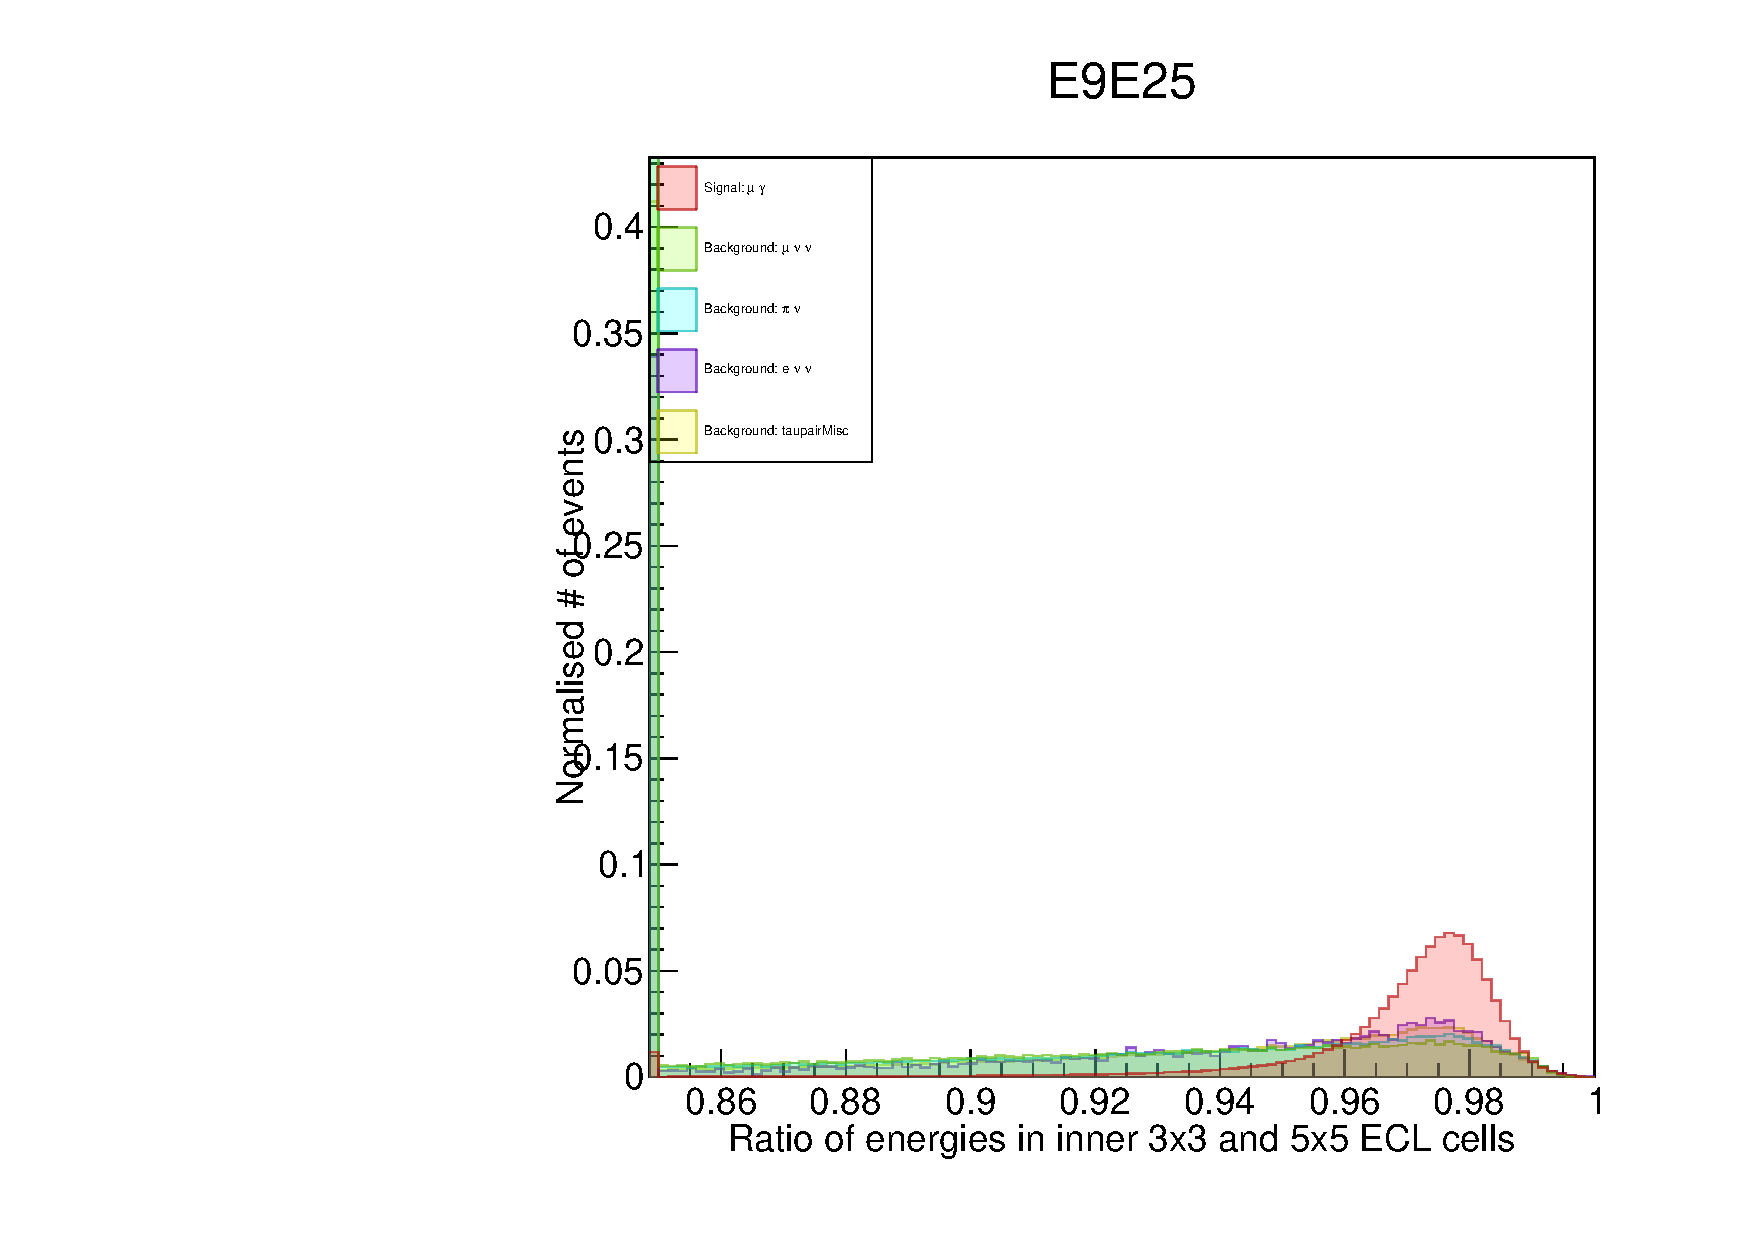
\includegraphics[width=\linewidth]{images/taupair-e9e25.pdf}
  \captionof{figure}{Taupair -E9E25}
  \label{fig:test2}
\end{minipage}
\end{figure}


\subsection{Mu-pair processes}

Muons are very cleanly reconstructed by the detector; they do not lose any significant amount of energy through bremsstrahlung radiation, and they penetrate deeply leaving a distinct signal. Unlike the tau-pair processes or the signal modes discussed above, mu-pair processes $e^+ e^- \to \mu^+ \mu^- (\gamma)$, both signal- and tag-side channels consist of only a single charged track each, sometimes with a final state photon. Hence, mu-pair processes are reconstructed very well. This is evidenced by the majority of events with only two reconstructed tracks (see Figure XXXX); this is is stark comparison to the spread of tracks from two up to fifteen in tau-pair events. Total reconstructed energy peaks around $\SI{10.5}{GeV}$.

By momentum conservation, the signal and tag tracks are generated back-to-back for $\mu\mu$ final states (XXX \% of all mu-pair processes), or with an opening angle similar to the signal mode for $\mu\mu\gamma$ final states (XXXX \% of all mu-pair processes). The signal photon is often reconstructed from low energy beam background photons, as with background tau-pair processes. A similar photon energy spectrum can be seen in Figure XXXX.

MORE TOPOLOGY STUFF?

\begin{figure}[h]
\centering
\begin{minipage}{.5\textwidth}
  \centering
  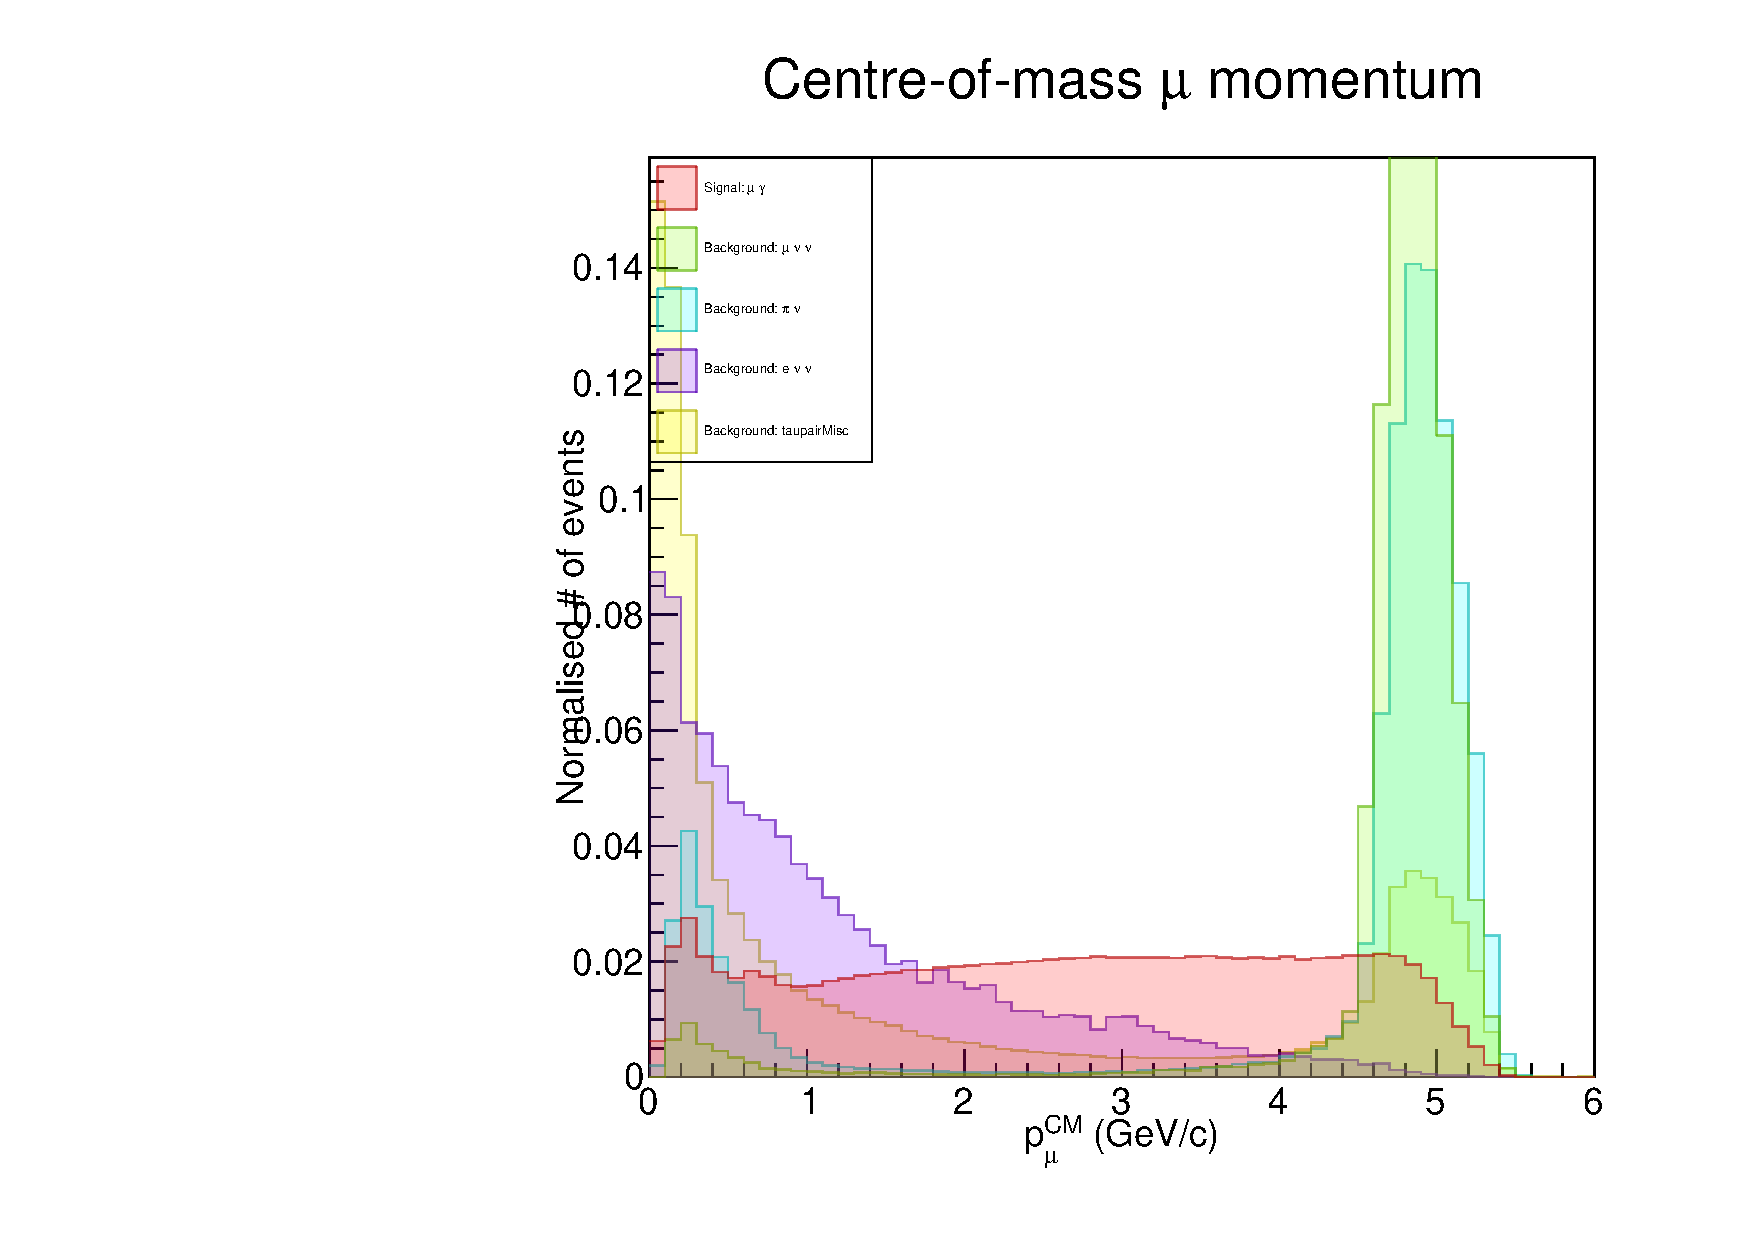
\includegraphics[width=\linewidth]{images/taupair-muCM_P.pdf}
  \captionof{figure}{Taupair - muCM P}
  \label{fig:test1}
\end{minipage}%
\begin{minipage}{.5\textwidth}
  \centering
  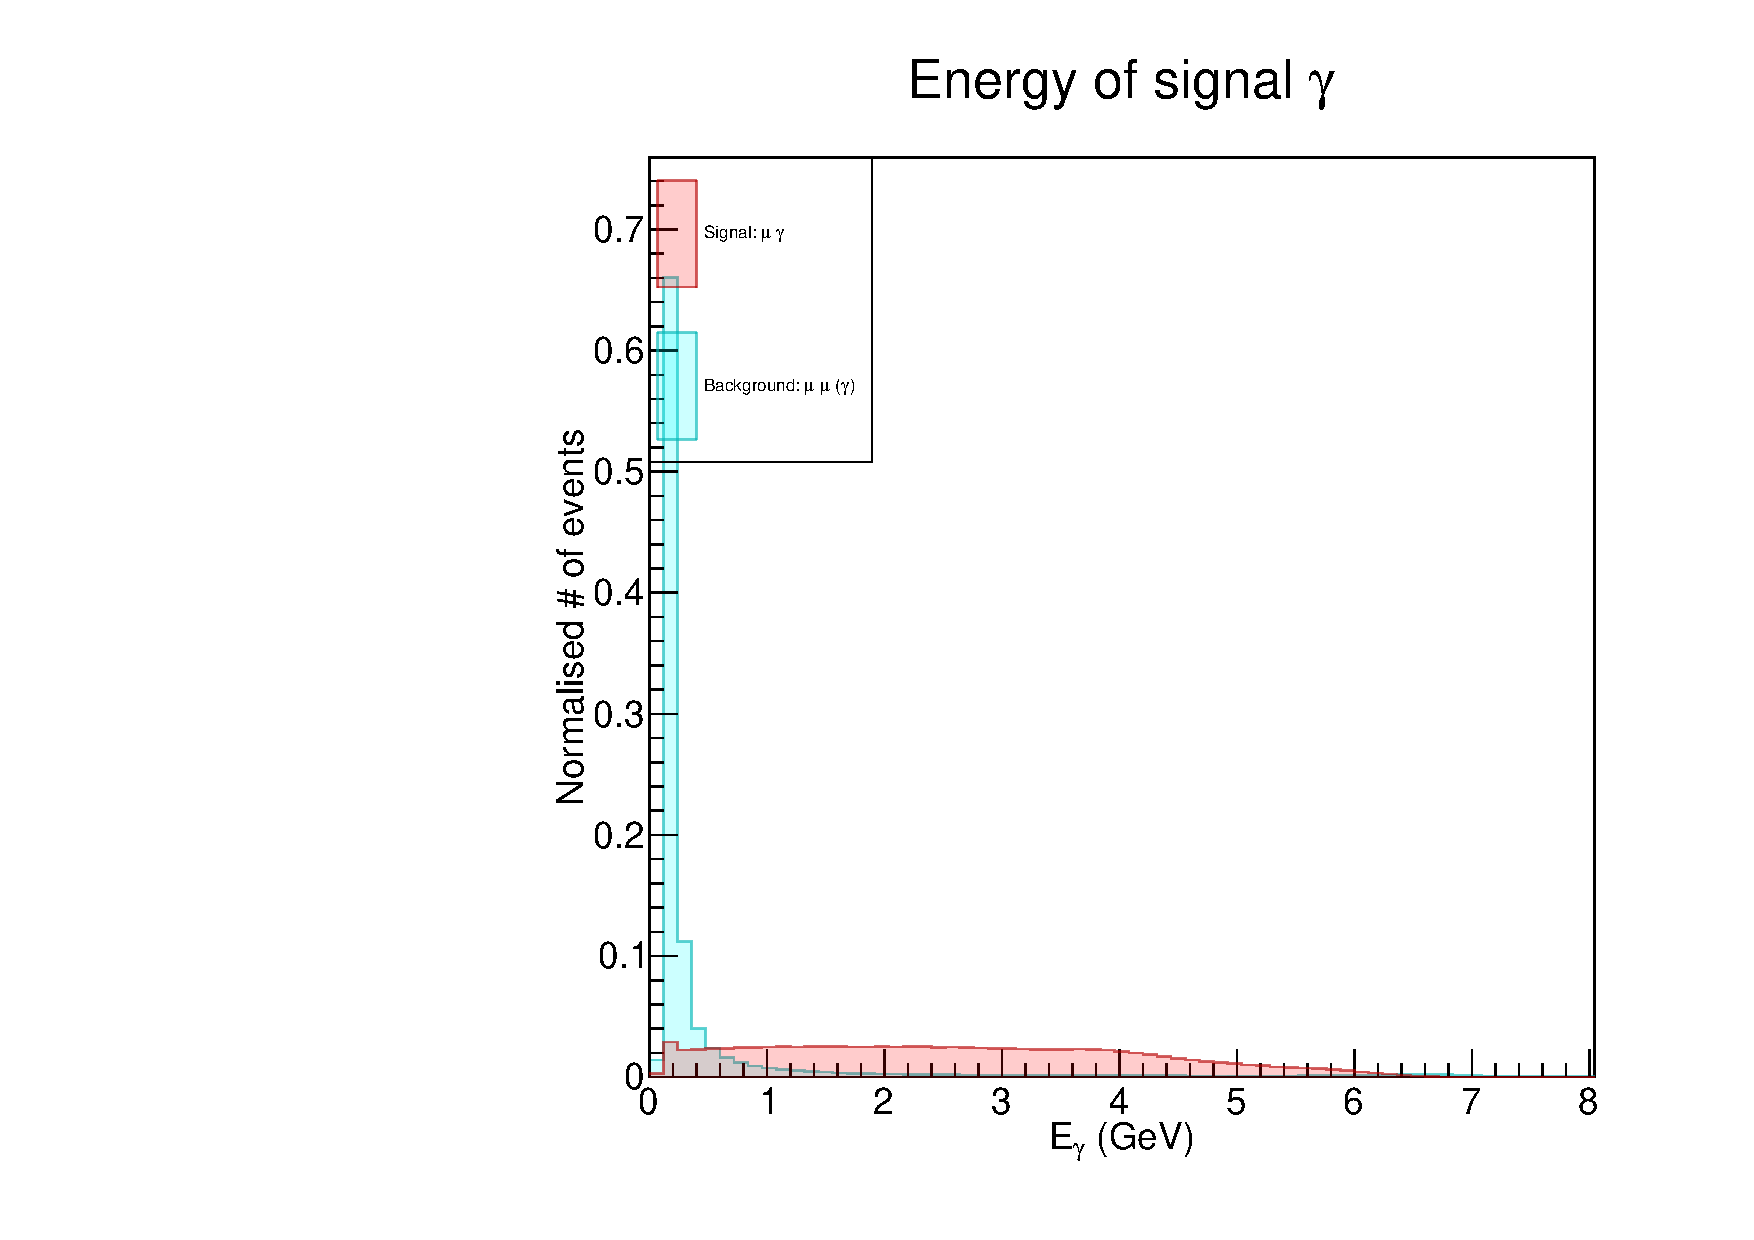
\includegraphics[width=\linewidth]{images/mupair-gamma_E.pdf}
  \captionof{figure}{Mu-pair: gamma E}
  \label{fig:test2}
\end{minipage}
\end{figure}

\begin{figure}[h]
\centering
\begin{minipage}{.5\textwidth}
  \centering
  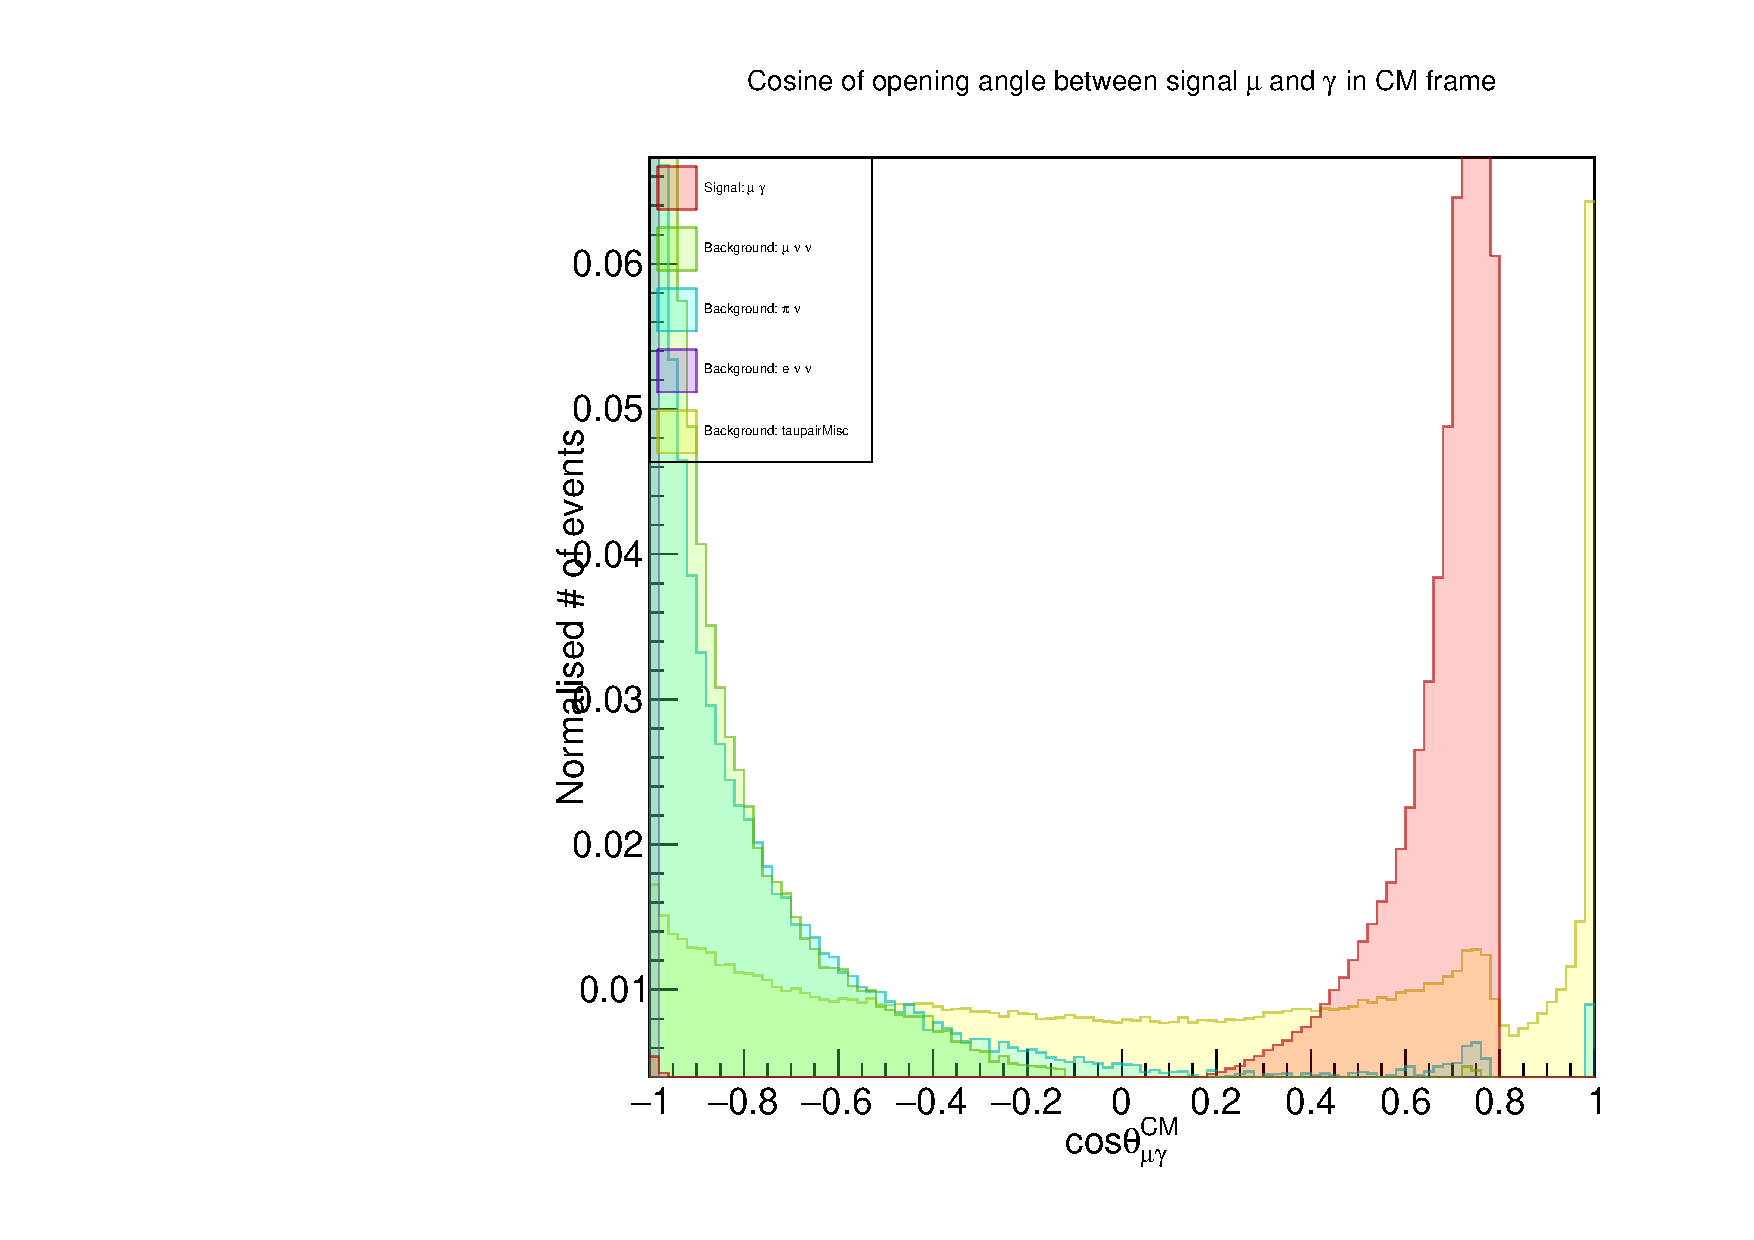
\includegraphics[width=\linewidth]{images/taupair-muGammaOpeningCM.pdf}
  \captionof{figure}{Taupair - muGammaOpeningCosThetaCM}
  \label{fig:test1}
\end{minipage}%
\begin{minipage}{.5\textwidth}
  \centering
  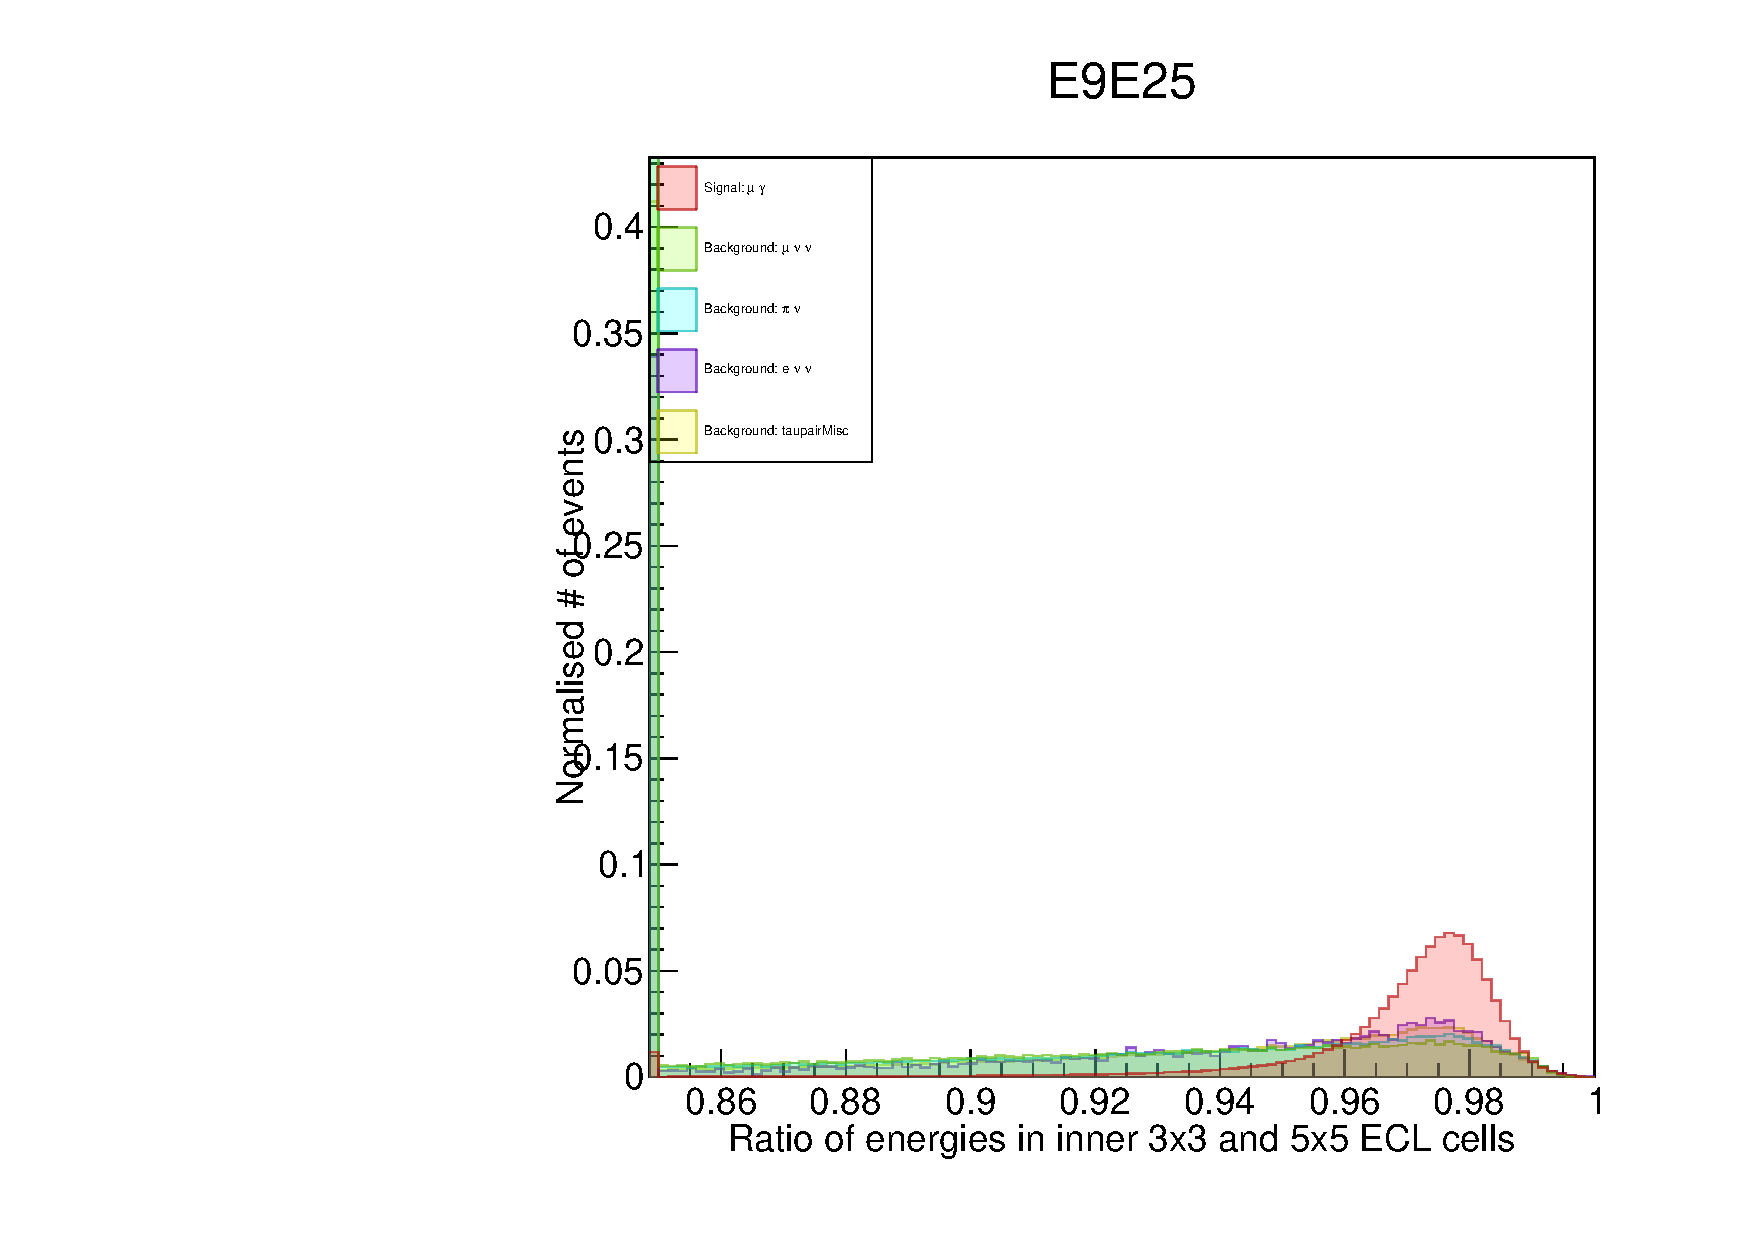
\includegraphics[width=\linewidth]{images/taupair-e9e25.pdf}
  \captionof{figure}{Taupair -E9E25}
  \label{fig:test2}
\end{minipage}
\end{figure}



\subsection{Bhabha}

Bhabha events $e^+ e^- \to e^+ e^- (\gamma)$ have event signatures (???) very similar to mu-pair processes $e^+ e^- \to \mu^+ \mu^- (\gamma)$, for obvious reasons. However, as is case with electrons in the detector, both signal and tag track particles lose a significant portion of their energy to bremsstrahlung and are not reconstructed as cleanly as muons. 

Smearing of energies and momenta occurs for bhabha event reconstruction, with measureables not peaking as strongly as for mu-pair events and instead spreading across a values. These features are shown in Figures XXX and XXX below, comparing distributions for mu-pair events to bhabha events. Much of the event topology is still common between these processes, however.

\begin{figure}[h]
\centering
\begin{minipage}{.5\textwidth}
  \centering
  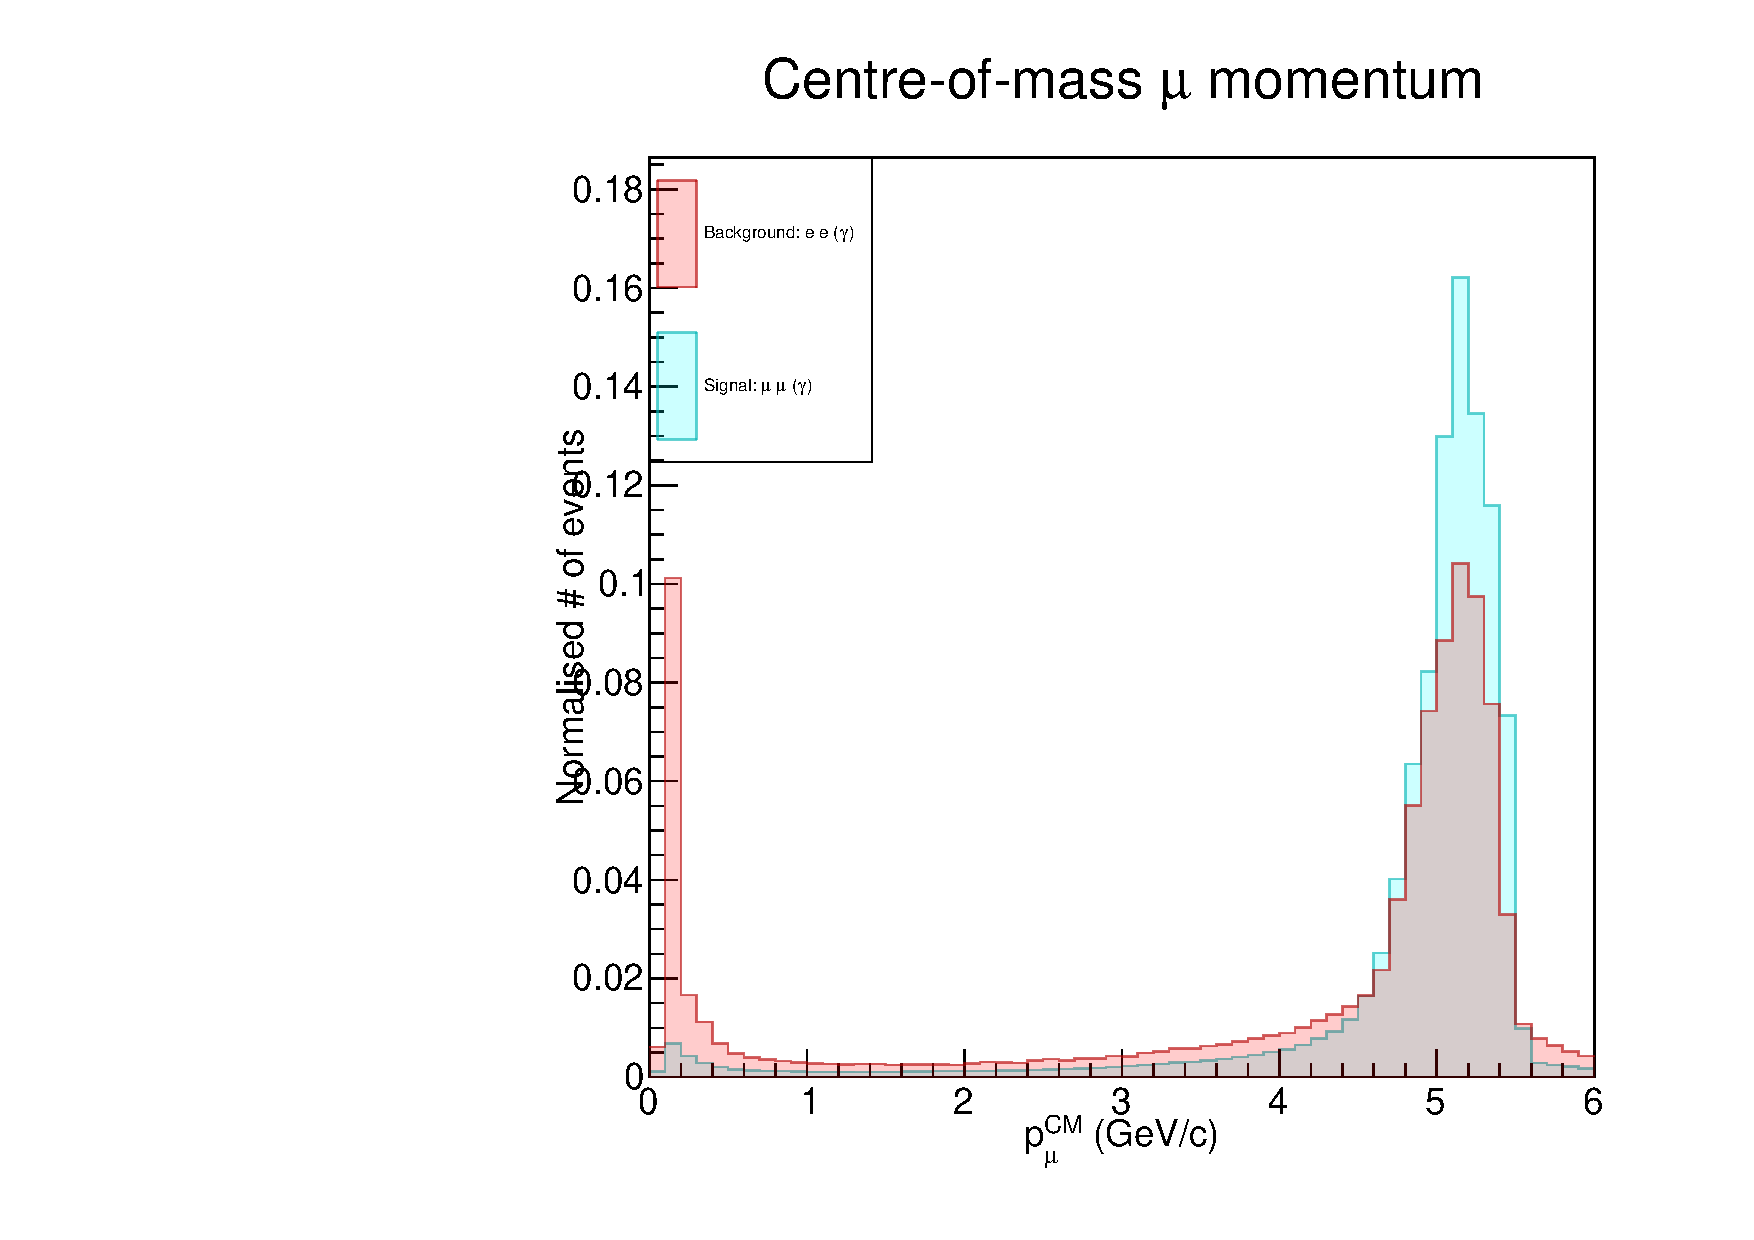
\includegraphics[width=\linewidth]{images/bhabha-mupair-muCM_P.pdf}
  \captionof{figure}{Bhabha: muCM P}
  \label{fig:test1}
\end{minipage}%
\begin{minipage}{.5\textwidth}
  \centering
  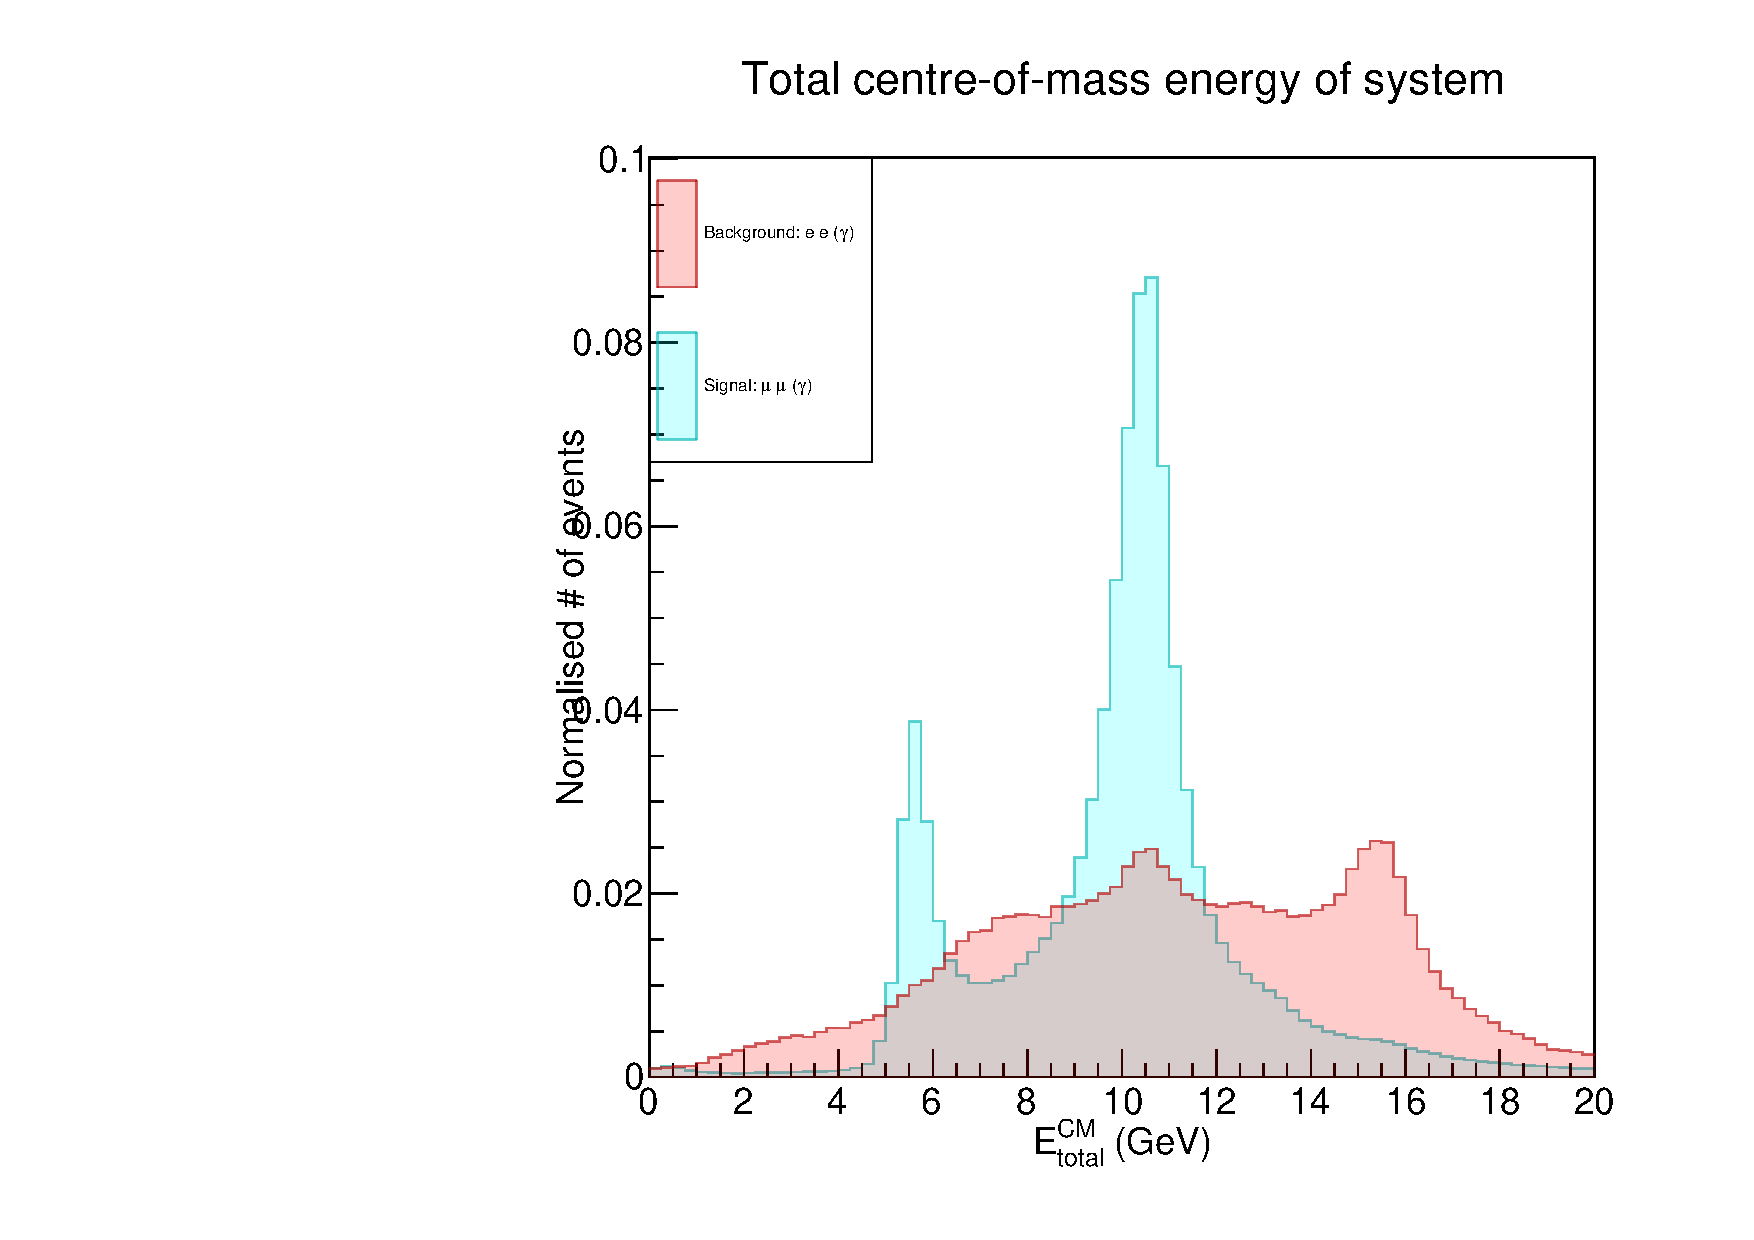
\includegraphics[width=\linewidth]{images/bhabha-mupair-totalCM_E.pdf}
  \captionof{figure}{Bhabha: totalCM E}
  \label{fig:test2}
\end{minipage}
\end{figure}


\subsection{Continuum and $B\bar{B}$}

NOT SURE HOW TO DESCRIBE TOPOLOGIES FOR THESE EVENTS


\begin{figure}[h]
\centering
\begin{minipage}{.5\textwidth}
  \centering
  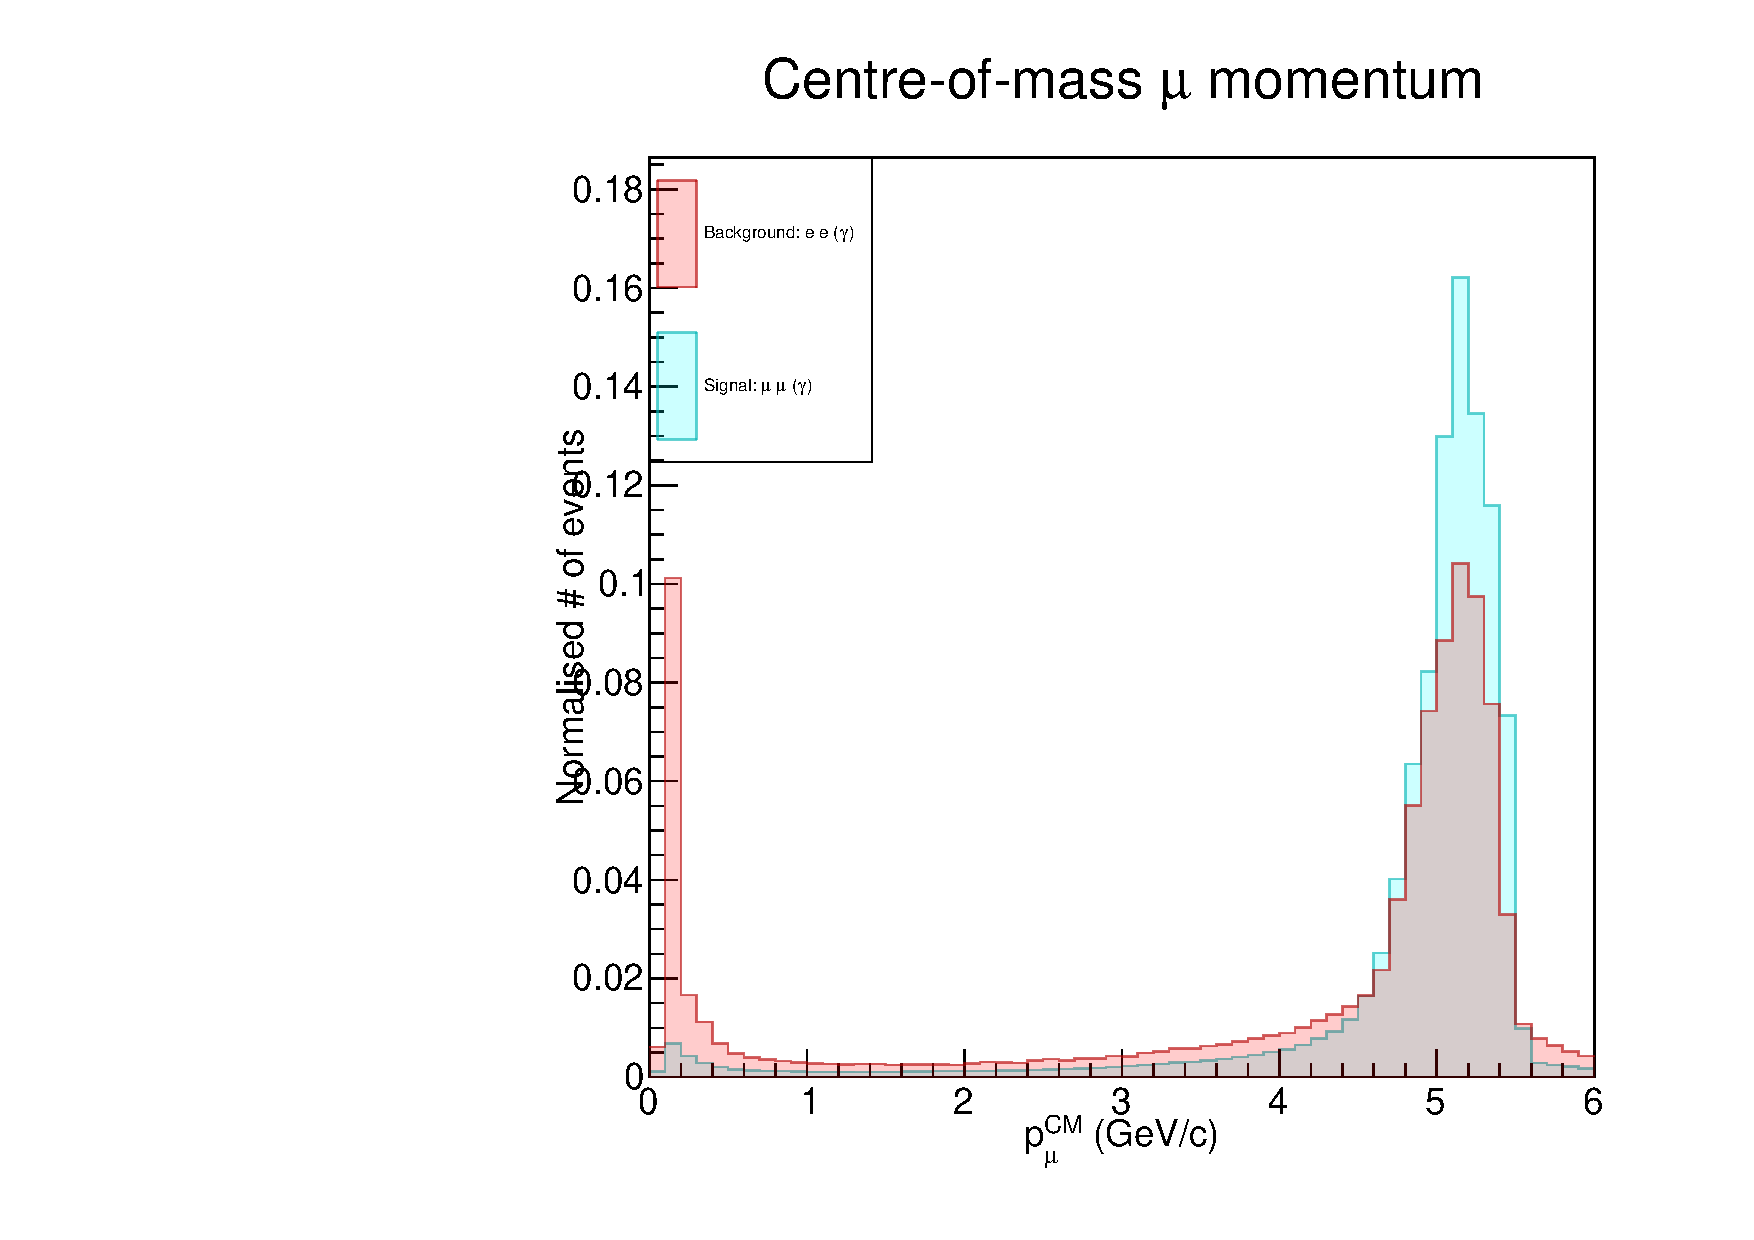
\includegraphics[width=\linewidth]{images/bhabha-mupair-muCM_P.pdf}
  \captionof{figure}{Bhabha: muCM P}
  \label{fig:test1}
\end{minipage}%
\begin{minipage}{.5\textwidth}
  \centering
  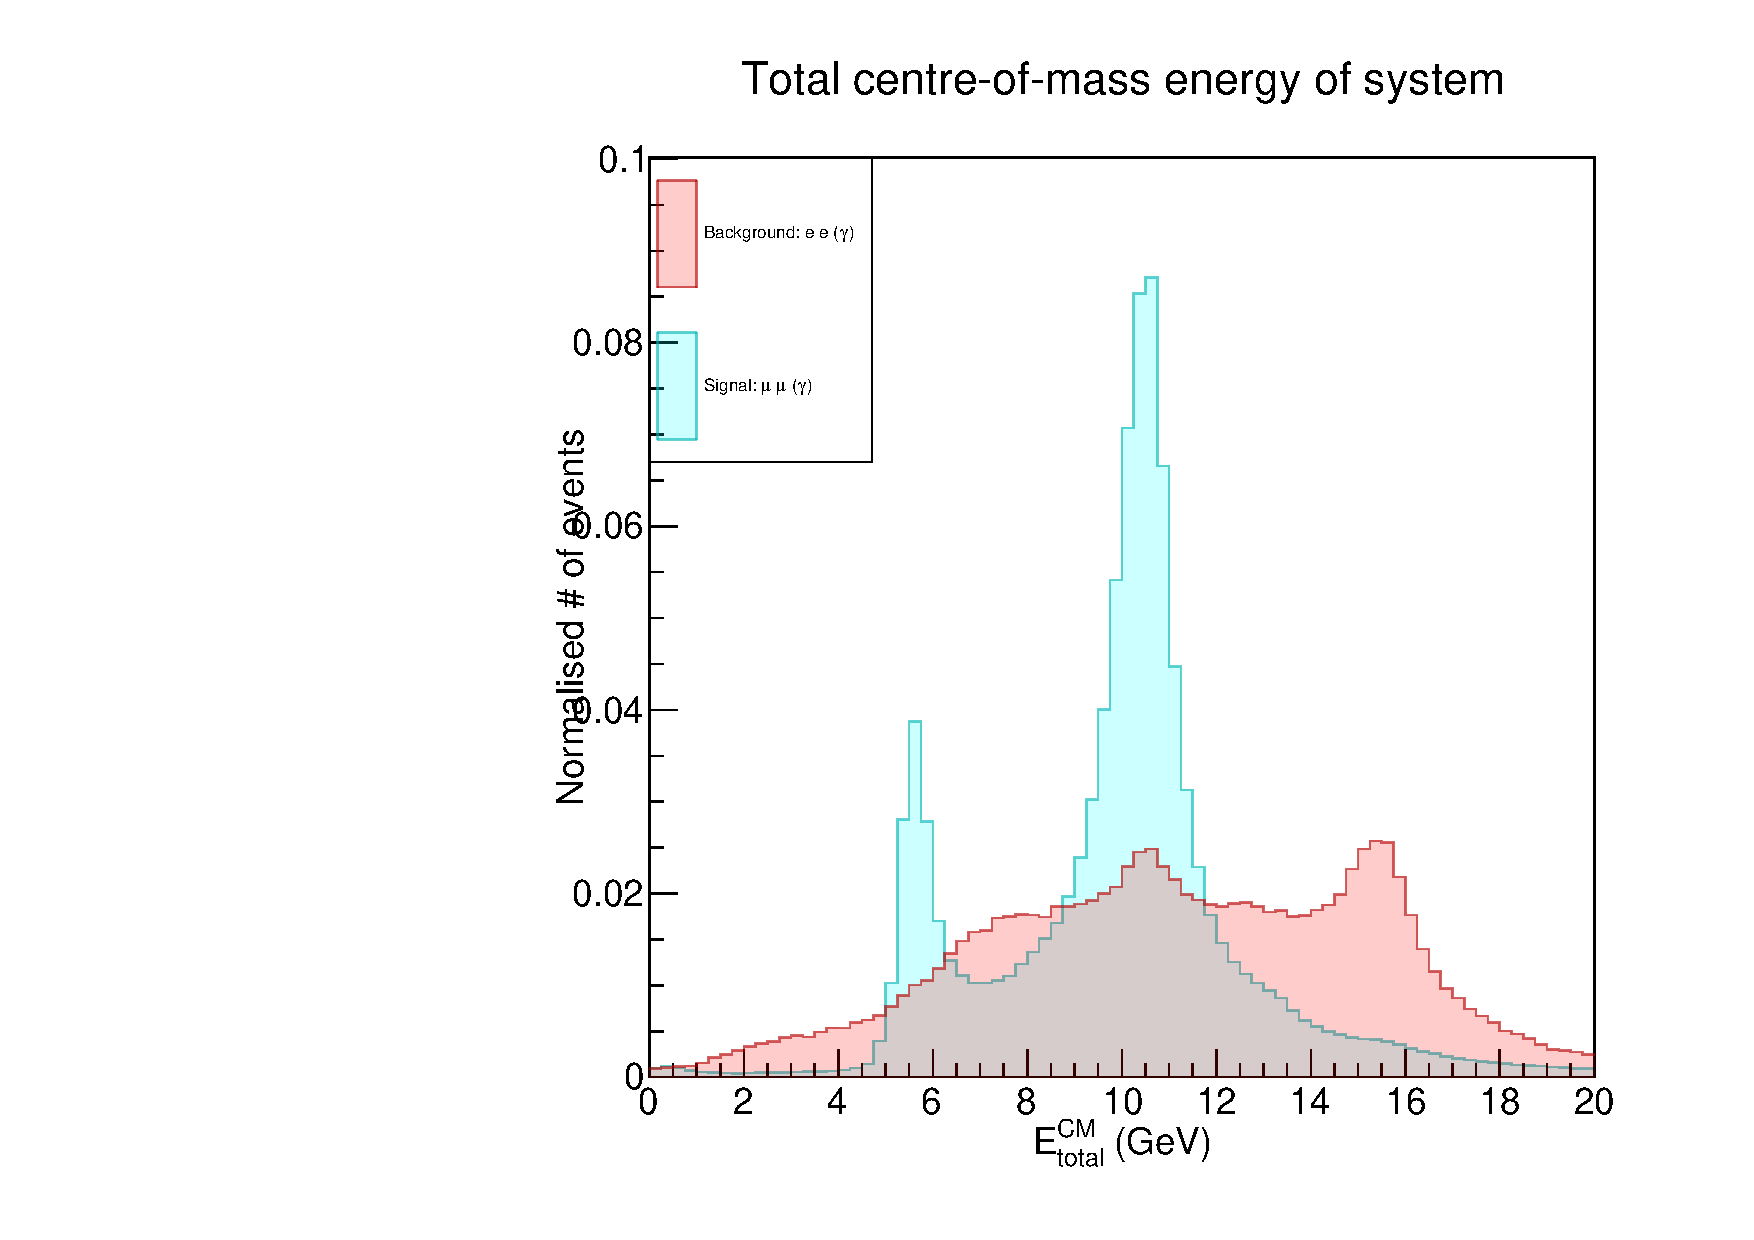
\includegraphics[width=\linewidth]{images/bhabha-mupair-totalCM_E.pdf}
  \captionof{figure}{Bhabha: totalCM E}
  \label{fig:test2}
\end{minipage}
\end{figure}



\pagebreak

%-------------------------------------------------------------------

\chapter{Preselection}

Following reconstruction, preselection criteria were applied to the reconstructed ROOT files. Preselection criteria are defined as distinct from selection criteria in that they remove a minimal amount of signal while removing the more obvious background components; in choosing selection criteria we seek to maximise $S/\sqrt{S+B}$, which may necessarily involve ``cutting out'' some non-neglible amount of signal.

The preselection criteria were selected by inspection of plots of various topology and energy based variables. Different preselection and selection criteria are chosen for each final state mode, due to the different event signatures. A total of 5 variables where chosen for preselection.

\section{Muon mode}

Figures xxx - xxx below show the variables on which preselection criteria were applied, with the specific values for preselection listed in Table xxx. Signal and background efficiencies after preselection are shown in Table XXXX.

98.06\% of reconstructed $\tau\to\mu\gamma$ signal events pass the preselection criteria; around 1,000,000,000 background events out of 2,000,000,000 are removed through this process. Most notably affected by preselecton are the continuum events of which only XXXX\% remain. This reduction is greatly attributed to the clear separation between signal and continuum background in the $E^{\text{CM}}_{\text{total}}$.

\begin{table}[h]
\centering
\begin{tabular}{llllll}
\textbf{symbolic} & \textbf{description} & \cellcolor[HTML]{EFEFEF} \textbf{lower} & \cellcolor[HTML]{EFEFEF} \textbf{upper} & 
\cellcolor[HTML]{C0C0C0} \textbf{lower} & \cellcolor[HTML]{C0C0C0} \textbf{upper}  \\ \hline
$p_{\text{tag}}^{\text{CM}}$  & CM momentum of tag track & --- & $\SI{5.2}{GeV}$ \\
$\cos\theta_{\text{signal}}$ & Cosine of polar angle of signal track & $-0.9$ & --- \\
$E_{\text{total}}^{\text{CM}}$ & Center-of-mass energy of total system  & --- & $\SI{15}{GeV}$ \\
$\lvert\text{thrust}\rvert$ & Magnitude of signal thrust vector* & 0.92 & --- \\
$E_{\text{sum}}^{\text{CM}}$ & Center-of-mass energy of photons and tracks & $\SI{4.5}{GeV}$ & ---
\end{tabular}
\caption{Preselection cuts (muon mode)}
\label{my-label}
\end{table}



    \begin{figure}
        \centering
        \begin{subfigure}[b]{0.475\textwidth}
            \centering
            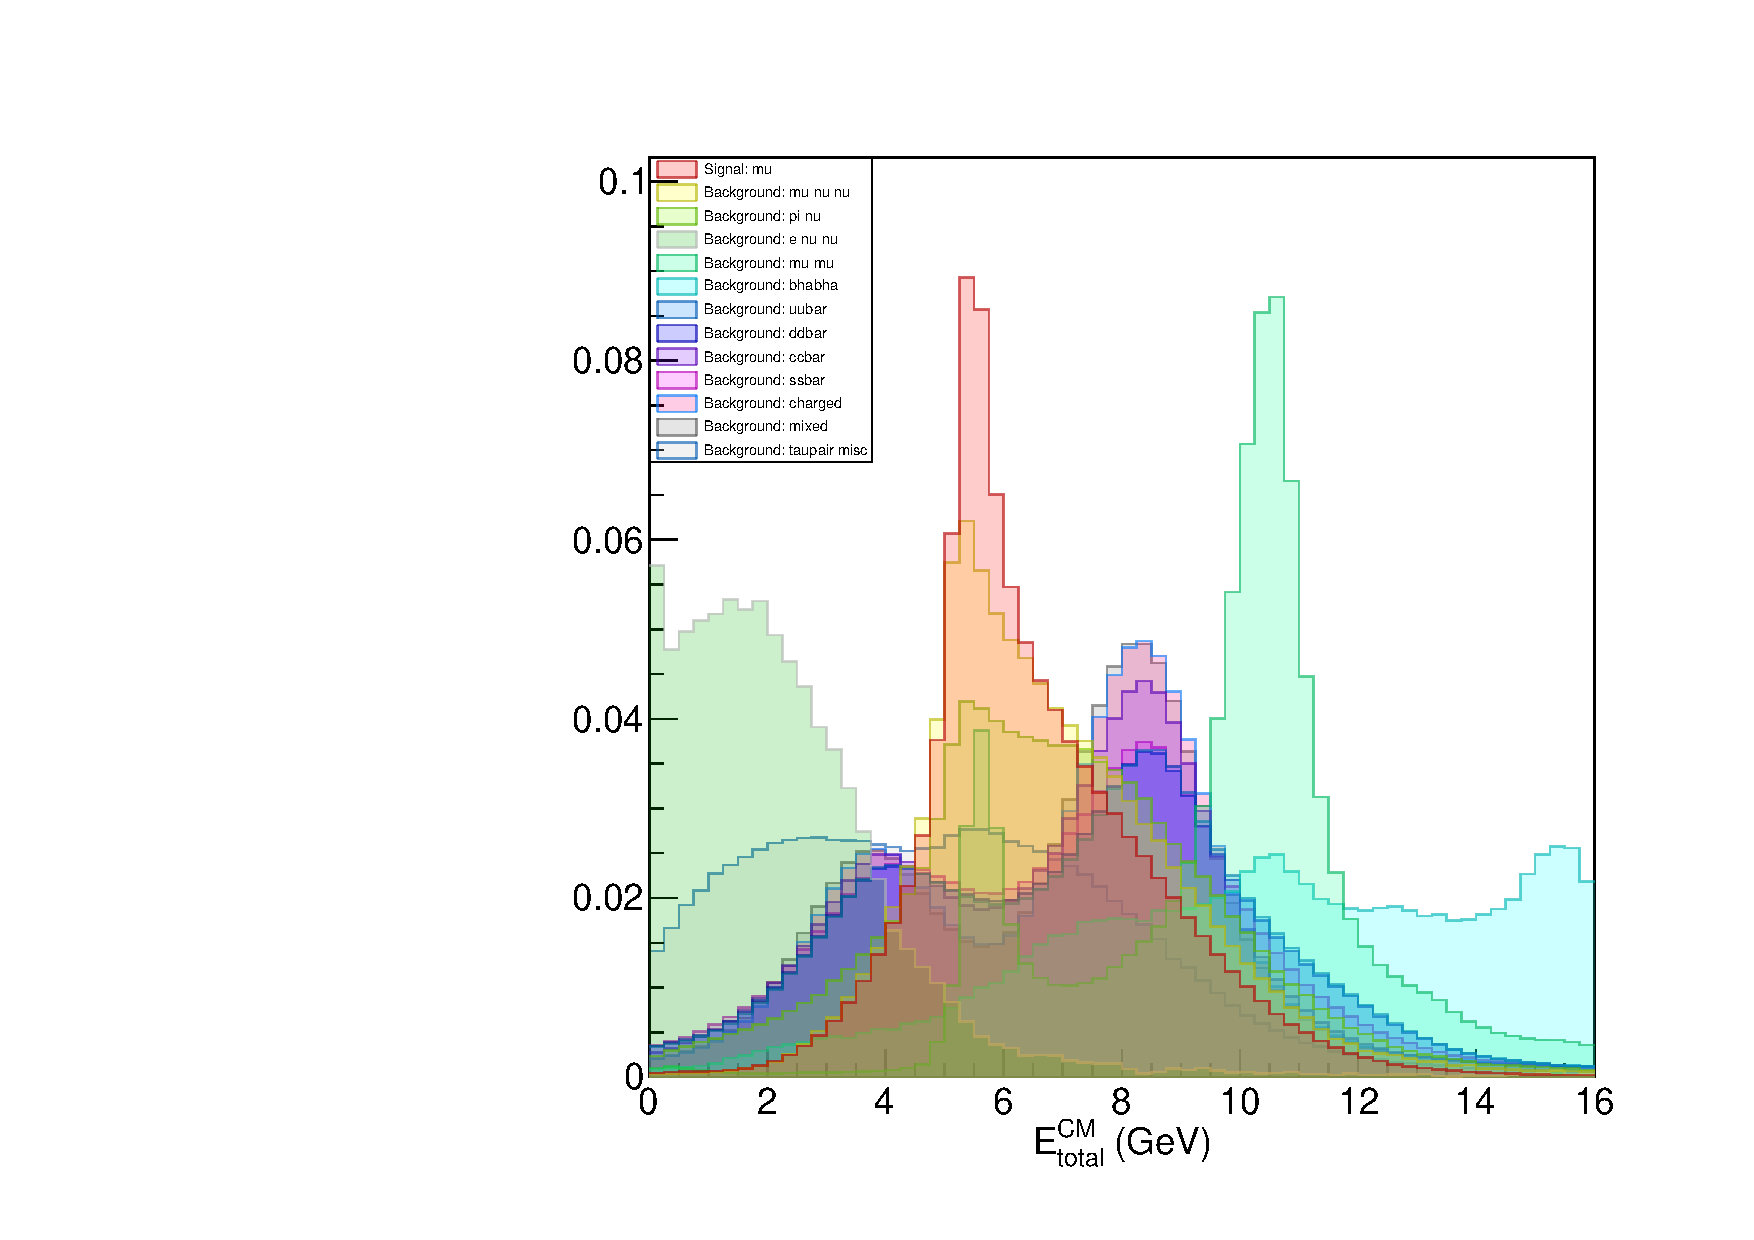
\includegraphics[width=\textwidth]{images/test.pdf}
            \caption[Network2]%
            {{\small Network 1}}    
            \label{fig:mean and std of net14}
        \end{subfigure}
        \hfill
        \begin{subfigure}[b]{0.475\textwidth}  
            \centering 
            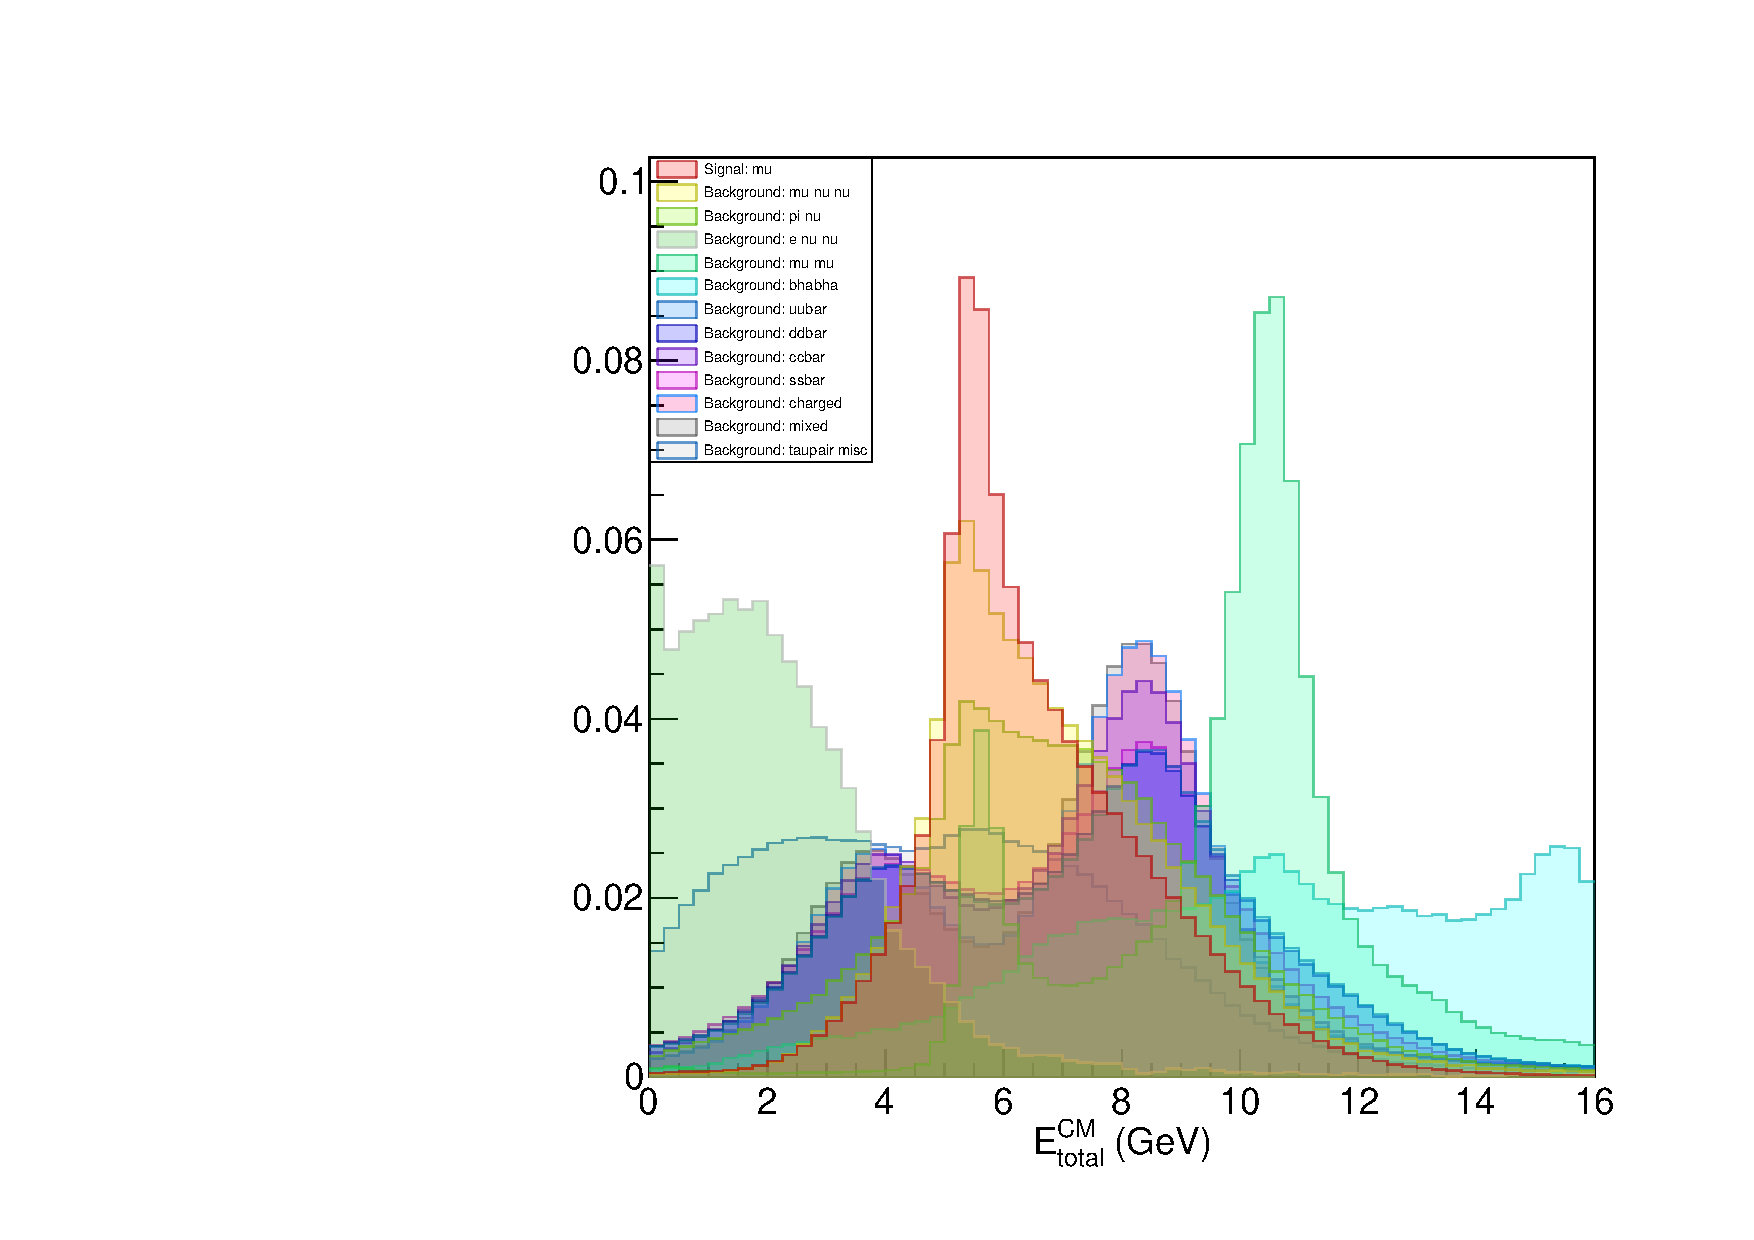
\includegraphics[width=\textwidth]{images/test.pdf}
            \caption[]%
            {{\small Network 2}}    
            \label{fig:mean and std of net24}
        \end{subfigure}
        \vskip\baselineskip
        \begin{subfigure}[b]{0.475\textwidth}   
            \centering 
            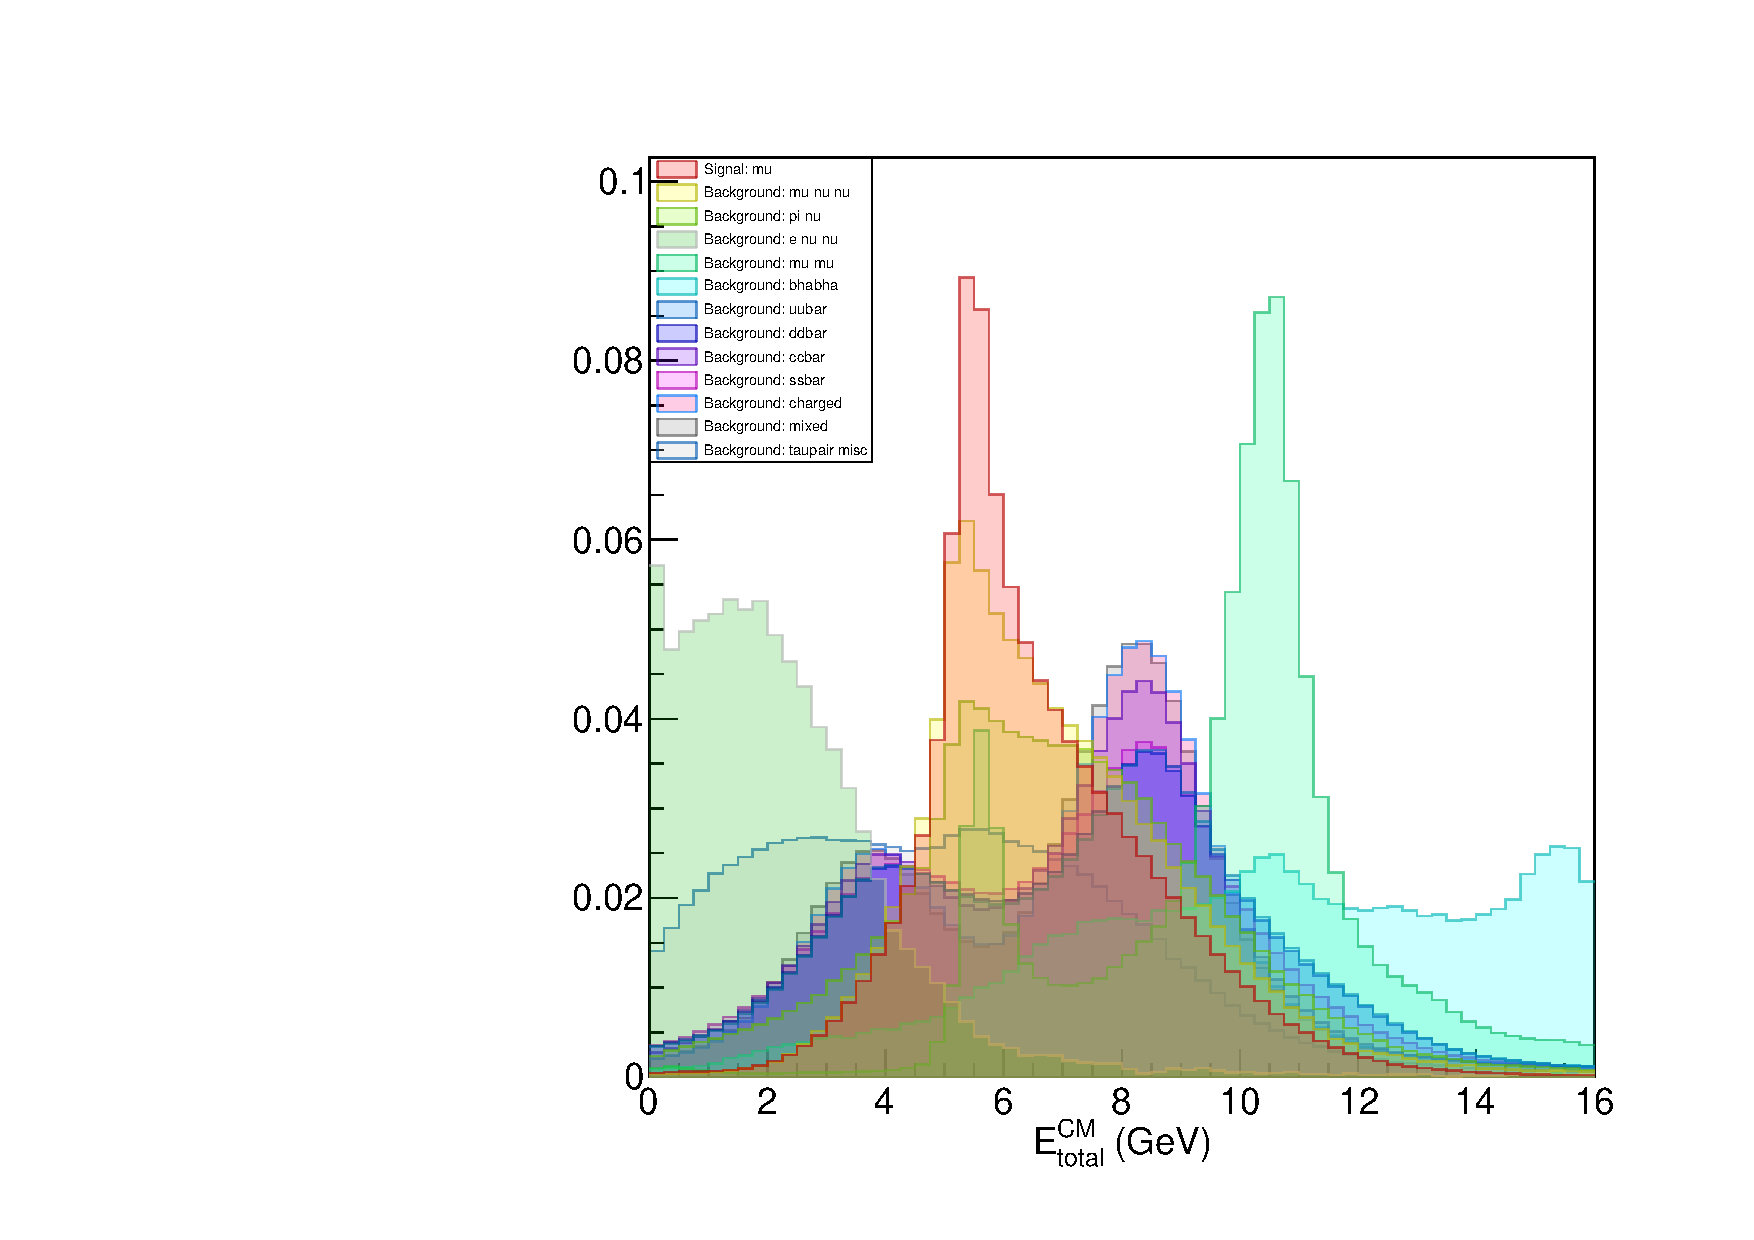
\includegraphics[width=\textwidth]{images/test.pdf}
            \caption[]%
            {{\small Network 3}}    
            \label{fig:mean and std of net34}
        \end{subfigure}
        \quad
        \begin{subfigure}[b]{0.475\textwidth}   
            \centering 
            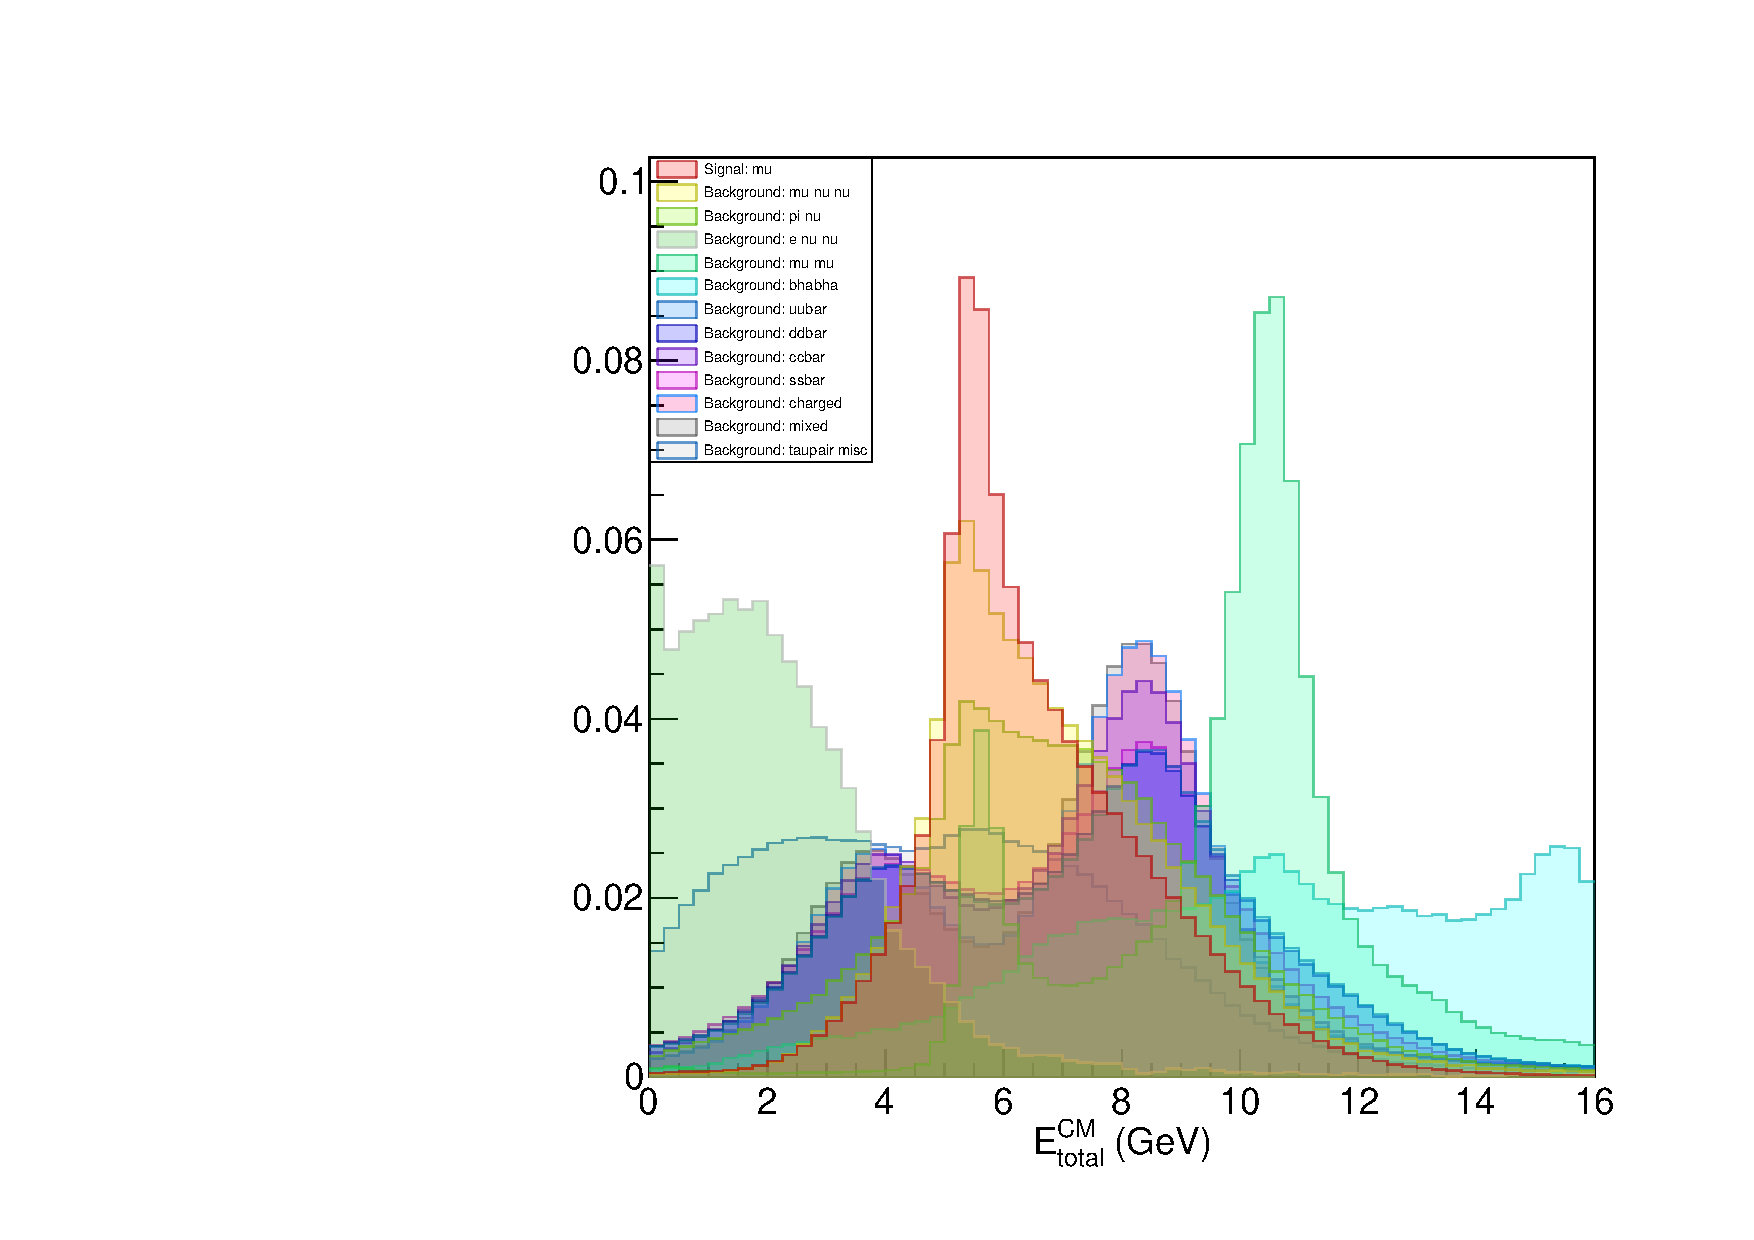
\includegraphics[width=\textwidth]{images/test.pdf}
            \caption[]%
            {{\small Network 4}}    
            \label{fig:mean and std of net44}
        \end{subfigure}
        \label{fig:mean and std of nets}
                \vskip\baselineskip
                \begin{subfigure}[b]{0.475\textwidth}   
            \centering 
            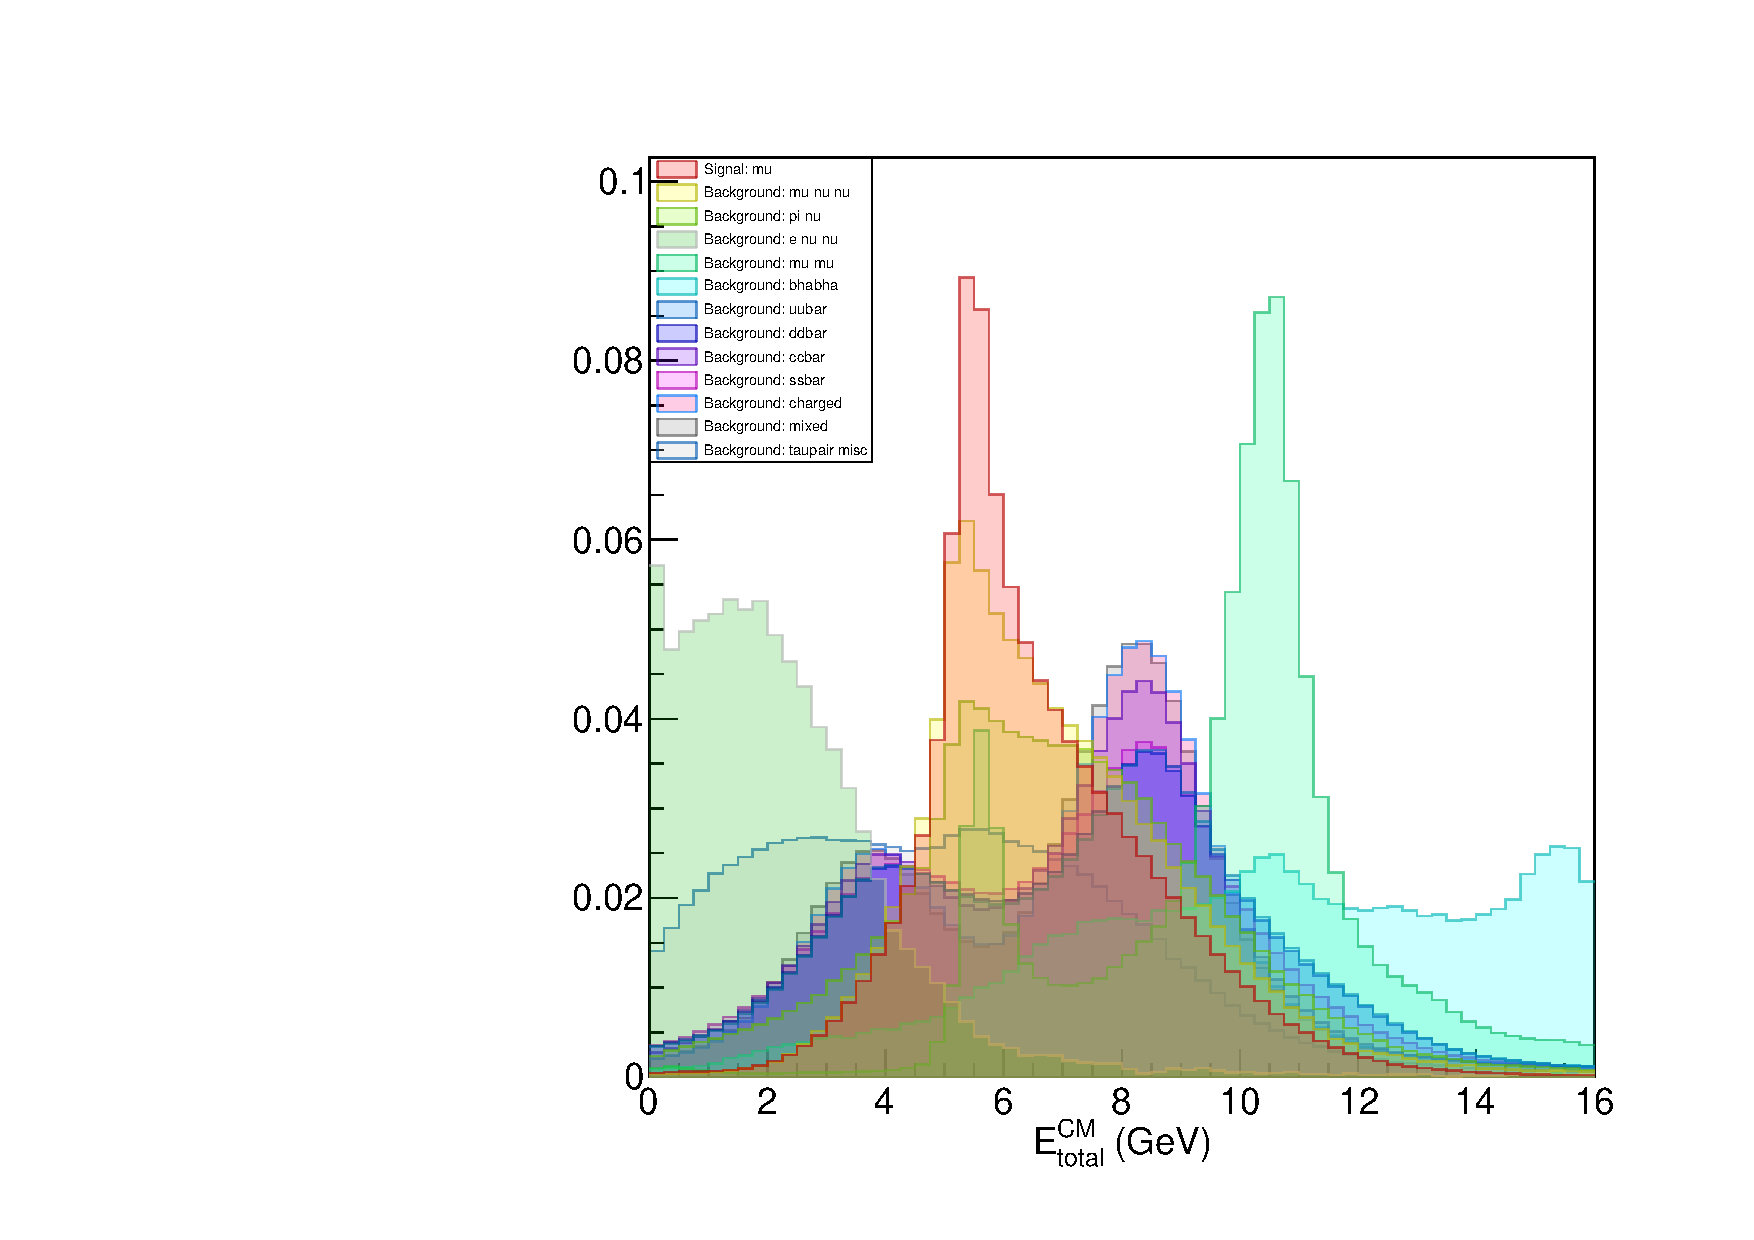
\includegraphics[width=\textwidth]{images/test.pdf}
            \caption[]%
            {{\small Network 3}}    
            \label{fig:mean and std of net34}
        \end{subfigure}
                \caption[ The average and standard deviation of critical parameters ]
        {\small The average and standard deviation of critical parameters: Region R4} 
    \end{figure}


\begin{table}[h]
\centering
\begin{tabular}{llll}
\textbf{MCtype} & \textbf{events in (reconstructed)} & \textbf{events out (preselection)} & $\mathbf{\epsilon_{\text{ps}}}$\\ \hline
\rowcolor[HTML]{EFEFEF}
$\tau\to\mu\gamma$ & 2914095 & 2857577 & 98.06\%	\\
$\tau\to\mu\nu\nu$ & \num{32d6} & 153730 & 0.48\%\\
$\tau\to\pi\nu$ & \num{38d6} & 102813 & 0.27\%\\
$\tau\to e\nu\nu$ & \num{4.8d6} & 13322 & 0.28\%\\
$\tau\to\text{generic}$ & \num{63d6} & 47274 & 0.08\%\\
$e^+ e^-\to\mu^+\mu^-(\gamma)$ & \num{16.9332d6} & 8099760 & 47.83\%	\\
$e^+ e^-\to e^+e^-\gamma$ & \num{1.403d6} & 185377 & 13.21\%	\\
$e^+ e^-\to u\bar{u}$ & 20794 & 7352 & 35.36\%	\\
$e^+ e^-\to d\bar{d}$ & 20199 & 7259 & 35.94\%	\\
$e^+ e^-\to c\bar{c}$ & 13688 & 2424 & 17.71\%	\\
$e^+ e^-\to s\bar{s}$ & 15979 & 4856 & 30.39\%	\\
$e^+ e^-\to B^+B^-$ & 24907 & 3636 & 14.60\%	\\
$e^+ e^-\to B^0 \bar{B}^0$ & 26058 & 3550 & 13.62\%
\end{tabular}
\caption{Preselection efficiency (muon mode)}
\label{my-label}
\end{table}

\section{Electron mode}

Separate preselection criteria was chosen for the electron mode. 


\begin{figure}[h]
\centering
\begin{minipage}{.5\textwidth}
  \centering
  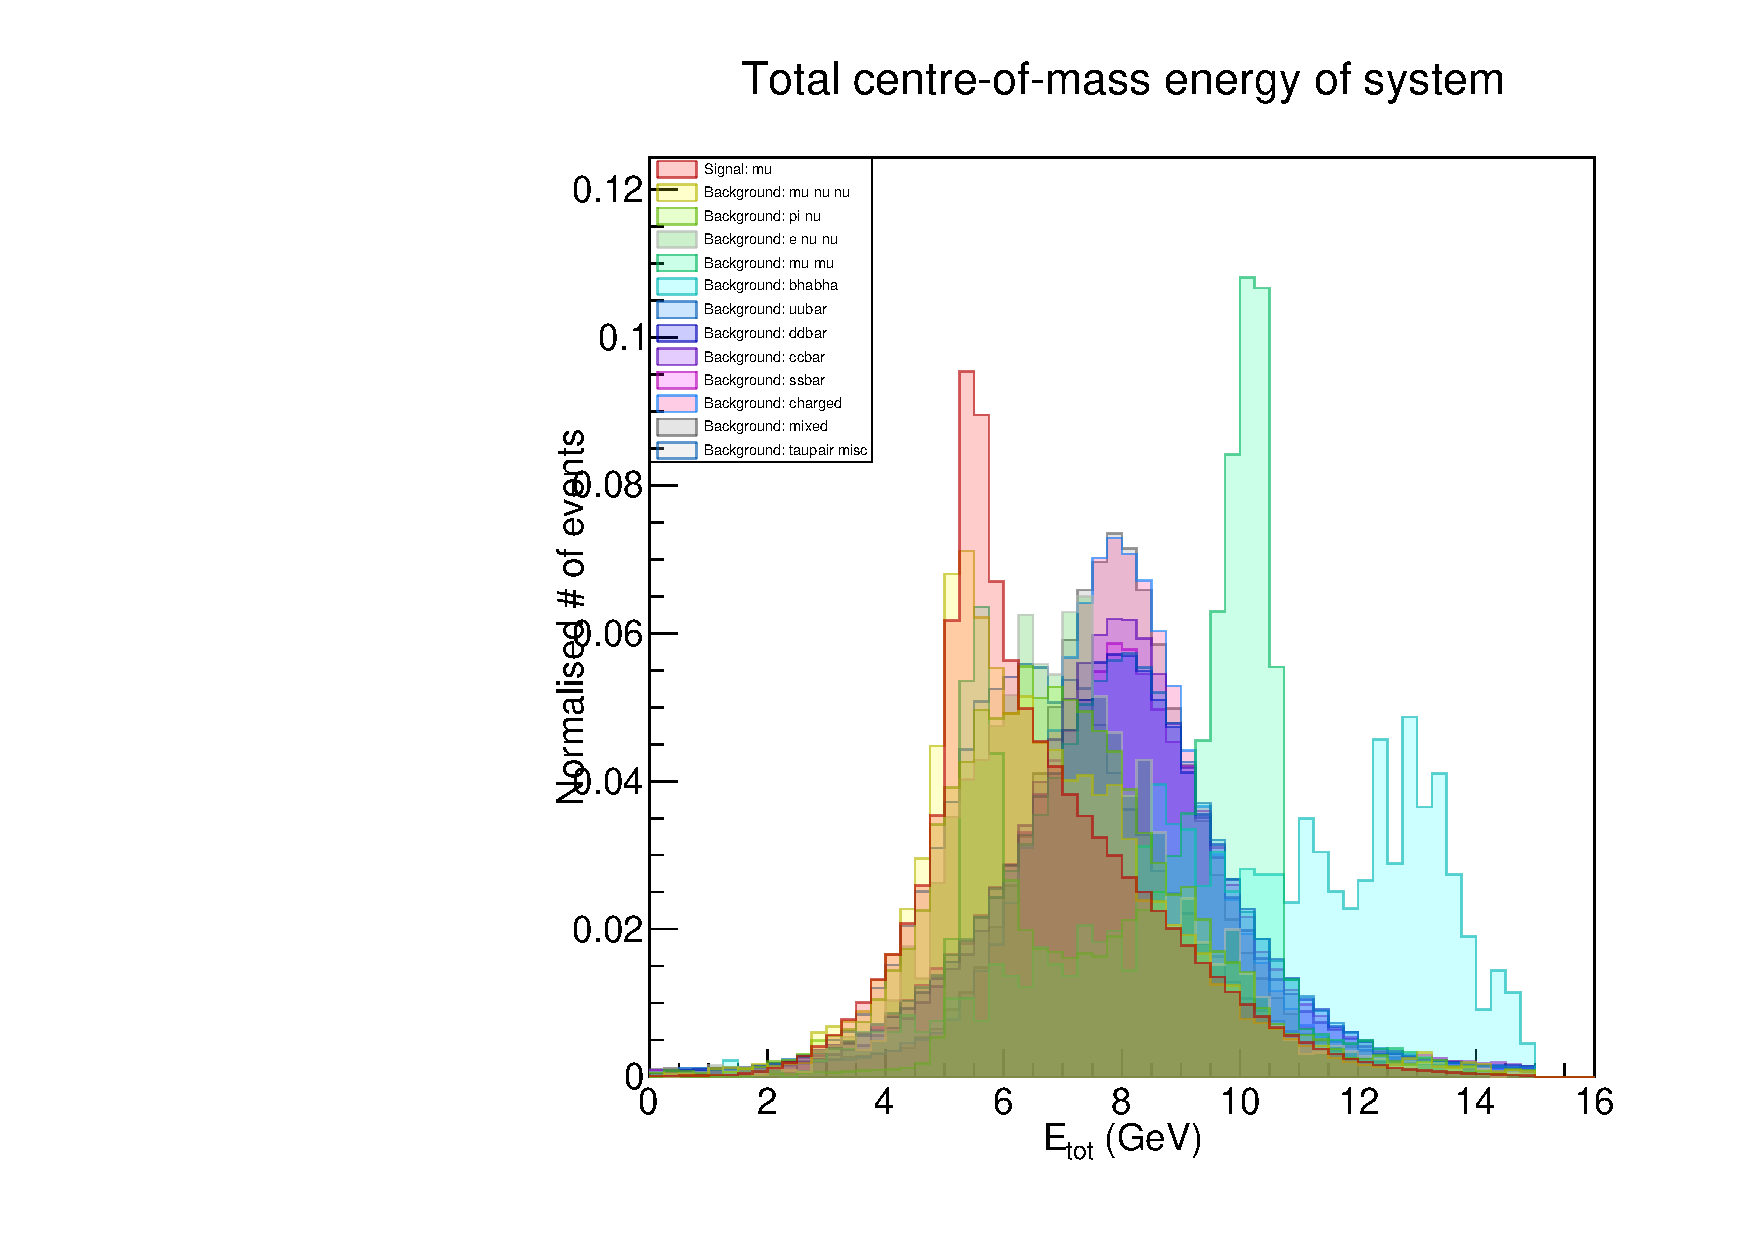
\includegraphics[width=\linewidth]{images/stack/stack_cut6_totalCM_E.pdf}
  \captionof{figure}{A figure}
  \label{fig:test1}
\end{minipage}%
\begin{minipage}{.5\textwidth}
  \centering
  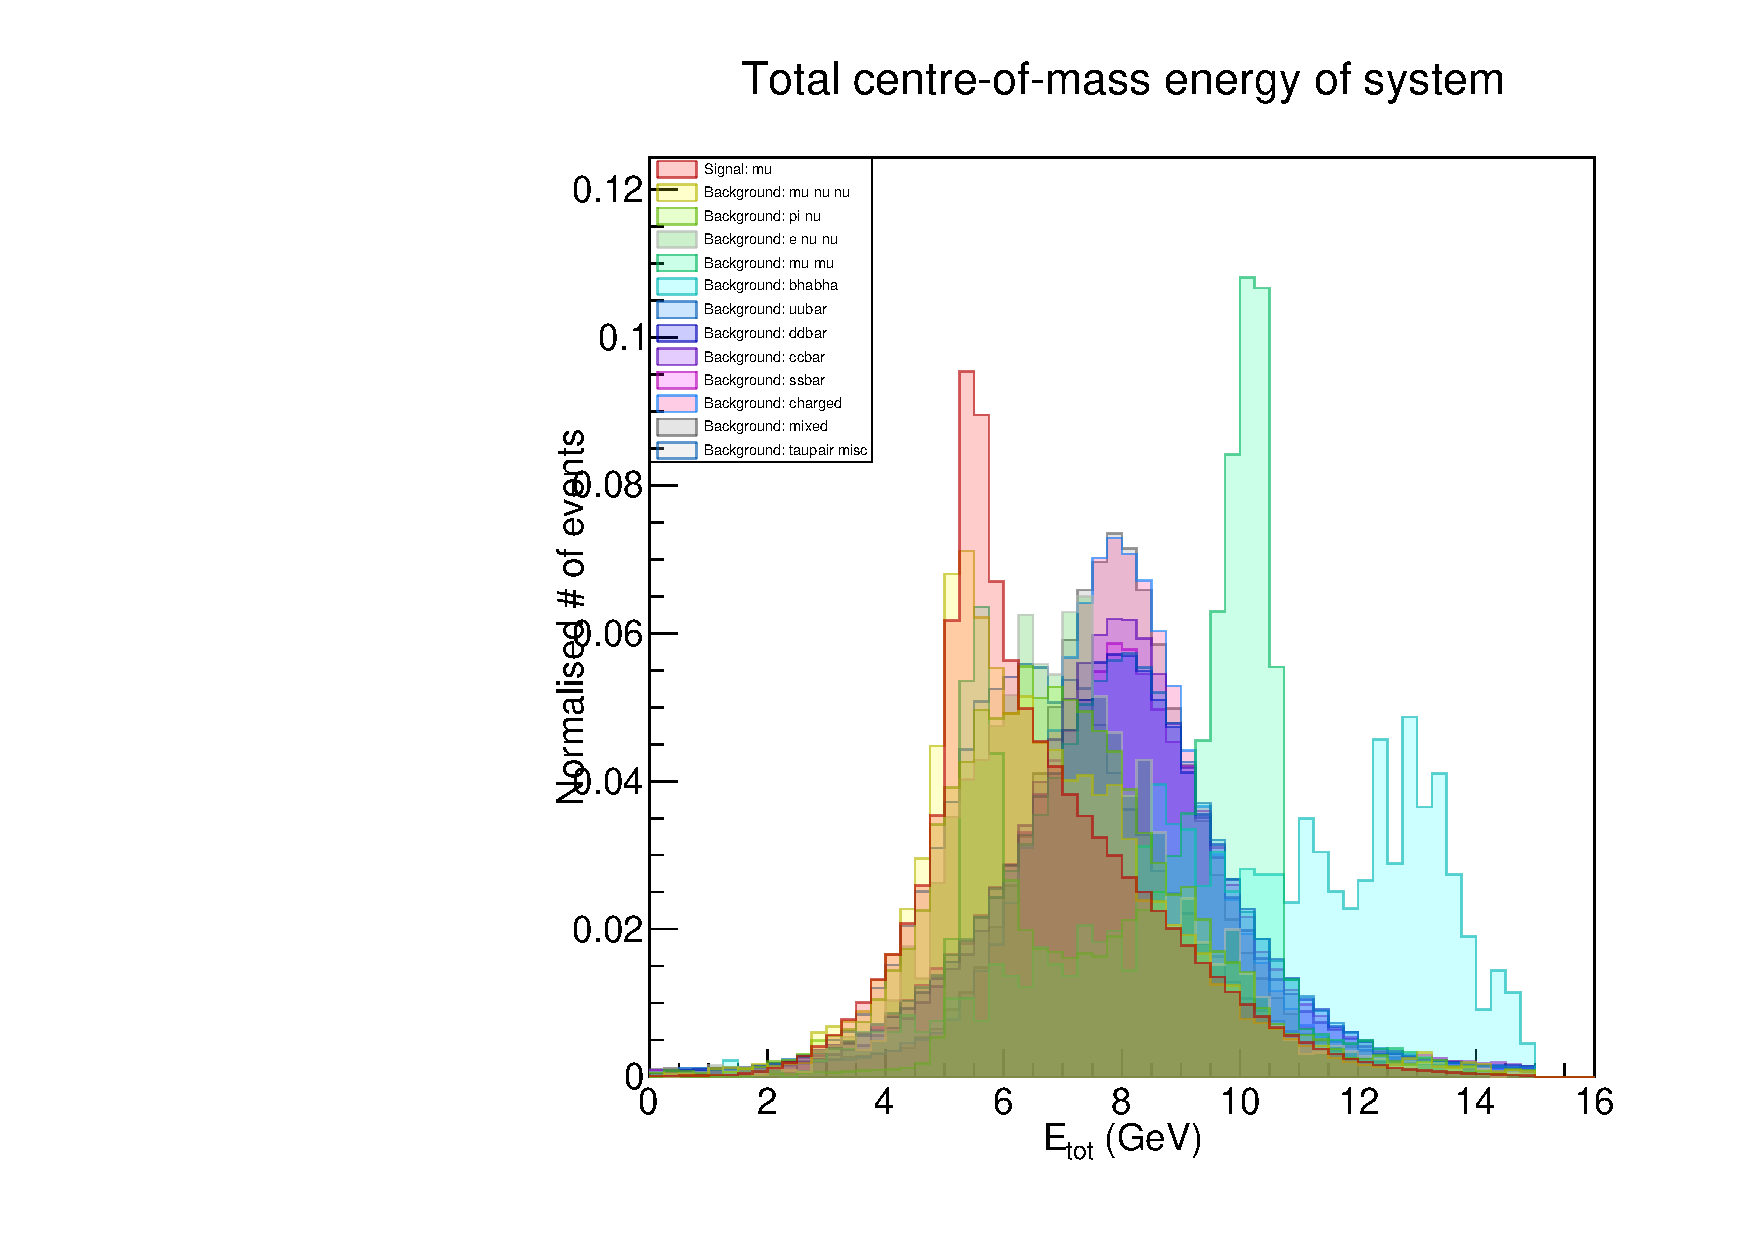
\includegraphics[width=\linewidth]{images/stack/stack_cut6_totalCM_E.pdf}
  \captionof{figure}{Another figure}
  \label{fig:test2}
\end{minipage}
\end{figure}

\begin{table}[h]
\centering
\begin{tabular}{llll}
\textbf{symbolic} & \textbf{description} & \textbf{lower} & \textbf{upper} \\ \hline
$p_{\text{tag}}^{\text{CM}}$  & CM momentum of tag track & --- & $\SI{5}{GeV}$ \\
$\cos\theta_{\text{signal}}$ & Cosine of polar angle of signal track & $-0.975$ & --- \\
$E_{\text{total}}^{\text{CM}}$ & Center-of-mass energy of total system  & --- & $\SI{15}{GeV}$ \\
$\lvert\text{thrust}\rvert$ & Magnitude of signal thrust vector* & 0.92 & --- \\
$E_{\text{sum}}^{\text{CM}}$ & Center-of-mass energy of photons and tracks & $\SI{4.5}{GeV}$ & ---
\end{tabular}
\caption{Preselection cuts (electron mode)}
\label{my-label}
\end{table}

  \begin{figure}
        \centering
        \begin{subfigure}[b]{0.475\textwidth}
            \centering
            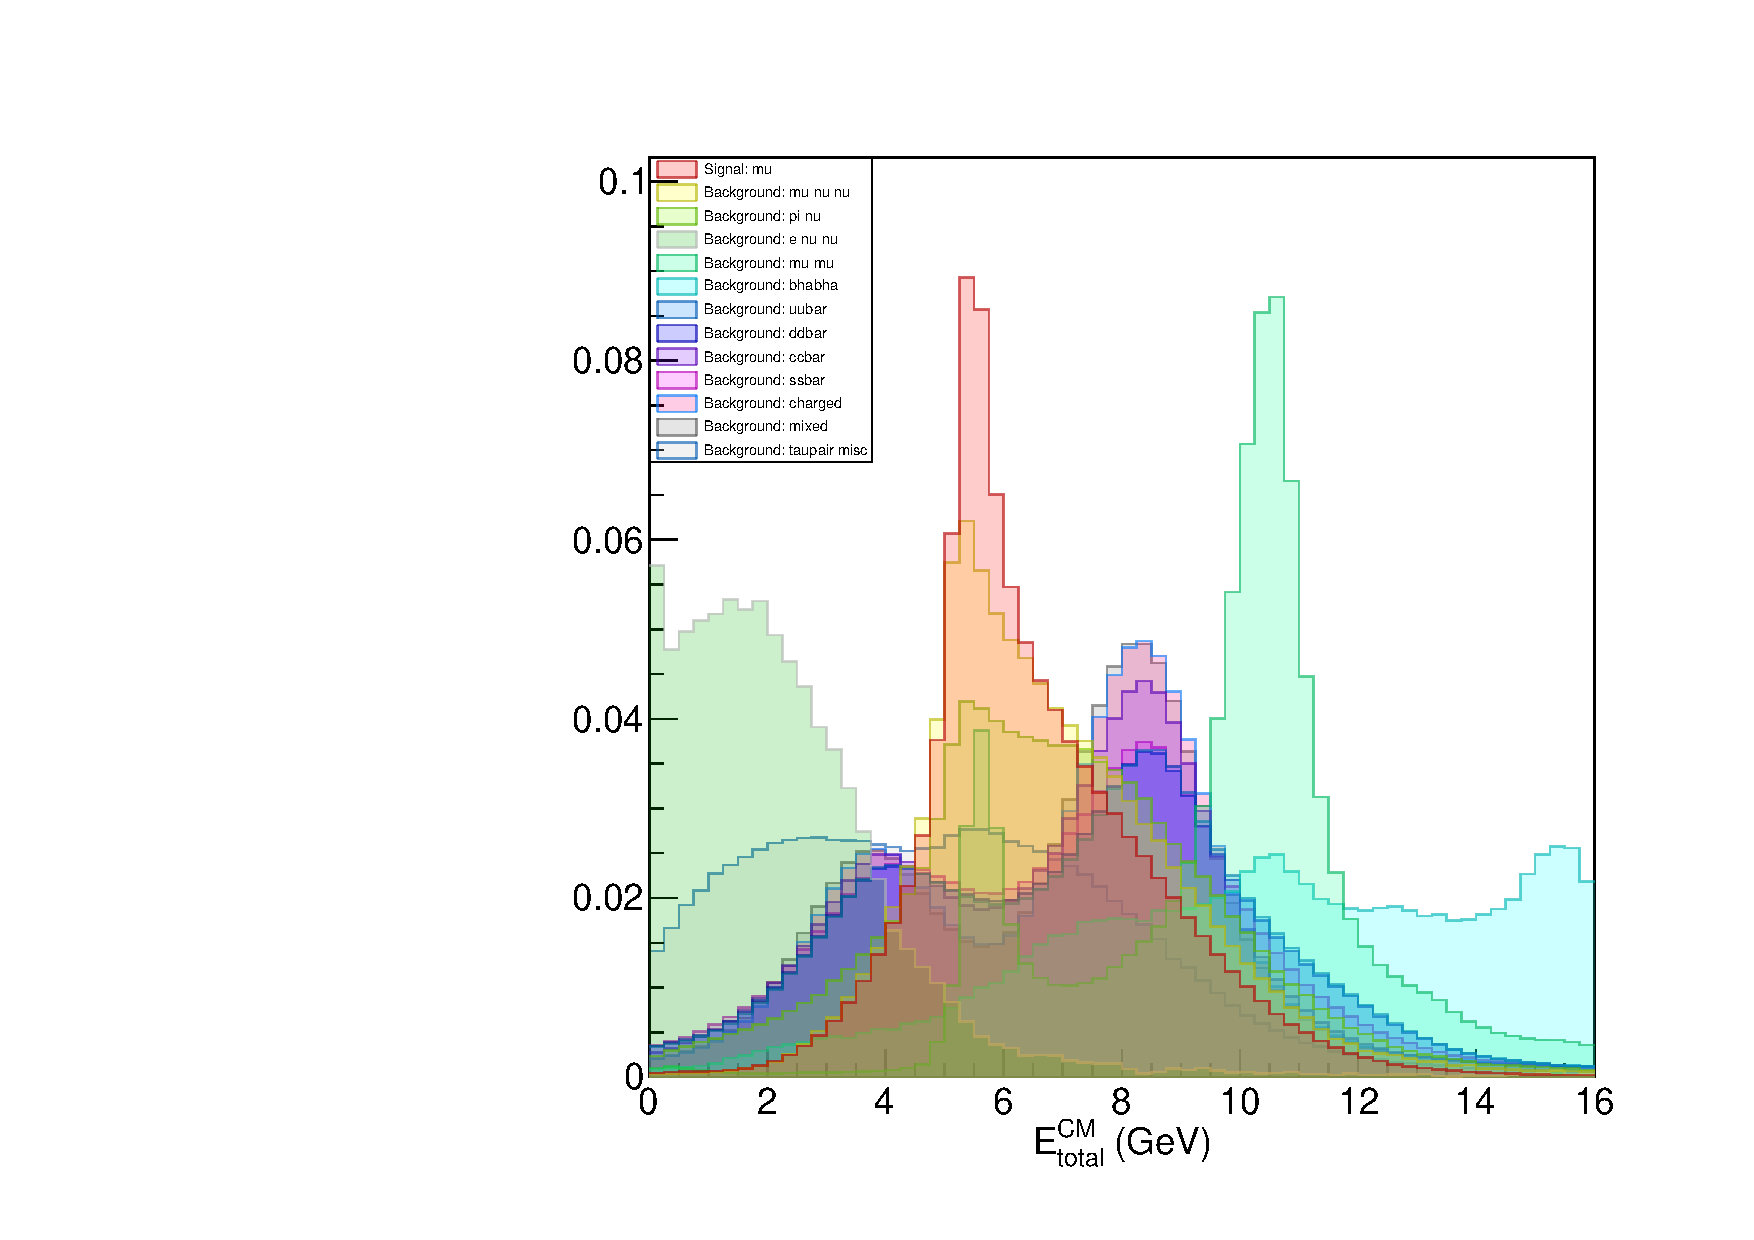
\includegraphics[width=\textwidth]{images/test.pdf}
            \caption[Network2]%
            {{\small Network 1}}    
            \label{fig:mean and std of net14}
        \end{subfigure}
        \hfill
        \begin{subfigure}[b]{0.475\textwidth}  
            \centering 
            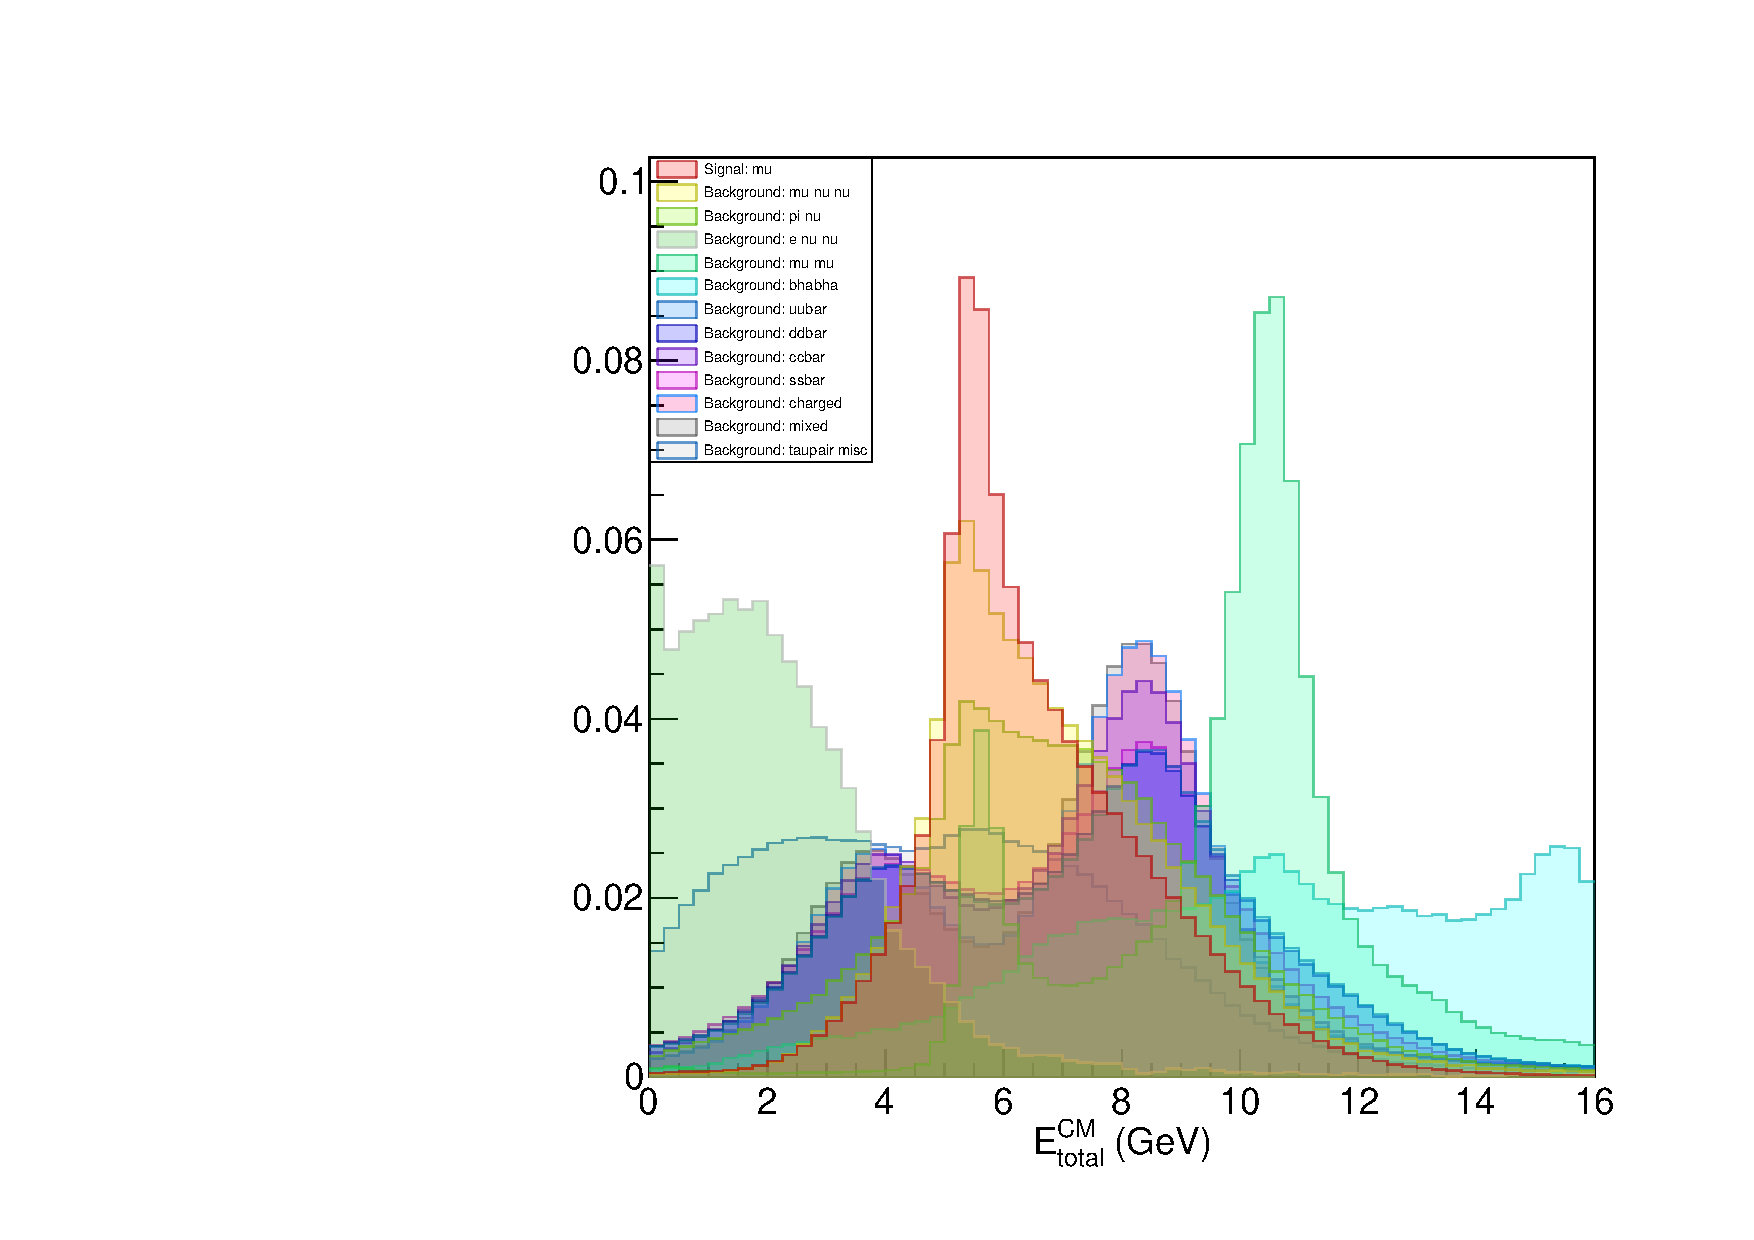
\includegraphics[width=\textwidth]{images/test.pdf}
            \caption[]%
            {{\small Network 2}}    
            \label{fig:mean and std of net24}
        \end{subfigure}
        \vskip\baselineskip
        \begin{subfigure}[b]{0.475\textwidth}   
            \centering 
            \includegraphics[width=\textwidth]{images/test.pdf}
            \caption[]%
            {{\small Network 3}}    
            \label{fig:mean and std of net34}
        \end{subfigure}
        \quad
        \begin{subfigure}[b]{0.475\textwidth}   
            \centering 
            \includegraphics[width=\textwidth]{images/test.pdf}
            \caption[]%
            {{\small Network 4}}    
            \label{fig:mean and std of net44}
        \end{subfigure}
        \label{fig:mean and std of nets}
                \vskip\baselineskip
                \begin{subfigure}[b]{0.475\textwidth}   
            \centering 
            \includegraphics[width=\textwidth]{images/test.pdf}
            \caption[]%
            {{\small Network 3}}    
            \label{fig:mean and std of net34}
        \end{subfigure}
                \caption[ The average and standard deviation of critical parameters ]
        {\small The average and standard deviation of critical parameters: Region R4} 
        \end{figure}


\begin{table}[h]
\centering
\begin{tabular}{llll}
\textbf{MCtype} & \textbf{events in (reconstructed)} & \textbf{events out (preselection)} & $\mathbf{\epsilon_{\text{ps}}}$\\ \hline
\rowcolor[HTML]{EFEFEF}
$\tau\to\mu\gamma$ & 2914095 & 2857577 & 98.06\%	\\
$\tau\to\mu\nu\nu$ & \num{32d6} & 153730 & 0.48\%\\
$\tau\to\pi\nu$ & \num{38d6} & 102813 & 0.27\%\\
$\tau\to e\nu\nu$ & \num{4.8d6} & 13322 & 0.28\%\\
$\tau\to\text{generic}$ & \num{63d6} & 47274 & 0.08\%\\
$e^+ e^-\to\mu^+\mu^-(\gamma)$ & \num{16.9332d6} & 8099760 & 47.83\%	\\
$e^+ e^-\to e^+e^-\gamma$ & \num{1.403d6} & 185377 & 13.21\%	\\
$e^+ e^-\to u\bar{u}$ & 20794 & 7352 & 35.36\%	\\
$e^+ e^-\to d\bar{d}$ & 20199 & 7259 & 35.94\%	\\
$e^+ e^-\to c\bar{c}$ & 13688 & 2424 & 17.71\%	\\
$e^+ e^-\to s\bar{s}$ & 15979 & 4856 & 30.39\%	\\
$e^+ e^-\to B^+B^-$ & 24907 & 3636 & 14.60\%	\\
$e^+ e^-\to B^0 \bar{B}^0$ & 26058 & 3550 & 13.62\%
\end{tabular}
\caption{Preselection efficiency (muon mode)}
\label{my-label}
\end{table}

\pagebreak

%-------------------------------------------------------------------

\chapter{Correlation}

The final signal region in which events will be selected from lies in $\Delta E$ vs. $M_{\text{inv}}$ space. To avoid biasing event selection, only loose cuts are applied to these variables throughout. We also investigate the correlation between these signal variables and other variables which we may cut over, to avoid introducing bias through these correlations. 

???

\pagebreak

%-------------------------------------------------------------------

\chapter{Signal optimisation}

A total of XXXX selection cuts were performed.

In optimizing the selection cuts, two distinct methods were used. In the first method, selection cuts were manually chosen based on a combination of individual threshold efficiencies and visual inspection. For individual threshold efficiencies, each cut was performed over all MC types with no other cuts, and the cut ``threshold'' varied each time. The output files were then used to produce figure-of-merit plots, where $S/\sqrt{S+B}$ was plotted against threshold; see below for a few examples. Cuts were applied in ``groups'', with more immediately clear cuts being performed first to reduce background for later cuts. After all cuts were performed, the signal and background efficiencies were as below, with the expected number of events.

EFFICIENCIES

The second method used multivariate analysis (MVA) methods, available through the Toolkit for Multivariate Analysis (TMVA). ??? haven't actually done this yet.

\pagebreak

\begin{table}[h]
\centering
\begin{tabular}{lllll}
\textbf{cut number} & \textbf{symbolic} & \textbf{description} & \textbf{lower} & \textbf{upper} \\ \hline
\textbf{muCM\_P} & $p_{\text{signal}}^{\text{CM}}$  & CM momentum of signal track  &  &  \\
\textbf{tagtrackCM\_P} & $p_{\text{tag}}^{\text{CM}}$  & CM momentum of tag track &  &  \\
\textbf{mu\_Pt} & $p_{t~\text{signal}}$ & Transverse momentum of signal track &  &  \\
\textbf{mu\_Pt} & $p_{t~\text{tag}}$ & Transverse momentum of tag track &  &  \\
\textbf{muCosTheta} & $\cos\theta_{\text{signal}}$ & Cosine of polar angle of signal track &  &  \\
\textbf{tagtrackCosTheta} & $\cos\theta_{\text{tag}}$ & Cosine of polar angle of tag track &  &  \\
\textbf{totalCM\_E} & $E_{\text{total}}^{\text{CM}}$ & Center-of-mass energy of total system  &  &  \\
\textbf{thrustSignal} & $\lvert\text{thrust}_{\text{signal}}\rvert$ & Magnitude of signal thrust vector* &  &  \\
\textbf{signalPIDmu} & $\mu\text{-ID}_{\text{signal}}$ & $\mu$ PID of signal track &  &  \\
\textbf{mu\_P} & $p_{\text{signal}}$  & Momentum of signal track &  &  \\
\textbf{tagPIDmu} & $\mu\text{-ID}_{\text{tag}}$ & $\mu$ PID of tag track &  &  \\
\textbf{gamma\_E} & $E_{\gamma}$ & Energy of signal photon &  &  \\
 & $\cos\theta_{\gamma}$ & Cosine of polar angle of signal photon &  &  \\
 & $\cos\theta^{\text{CM}}_{\text{signal}-\gamma}$ & Cosine of angle between signal track and signal photon in CM &  &  \\
\textbf{sumCM\_E} & $E_{\text{sum}}^{\text{CM}}$ & Center-of-mass energy of photons and tracks &  &  \\
\textbf{tracksCMOpeningTheta} &  & Opening angle between signal and tag track &  &  \\
\textbf{helicityCosTheta} &  & Cosine of the helicity angle &  &  \\
 & $\cos\theta^{\text{CM}}_{\text{miss-tag}}$ & Opening angle between tag track and missing momentum &  &  \\
\textbf{tracks} & $n_{\text{tracks}}$ & Number of charged tracks &  &  \\
\textbf{signalPIDk} & $\text{K-ID}_{\text{signal}}$ & K PID of signal track &  &  \\
\textbf{signalPIDpi} & $\pi\text{-ID}_{\text{signal}}$ & $\pi$ PID of signal track &  &  \\
\textbf{signalPIDe} & $\text{e-ID}_{\text{signal}}$ & e PID of signal track &  &  \\
\textbf{clusterNHits} &  & timing of this cluster &  &  \\
\textbf{clusterUncorrE} &  & uncorrected cluster energy &  &  \\
\textbf{clusterHighE} &  & highest crystal energy in the cluster &  &  \\
\textbf{clusterTiming} &  & timing of this cluster &  &  \\
\textbf{signalTrPval} &  & Signal track fit pvalue &  &  \\
\textbf{tagTrPval} &  & Tag track fit pvalue &  &  \\
\textbf{cosTBz} &  & Cosine of the angle between the thrust axis of the signal track and the z-axis &  &  \\
\textbf{cc1} &  & Cleo cone 1 &  &  \\
\textbf{hso00} &  & Hso(0,0) &  &  \\
\textbf{neutralECLEnergy} &  & Total energy of all neutral ECLClusters &  & 
\end{tabular}
\caption{Selection criteria}
\label{my-label}
\end{table}


\pagebreak

\emph{Note that these cluster based quantities apply to particles constructed from ECL clusters} (from NtupleTool page).


\pagebreak

%-------------------------------------------------------------------

\chapter{Signal region and event selection}

After selection, we are left with a far reduced number of background events and a non-neglible amount of expected signal events. We can now analyse events within the signal region. This is a region in $\Delta E$ vs $M_{\text{inv}}$ space, with $-0.2 < \Delta E < 0.2$, and $1.7 < M_{\text{inv}} < 1.8$.

$\Delta E$ is the energy difference between the reconstructed particles and beam energy, calculated as ????. $M_{\text{inv}}$ is the invariant mass of the reconstructed signal tau; experimentally the tau has a mass of $\SI{1.7}{GeV/c}$. These variables have only been cut on very loosely up until this point to avoid bias.

\pagebreak

%-------------------------------------------------------------------

\chapter{Conclusion}

We analysed an $\SI{1000}{fb^-1}$ sample of Belle II MC comprising a range of common backgrounds, reconstructed and simulated using Super-KEKB geometries. We were able to provide estimates on possible improves to $\tau\to\ell\gamma$ branching fractions;

\begin{align}
\mathcal{Br}(\tau\to\mu\gamma) &= XXX \pm XXX,\\
\mathcal{Br}(\tau\to e\gamma) &= XXX \pm XXX.
\end{align}

These are consistent with predictions made by the Belle II Collaboration [REF].


\section{Future improvements}

This analysis could be extended to run over actual Belle data. The full dataset of $\SI{1000}{fb^-1}$ is available, and it is possible to this data to be reconstructed in \texttt{basf2}. Previous searches at Belle have used $\SI{200}{fb^-1}$ (???) and $\SI{700}{fb^-1}$; a search over higher luminosity would likely improve the accuracy of some $\tau$ LFV branching fractions.

Could use TMVA (at all? or more? maybe I'll do some). Could use more topological variables such as some of the ones I recently added. Could reconstruct electrons better. Could investigate beam backgrounds and ways to remove it.

\section{Working group status}

WG8 - Tau and low multiplicity.

\section{Expected impact on Belle II}

This research is the first to investigate $\tau$ LFV at Belle II using full analysis of MC. UHHHH



%-----------------------------------------
\newpage
\bibliographystyle{plain}
\bibliography{refs.bib}

\begin{comment}
    \begin{figure*}
        \centering
        \begin{subfigure}[b]{0.475\textwidth}
            \centering
            \includegraphics[width=\textwidth]{images/test.pdf}
            \caption[Network2]%
            {{\small Network 1}}    
            \label{fig:mean and std of net14}
        \end{subfigure}
        \hfill
        \begin{subfigure}[b]{0.475\textwidth}  
            \centering 
            \includegraphics[width=\textwidth]{images/test.pdf}
            \caption[]%
            {{\small Network 2}}    
            \label{fig:mean and std of net24}
        \end{subfigure}
        \vskip\baselineskip
        \begin{subfigure}[b]{0.475\textwidth}   
            \centering 
            \includegraphics[width=\textwidth]{images/test.pdf}
            \caption[]%
            {{\small Network 3}}    
            \label{fig:mean and std of net34}
        \end{subfigure}
        \quad
        \begin{subfigure}[b]{0.475\textwidth}   
            \centering 
            \includegraphics[width=\textwidth]{images/test.pdf}
            \caption[]%
            {{\small Network 4}}    
            \label{fig:mean and std of net44}
        \end{subfigure}
        \caption[ The average and standard deviation of critical parameters ]
        {\small The average and standard deviation of critical parameters: Region R4} 
        \label{fig:mean and std of nets}
    \end{figure*}
    \end{comment}

\end{document}







